% =====================================================================
%  Non-GPU AI Accelerators  --  a lecture on the processors built for
%  deep learning that are not GPUs, 2016--2027: Google's TPUs, the
%  dataflow and wafer-scale designs (Cerebras, SambaNova, Groq,
%  Graphcore, Tenstorrent, Rebellions, Furiosa), the hyperscalers'
%  ASICs (Trainium, Maia, MTIA, the OpenAI-Broadcom part), China's
%  Ascend, Kunlun and Cambricon, the emerging in-memory, photonic and
%  neuromorphic parts, and what the benchmarks and the deals say.
%  Same visual language as "Introduction to GPU Architectures".
%
%  Compile:  pdflatex non_gpu_accelerators_tutorial.tex   (run twice)
%  Self-contained: every figure is TikZ/pgfplots source in this file.
% =====================================================================
\documentclass[aspectratio=169,11pt]{beamer}

% ---------- fonts ----------------------------------------------------
\usepackage[scaled=0.92]{helvet}        % Helvetica-like sans for text
\renewcommand{\ttdefault}{cmtt}         % Computer Modern mono for tokens
\usefonttheme[onlymath]{serif}          % classic serif math
\usepackage{amsmath,amssymb,bm}
\usepackage{booktabs,array}
\usepackage{graphicx}


% ---------- graphics -------------------------------------------------
\usepackage{tikz}
\usepackage{pgfplots}
\pgfplotsset{compat=1.17}
\usetikzlibrary{arrows.meta,positioning,calc,fit,backgrounds,
                decorations.pathreplacing,shapes.geometric}

% ---------- palette --------------------------------------------------
\definecolor{ink}{HTML}{1F2937}     % text, residual stream
\definecolor{muted}{HTML}{6B7280}   % secondary text
\definecolor{hair}{HTML}{D9DDE4}    % hairlines
\definecolor{paper}{HTML}{FCFCFA}   % slide background
\definecolor{tok}{HTML}{5F6F85}     % tokens / tokenizer
\definecolor{emb}{HTML}{0CA678}     % embeddings
\definecolor{posc}{HTML}{7048E8}     % positional information
\definecolor{attn}{HTML}{E8590C}    % attention
\definecolor{mlp}{HTML}{1C7ED6}     % MLP / feed-forward
\definecolor{norm}{HTML}{5C940D}    % normalization
\definecolor{outc}{HTML}{D6336C}     % unembedding / softmax / sampling
\definecolor{trn}{HTML}{9C6644}     % training and scaling
\colorlet{qc}{attn}                 % queries
\definecolor{kc}{HTML}{F59F00}      % keys
\definecolor{vc}{HTML}{1098AD}      % values
\colorlet{kct}{kc!70!black}         % key color, darkened for text
\colorlet{stagec}{ink}              % accent of the current stage

% ---------- beamer look ----------------------------------------------
\setbeamertemplate{navigation symbols}{}
\setbeamercolor{background canvas}{bg=paper}
\setbeamercolor{normal text}{fg=ink}
\setbeamercolor{frametitle}{fg=ink}
\setbeamersize{text margin left=8mm,text margin right=8mm}
\setbeamertemplate{itemize item}{\raisebox{0.25ex}{\tiny\color{stagec}$\blacksquare$}}
\setlength{\leftmargini}{1.1em}
\hyphenpenalty=10000 \exhyphenpenalty=10000   % no hyphenation on slides

% stage = which part of the pipeline the slide belongs to
\newcount\stageno \stageno=1
\newcommand{\stage}[1]{\global\stageno=#1\relax
  \ifcase#1\or\colorlet{stagec}{ink}\or\colorlet{stagec}{tok}%
  \or\colorlet{stagec}{emb}\or\colorlet{stagec}{attn}%
  \or\colorlet{stagec}{mlp}\or\colorlet{stagec}{posc}%
  \or\colorlet{stagec}{trn}\or\colorlet{stagec}{outc}%
  \or\colorlet{stagec}{vc}\or\colorlet{stagec}{ink}\fi}

\makeatletter
% title: accent bar + title + one-line claim (the frame subtitle)
\setbeamertemplate{frametitle}{%
  \nointerlineskip\vspace*{3.6mm}%
  \begin{tikzpicture}[x=1mm,y=1mm]
    \useasboundingbox (0,0) rectangle (144,10.5);
    \fill[stagec,rounded corners=0.5mm] (0,0.3) rectangle (1.5,10.2);
    \ifx\insertframesubtitle\@empty
      \node[anchor=west,inner sep=0,text=ink,
            font=\fontsize{15}{17}\selectfont\bfseries] at (4.2,5.2) {\insertframetitle};
    \else
      \node[anchor=west,inner sep=0,text=ink,
            font=\fontsize{15}{17}\selectfont\bfseries] at (4.2,7.1) {\insertframetitle};
      \node[anchor=west,inner sep=0,text=muted,
            font=\fontsize{8.6}{10}\selectfont] at (4.2,2.0) {\insertframesubtitle};
    \fi
  \end{tikzpicture}}
\makeatother

% footer: pipeline strip with the current stage lit, plus page number
\setbeamertemplate{footline}{%
  
\begin{tikzpicture}[x=1mm,y=1mm]
    \useasboundingbox (0,0) rectangle (160,7.2);
    \coordinate (c0) at (7.2,4.0);
    \foreach \lab/\col [count=\i,remember=\i as \prev (initially 0)] in
      {Overview/ink,Principles/tok,TPU/emb,Cerebras/attn,Dataflow/mlp,
       Hyperscalers/posc,China/trn,Emerging/outc,Measured/vc,Wrap-up/ink}{
      \ifnum\i=\stageno
        \node[anchor=west,inner xsep=1.5mm,inner ysep=0.75mm,rounded corners=0.7mm,
              fill=\col,text=white,text height=1.5ex,text depth=0.35ex,
              font=\fontsize{5.8}{7}\selectfont\bfseries] (c\i) at ([xshift=0.8mm]c\prev.east) {\lab};
      \else
        \node[anchor=west,inner xsep=1.5mm,inner ysep=0.75mm,
              text=muted!80,text height=1.5ex,text depth=0.35ex,
              font=\fontsize{5.8}{7}\selectfont] (c\i) at ([xshift=0.8mm]c\prev.east) {\lab};
      \fi}
    \node[anchor=east,inner sep=0,text=muted,
          font=\fontsize{6.5}{8}\selectfont] at (152,4.0)
          {\insertframenumber\,/\,\inserttotalframenumber};
  \end{tikzpicture}}

% ---------- TikZ vocabulary ------------------------------------------
\tikzset{
  >={Stealth[length=4.6pt,width=4pt]},
  flow/.style={->,line width=0.8pt,draw=ink!70},
  thinflow/.style={->,line width=0.5pt,draw=ink!55},
  % component box (tinted) and its solid variant; argument = color
  comp/.style={rounded corners=2.2pt,draw=#1,fill=#1!12,line width=0.8pt,
               align=center,inner sep=4pt,font=\small,text=ink},
  fillbox/.style={rounded corners=2.2pt,fill=#1,text=white,align=center,
                inner sep=4pt,font=\small\bfseries},
  % a token
  chip/.style={rounded corners=1.8pt,fill=tok!14,draw=tok!55,line width=0.5pt,
               font=\ttfamily\footnotesize,inner xsep=3.5pt,inner ysep=2.5pt,
               text height=1.5ex,text depth=0.45ex,text=ink},
  cchip/.style={chip,fill=#1!16,draw=#1!75},
  lab/.style={font=\scriptsize,text=muted,inner sep=1.5pt},
  txt/.style={font=\footnotesize,text=ink,align=flush left,inner sep=0pt},
  plus/.style={circle,draw=ink,fill=paper,line width=0.75pt,inner sep=0pt,
               minimum size=9.5pt,font=\scriptsize\bfseries},
  brace/.style={decorate,decoration={brace,amplitude=3.5pt},draw=muted,line width=0.6pt},
}

% \cells{x}{y}{size}{color}{shade,shade,...}: a row of vector cells
\newcommand{\cells}[5]{%
  \foreach \sh [count=\ci from 0] in {#5}{%
    \fill[#4!\sh!white,draw=paper,line width=0.4pt]
      ({#1+\ci*#3},{#2}) rectangle ++(#3,#3);}}

% \rgrid{x}{y}{rows}{cols}{size}{color}{seed}: a matrix with varied shading
\newcommand{\rgrid}[7]{%
  \foreach \ri in {1,...,#3}{\foreach \ci in {1,...,#4}{%
    \pgfmathtruncatemacro\sh{16+mod(\ri*37+\ci*53+\ri*\ci*11+#7*29,8)*10}%
    \fill[#6!\sh!white,draw=paper,line width=0.4pt]
      ({#1+(\ci-1)*#5},{#2+(#3-\ri)*#5}) rectangle ++(#5,#5);}}}

% \barh{x}{y}{length}{color}: one horizontal bar of a bar chart
\newcommand{\barh}[4]{\fill[#4,rounded corners=0.8pt] ({#1},{#2-0.13}) rectangle ++({#3},0.26);}

% \valgrid{x}{y}{size}{color}{scale}{mask}{\rows}: matrix shaded by value.
% (x,y) is the top-left corner; \rows is a macro holding {a,b,..},{..},..
% With mask=1 the cells above the diagonal are drawn as blocked.
\newcommand{\valgrid}[7]{%
  \edef\vglist{#7}%
  \foreach \row [count=\r from 0] in \vglist {\foreach \v [count=\c from 0] in \row {%
    \pgfmathtruncatemacro\sh{min(100,\v*#5)}%
    \pgfmathtruncatemacro\msk{and(#6>0,\c>\r)}%
    \ifnum\msk=1
      \fill[tok!10,draw=paper,line width=0.4pt] ({#1+\c*#3},{#2-(\r+1)*#3}) rectangle ++(#3,#3);
    \else
      \fill[#4!\sh!white,draw=paper,line width=0.4pt] ({#1+\c*#3},{#2-(\r+1)*#3}) rectangle ++(#3,#3);
    \fi}}}

% the running attention example: Alice thanked Bob because she
\def\Sraw{{2.0,0.7,1.3,0.4,1.1},{1.8,1.2,0.9,1.6,0.5},{0.6,1.5,1.9,0.8,1.4},
          {0.8,1.6,0.9,1.1,2.1},{3.1,0.9,1.4,1.0,1.5}}          % scores
\def\Aw{{1.00,0,0,0,0},{.65,.35,0,0,0},{.14,.35,.51,0,0},
        {.18,.39,.19,.24,0},{.62,.07,.11,.08,.12}}              % softmax rows

% paper figure: \paperfig{file}{width}{Figure n}
\newcommand{\paperfig}[3]{%
  \begin{tikzpicture}
    \node[inner sep=0] (img) {\includegraphics[width=#2]{#1}};
    \node[anchor=north east,font=\fontsize{5.5}{6}\selectfont,text=muted,
          rounded corners=1pt,fill=ink!6,inner sep=2pt] at ([xshift=-1mm,yshift=-1mm]img.north east) {report, #3};
  \end{tikzpicture}}
% background panel: \bgpanel{x}{y}{width}{title}{body}  (anchor north west)
\newcommand{\bgpanel}[5]{%
  \node[anchor=north west,inner sep=0] at (#1,#2) {%
    \begin{tikzpicture}
      \node[anchor=north west,text width=#3,align=flush left,font=\footnotesize,text=ink,
            inner xsep=8pt,inner ysep=6pt,rounded corners=3pt,fill=stagec!7] (bp)
            {{\color{stagec}\bfseries\scriptsize #4}\\[3pt]#5};
      \fill[stagec,rounded corners=1.5pt] (bp.north west) rectangle ([xshift=3pt]bp.south west);
    \end{tikzpicture}};}
% same panel with a smaller body font, for denser slides
\newcommand{\bgpanels}[5]{%
  \node[anchor=north west,inner sep=0] at (#1,#2) {%
    \begin{tikzpicture}
      \node[anchor=north west,text width=#3,align=flush left,font=\scriptsize,text=ink,
            inner xsep=8pt,inner ysep=6pt,rounded corners=3pt,fill=stagec!7] (bp)
            {{\color{stagec}\bfseries\scriptsize #4}\\[3pt]#5};
      \fill[stagec,rounded corners=1.5pt] (bp.north west) rectangle ([xshift=3pt]bp.south west);
    \end{tikzpicture}};}
% stat tile: \stat{x}{y}{value}{label}{color}
\newcommand{\stat}[5]{%
  \node[anchor=north west,inner sep=0] at (#1,#2) {%
    \begin{tikzpicture}
      \node[anchor=north west,minimum width=3.2cm,minimum height=1.45cm,rounded corners=3pt,
            fill=#5!10,draw=#5!50,line width=0.6pt] (t) {};
      \node[anchor=north west,font=\fontsize{15}{16}\selectfont\bfseries,text=#5!85!black,inner sep=0]
            at ([xshift=7pt,yshift=-7pt]t.north west) {#3};
      \node[anchor=south west,font=\scriptsize,text=ink,inner sep=0,text width=2.9cm,align=left]
            at ([xshift=7pt,yshift=6pt]t.south west) {#4};
    \end{tikzpicture}};}

% small source tag inside a figure: \srctag{x}{y}{text}
\newcommand{\srctag}[3]{\node[anchor=north east,font=\fontsize{5.5}{6}\selectfont,text=muted,
  rounded corners=1pt,fill=ink!6,inner sep=2pt] at (#1,#2) {#3};}
% axis style shared by all plots
\pgfplotsset{lecture/.style={axis lines=left,axis line style={muted,line width=0.5pt},
  tick style={muted},tick label style={font=\scriptsize,text=muted},
  label style={font=\scriptsize,text=muted},grid=major,grid style={hair,line width=0.4pt},
  legend style={draw=none,fill=none,font=\scriptsize,legend cell align=left,row sep=1pt},
  clip=false}}

% chat message: \msg{x}{y}{width}{role color}{role}{text}  (anchor north west)
\newcommand{\msg}[6]{%
  \node[anchor=north west,inner sep=0] at (#1,#2) {%
    \begin{tikzpicture}
      \node[anchor=north west,text width=#3,align=flush left,font=\scriptsize,text=ink,
            inner xsep=5pt,inner ysep=4pt,rounded corners=3pt,fill=#4!8,draw=#4!35,line width=0.4pt] (m) {#6};
      \node[anchor=south west,font=\tiny\bfseries,text=#4,inner sep=1pt] at ([yshift=0.5pt]m.north west) {#5};
    \end{tikzpicture}};}
% pipeline chevron: \chev{x}{y}{width}{color}{label}
\newcommand{\chev}[5]{%
  \fill[#4,rounded corners=1pt] (#1,#2) -- ({#1+#3-0.22},#2) -- ({#1+#3},{#2+0.3}) -- ({#1+#3-0.22},{#2+0.6}) -- (#1,{#2+0.6}) -- ({#1+0.22},{#2+0.3}) -- cycle;
  \node[text=white,font=\scriptsize\bfseries] at ({#1+#3/2},{#2+0.3}) {#5};}

% short text helpers
\newcommand{\hl}[2]{{\color{#1}\bfseries #2}}
\newcommand{\tokt}[1]{{\ttfamily #1}}
\begin{document}

% ---------------------------------------------------------------- 1
{\setbeamertemplate{footline}{}
\begin{frame}[plain]
\begin{tikzpicture}[remember picture,overlay,x=1mm,y=1mm,
                    shift={(current page.south west)}]
  % cover graphic: three ways to build an AI chip that is not a GPU
  \begin{scope}[shift={(100,12)}]
    \fill[ink!6,rounded corners=1.5mm] (0,0) rectangle (52,54);
    % systolic array (TPU)
    \begin{scope}[shift={(4,30)}]
      \foreach \r in {0,...,5}{\foreach \c in {0,...,5}{\fill[emb!55,rounded corners=0.3mm] (\c*3.1,\r*3.1) rectangle ++(2.6,2.6);}}
      \foreach \r in {0,...,5}{\draw[-{Latex[length=1mm]},attn,line width=0.35mm] (-3,\r*3.1+1.3) -- (-0.4,\r*3.1+1.3);}
      \foreach \c in {0,...,5}{\draw[-{Latex[length=1mm]},posc,line width=0.35mm] (\c*3.1+1.3,-0.4) -- (\c*3.1+1.3,-3);}
      \node[font=\fontsize{5}{6}\selectfont\bfseries,text=emb!60!black,anchor=north] at (9.3,-4.2) {systolic array};
    \end{scope}
    % wafer (Cerebras)
    \begin{scope}[shift={(37,37)}]
      \clip (0,0) circle (11);
      \fill[attn!25] (0,0) circle (11);
      \foreach \x in {-12,-9,...,12}{\foreach \y in {-12,-9,...,12}{\fill[attn!60,rounded corners=0.2mm] (\x+0.3,\y+0.3) rectangle ++(2.4,2.4);}}
    \end{scope}
    \node[font=\fontsize{5}{6}\selectfont\bfseries,text=attn!60!black] at (37,24.5) {one wafer, one chip};
    % SRAM-resident streaming chip (Groq)
    \begin{scope}[shift={(4,3)}]
      \fill[ink!10,rounded corners=0.6mm] (0,0) rectangle (44,16);
      \foreach \x/\c in {1/mlp,8/trn,14/emb,20/mlp,26/emb,32/trn,38/mlp}{\fill[\c!55,rounded corners=0.3mm] (\x,1) rectangle ++(5,14);}
      \foreach \x in {6.5,13,19,25,31,37}{\fill[posc!70] (\x,1) rectangle ++(1,14);}
      \draw[-{Latex[length=1.2mm]},ink!70,line width=0.4mm] (1,17.5) -- (43,17.5);
      \node[font=\fontsize{5}{6}\selectfont\bfseries,text=mlp!60!black,anchor=north] at (22,-0.8) {data streams through SRAM slices on a fixed schedule};
    \end{scope}
  \end{scope}
  \fill[attn] (12,60.5) rectangle (26,61.6);
  \node[anchor=south west,inner sep=0,text=muted,
        font=\fontsize{10}{12}\selectfont\bfseries] at (12,63.5) {LECTURE NOTES \ $\cdot$ \ HARDWARE, 2026};
  \node[anchor=south west,inner sep=0,text=ink,align=left,
        font=\fontsize{24}{28}\selectfont\bfseries] at (12,38)
        {Non-GPU\\AI Accelerators};
  \node[anchor=north west,inner sep=0,text=muted,align=flush left,text width=82mm,
        font=\fontsize{10}{13}\selectfont] at (12,35.5)
        {Systolic arrays, dataflow engines, wafers and SRAM machines, 2016--2027:
         Google's TPUs; Cerebras, SambaNova, Groq, Graphcore, Tenstorrent,
         Rebellions and Furiosa; the hyperscalers' own chips; China's
         Ascend, Kunlun and Cambricon; what is emerging, what the benchmarks
         measure, and why most of these designs did not survive.};
\end{tikzpicture}
\end{frame}}

% ---------------------------------------------------------------- 2
\stage{1}
\begin{frame}{A decade of accelerators that are not GPUs}
\framesubtitle{Dense 16-bit peak per device by year shipped; the GPU line is the reference every one of them was built to beat.}
\centering
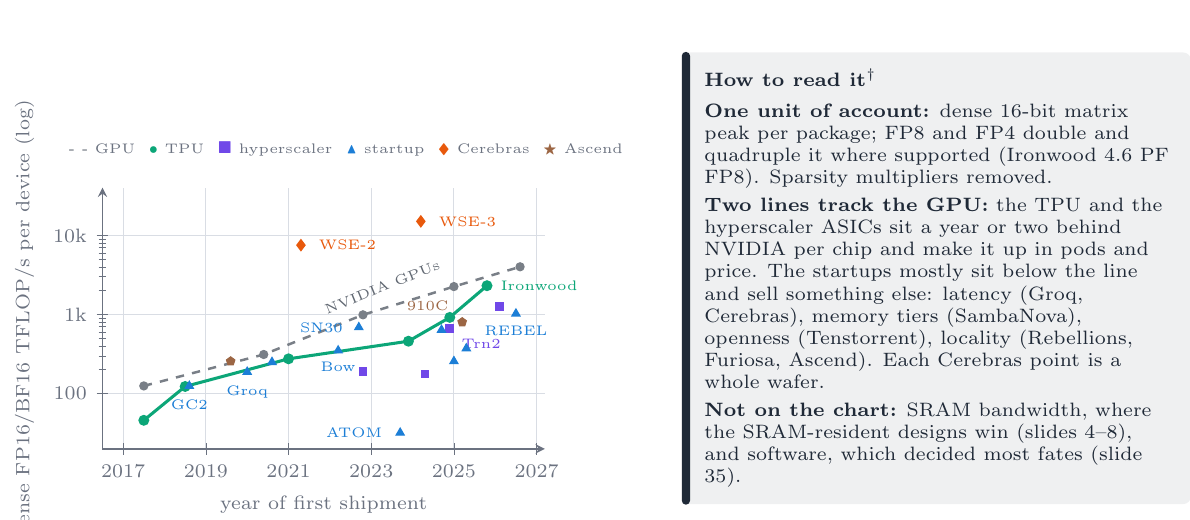
\begin{tikzpicture}
  \useasboundingbox (0,0) rectangle (14.4,5.9);
  \begin{scope}[shift={(0.95,0.55)}]
  \begin{axis}[lecture,width=7.2cm,height=4.9cm,ymode=log,xmin=2016.5,xmax=2027.2,ymin=20,ymax=40000,
      xlabel={year of first shipment},ylabel={dense FP16/BF16 TFLOP/s per device (log)},
      xtick={2017,2019,2021,2023,2025,2027},xticklabel style={/pgf/number format/1000 sep={}},scaled x ticks=false,
      ytick={100,1000,10000},yticklabels={100,1k,10k},
      title style={font=\tiny,text=muted,at={(0.55,1.02)}},title={\textcolor{ink!70}{- -} GPU \ \textcolor{emb}{$\bullet$} TPU \ \textcolor{posc}{$\blacksquare$} hyperscaler \ \textcolor{mlp}{$\blacktriangle$} startup \ \textcolor{attn}{$\blacklozenge$} Cerebras \ \textcolor{trn}{$\bigstar$} Ascend}]
    \addplot[ink!60,dashed,line width=0.9pt,mark=*,mark size=1.2pt,mark options={solid}] coordinates {(2017.5,125) (2020.4,312) (2022.8,989) (2025.0,2250) (2026.6,4000)};
    \addplot[emb,line width=1.1pt,mark=*,mark size=1.4pt] coordinates {(2017.5,46) (2018.5,123) (2021.0,275) (2023.9,459) (2024.9,918) (2025.8,2307)};
    \addplot[posc,only marks,mark=square*,mark size=1.4pt] coordinates {(2022.8,190) (2024.9,667) (2024.3,177) (2026.1,1270)};
    \addplot[mlp,only marks,mark=triangle*,mark size=1.7pt] coordinates {(2018.6,125) (2020.6,250) (2022.2,350) (2020.0,188) (2022.7,688) (2024.7,638) (2025.3,372) (2023.7,32) (2025.0,256) (2026.5,1024)};
    \addplot[attn,only marks,mark=diamond*,mark size=2pt] coordinates {(2021.3,7500) (2024.2,15000)};
    \addplot[trn,only marks,mark=pentagon*,mark size=1.6pt] coordinates {(2019.6,256) (2025.2,800)};
    \node[font=\tiny,text=attn,anchor=west] at (axis cs:2024.4,15000) {WSE-3};
    \node[font=\tiny,text=ink!70,anchor=south,rotate=22] at (axis cs:2023.4,1500) {NVIDIA GPUs};
    \node[font=\tiny,text=posc,anchor=north west] at (axis cs:2024.95,640) {Trn2};
    \node[font=\tiny,text=mlp,anchor=north] at (axis cs:2022.2,330) {Bow};
    \node[font=\tiny,text=attn,anchor=west] at (axis cs:2021.5,7500) {WSE-2};
    \node[font=\tiny,text=mlp,anchor=east] at (axis cs:2023.5,32) {ATOM};
    \node[font=\tiny,text=mlp,anchor=north] at (axis cs:2026.5,960) {REBEL};
    \node[font=\tiny,text=mlp,anchor=north] at (axis cs:2020.0,165) {Groq};
    \node[font=\tiny,text=mlp,anchor=east] at (axis cs:2022.55,688) {SN30};
    \node[font=\tiny,text=mlp,anchor=north] at (axis cs:2018.6,110) {GC2};
    \node[font=\tiny,text=emb,anchor=west] at (axis cs:2025.9,2307) {Ironwood};
    \node[font=\tiny,text=trn,anchor=south east] at (axis cs:2025.1,850) {910C};
  \end{axis}
  \end{scope}
  \bgpanels{8.3}{5.6}{5.9cm}{How to read it$^\dagger$}{%
    \hl{ink}{One unit of account:} dense 16-bit matrix peak per
    package; FP8 and FP4 double and quadruple it where supported
    (Ironwood 4.6 PF FP8). Sparsity multipliers removed.\\[2pt]
    \hl{ink}{Two lines track the GPU:} the TPU and the hyperscaler
    ASICs sit a year or two behind NVIDIA per chip and make it up in
    pods and price. The startups mostly sit below the line and sell
    something else: latency (Groq, Cerebras), memory tiers
    (SambaNova), openness (Tenstorrent), locality (Rebellions,
    Furiosa, Ascend). Each Cerebras point is a whole wafer.\\[2pt]
    \hl{ink}{Not on the chart:} SRAM bandwidth, where the
    SRAM-resident designs win (slides 4--8), and software, which
    decided most fates (slide 35).}
\end{tikzpicture}
\end{frame}

% ---------------------------------------------------------------- 3
\begin{frame}{Who is who: fifteen programs, 2016--2027}
\framesubtitle{First and latest chips, the design idea, and where each program stood in November 2026.}
\centering
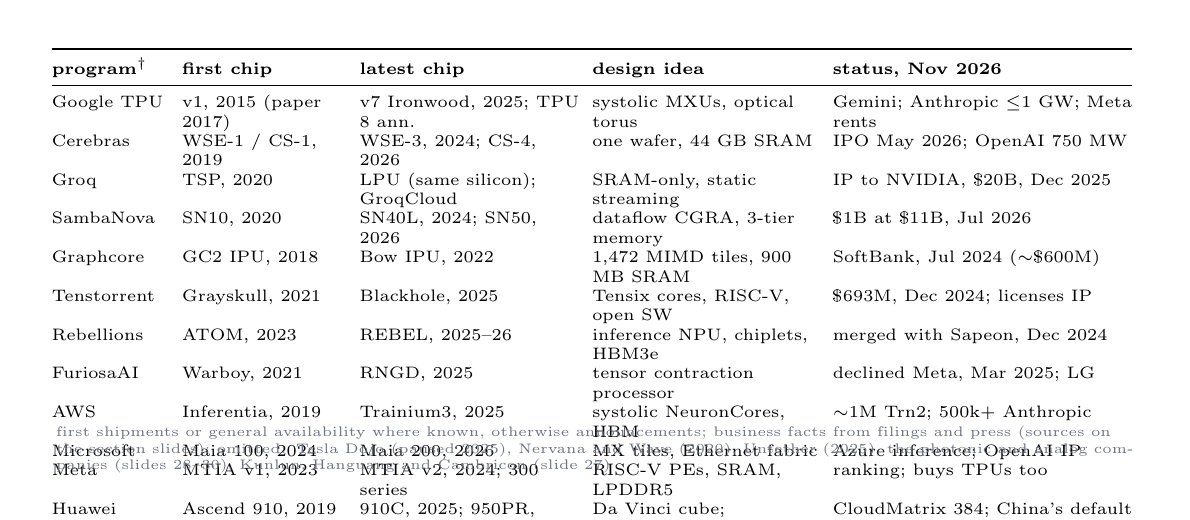
\begin{tikzpicture}
  \useasboundingbox (0,0) rectangle (14.4,5.9);
  \node[anchor=north west,inner sep=0,font=\fontsize{6.0}{7.0}\selectfont] at (0.3,5.65) {%
    \renewcommand{\arraystretch}{1.0}\setlength{\tabcolsep}{2.2pt}%
    \begin{tabular}{@{}>{\raggedright\arraybackslash}p{1.5cm}>{\raggedright\arraybackslash}p{2.1cm}>{\raggedright\arraybackslash}p{2.8cm}>{\raggedright\arraybackslash}p{2.9cm}>{\raggedright\arraybackslash}p{3.8cm}@{}}
      \toprule
      \textbf{program}$^\dagger$ & \textbf{first chip} & \textbf{latest chip} & \textbf{design idea} & \textbf{status, Nov 2026}\\
      \midrule
      Google TPU & v1, 2015 (paper 2017) & v7 Ironwood, 2025; TPU 8 ann. & systolic MXUs, optical torus & Gemini; Anthropic $\le$1 GW; Meta rents\\
      Cerebras & WSE-1 / CS-1, 2019 & WSE-3, 2024; CS-4, 2026 & one wafer, 44 GB SRAM & IPO May 2026; OpenAI 750 MW\\
      Groq & TSP, 2020 & LPU (same silicon); GroqCloud & SRAM-only, static streaming & IP to NVIDIA, \$20B, Dec 2025\\
      SambaNova & SN10, 2020 & SN40L, 2024; SN50, 2026 & dataflow CGRA, 3-tier memory & \$1B at \$11B, Jul 2026\\
      Graphcore & GC2 IPU, 2018 & Bow IPU, 2022 & 1{,}472 MIMD tiles, 900 MB SRAM & SoftBank, Jul 2024 (${\sim}$\$600M)\\
      Tenstorrent & Grayskull, 2021 & Blackhole, 2025 & Tensix cores, RISC-V, open SW & \$693M, Dec 2024; licenses IP\\
      Rebellions & ATOM, 2023 & REBEL, 2025--26 & inference NPU, chiplets, HBM3e & merged with Sapeon, Dec 2024\\
      FuriosaAI & Warboy, 2021 & RNGD, 2025 & tensor contraction processor & declined Meta, Mar 2025; LG\\
      AWS & Inferentia, 2019 & Trainium3, 2025 & systolic NeuronCores, HBM & ${\sim}$1M Trn2; 500k$+$ Anthropic\\
      Microsoft & Maia 100, 2024 & Maia 200, 2026 & MX tiles, Ethernet fabric & Azure inference; OpenAI IP\\
      Meta & MTIA v1, 2023 & MTIA v2, 2024; 300 series & RISC-V PEs, SRAM, LPDDR5 & ranking; buys TPUs too\\
      Huawei & Ascend 910, 2019 & 910C, 2025; 950PR, 2026 & Da Vinci cube; SuperPoDs & CloudMatrix 384; China's default\\
      Intel Habana & Gaudi, 2019 & Gaudi 3, 2024 & MME $+$ TPCs, Ethernet on chip & line ended 2025\\
      Qualcomm & Cloud AI 100, 2021 & AI200, 2026; AI250, 2027 & NPU cores, LPDDR capacity & 200 MW with Humain\\
      d-Matrix & Corsair, 2024 & Raptor, 2026 & digital in-memory compute & \$275M at \$2B, Nov 2025\\
      \bottomrule
    \end{tabular}};
  \node[lab,anchor=north west,text width=13.8cm,font=\tiny] at (0.3,0.9) {first shipments or general availability where known, otherwise announcements; business facts from filings and press (sources on the section slides); omitted: Tesla Dojo (paused 2025), Nervana and Wave (2020), Untether (2025), the photonic and analog companies (slides 28--30), Kunlun, Hanguang and Cambricon (slide 27)};
\end{tikzpicture}
\end{frame}

% ---------------------------------------------------------------- 4
\stage{2}
\begin{frame}{The memory wall: why the GPU's critics had a point}
\framesubtitle{Peak compute grew 3$\times$ every two years, DRAM bandwidth 1.6$\times$, interconnect 1.4$\times$; decode is bandwidth-bound.}
\centering
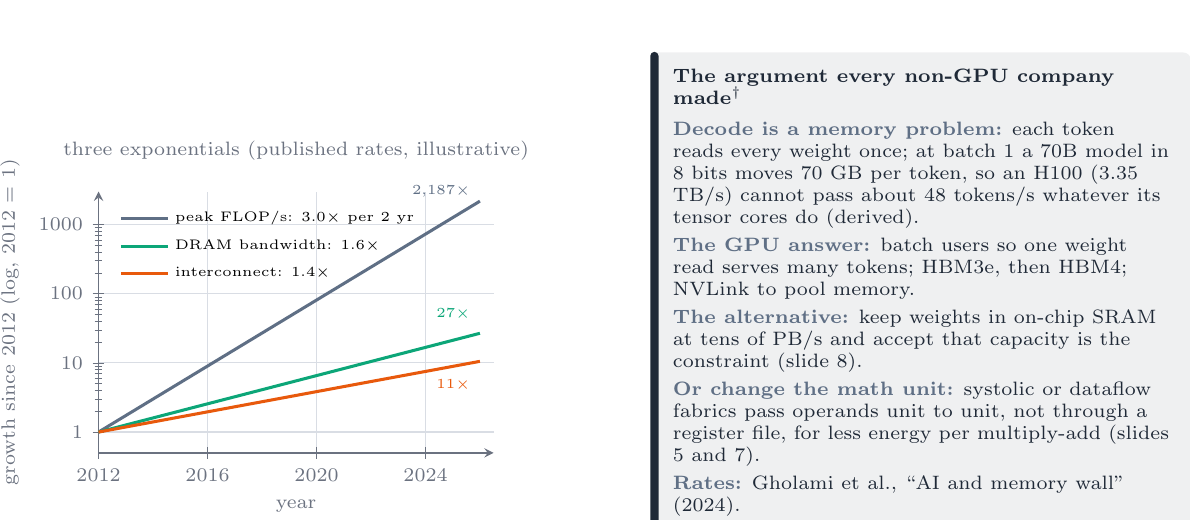
\begin{tikzpicture}
  \useasboundingbox (0,0) rectangle (14.4,5.9);
  \begin{scope}[shift={(0.9,0.5)}]
  \begin{axis}[lecture,width=6.6cm,height=4.9cm,ymode=log,xmin=2012,xmax=2026.5,ymin=0.5,ymax=3000,
      xlabel={year},ylabel={growth since 2012 (log, 2012 $=$ 1)},
      xtick={2012,2016,2020,2024},xticklabel style={/pgf/number format/1000 sep={}},scaled x ticks=false,
      ytick={1,10,100,1000},yticklabels={1,10,100,1000},
      legend style={at={(0.03,0.97)},anchor=north west,font=\tiny},
      title style={font=\scriptsize,text=muted,at={(0.5,1.02)}},title={three exponentials (published rates, illustrative)}]
    \addplot[tok,line width=1.1pt,domain=2012:2026,samples=30] {3^((x-2012)/2)};
    \addlegendentry{peak FLOP/s: 3.0$\times$ per 2 yr}
    \addplot[emb,line width=1.1pt,domain=2012:2026,samples=30] {1.6^((x-2012)/2)};
    \addlegendentry{DRAM bandwidth: 1.6$\times$}
    \addplot[attn,line width=1.1pt,domain=2012:2026,samples=30] {1.4^((x-2012)/2)};
    \addlegendentry{interconnect: 1.4$\times$}
    \node[font=\tiny,text=tok,anchor=south east] at (axis cs:2026,1800) {2{,}187$\times$};
    \node[font=\tiny,text=emb,anchor=south east] at (axis cs:2026,30) {27$\times$};
    \node[font=\tiny,text=attn,anchor=north east] at (axis cs:2026,8) {11$\times$};
  \end{axis}
  \end{scope}
  \bgpanels{7.9}{5.6}{6.3cm}{The argument every non-GPU company made$^\dagger$}{%
    \hl{tok}{Decode is a memory problem:} each token reads every
    weight once; at batch 1 a 70B model in 8 bits moves 70 GB per
    token, so an H100 (3.35 TB/s) cannot pass about 48 tokens/s
    whatever its tensor cores do (derived).\\[2pt]
    \hl{tok}{The GPU answer:} batch users so one weight read serves
    many tokens; HBM3e, then HBM4; NVLink to pool memory.\\[2pt]
    \hl{tok}{The alternative:} keep weights in on-chip SRAM at tens
    of PB/s and accept that capacity is the constraint (slide 8).\\[2pt]
    \hl{tok}{Or change the math unit:} systolic or dataflow fabrics
    pass operands unit to unit, not through a register file, for less
    energy per multiply-add (slides 5 and 7).\\[2pt]
    \hl{tok}{Rates:} Gholami et al., ``AI and memory wall'' (2024).}
\end{tikzpicture}
\end{frame}

% ---------------------------------------------------------------- 5
\begin{frame}{A taxonomy: five ways to organize a tensor machine}
\framesubtitle{Where the operands wait and who decides when they move: in hardware, in a compiler schedule, or in a program.}
\centering
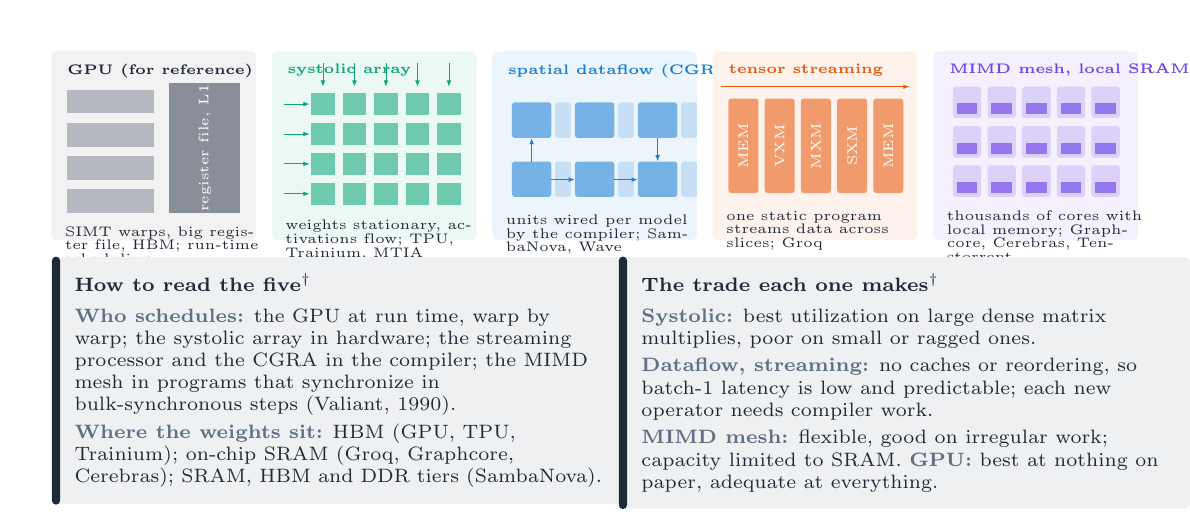
\begin{tikzpicture}
  \useasboundingbox (0,0) rectangle (14.4,5.9);
  % five mini-diagrams across the top, labels below
  % 1 SIMT GPU
  \begin{scope}[shift={(0.3,3.2)}]
    \fill[ink!6,rounded corners=2pt] (0,0) rectangle (2.6,2.4);
    \node[font=\fontsize{5.5}{6}\selectfont\bfseries,text=ink,anchor=north west] at (0.08,2.36) {GPU (for reference)};
    \foreach \r in {0,1,2,3}{\fill[muted!50] (0.2,0.35+\r*0.42) rectangle (1.3,0.35+\r*0.42+0.3);}
    \fill[muted!80] (1.5,0.35) rectangle (2.4,2.0);
    \node[font=\fontsize{4.2}{5}\selectfont,text=white,rotate=90] at (1.95,1.17) {register file, L1};
    \node[font=\fontsize{4.2}{5}\selectfont,text=ink,anchor=north west,text width=2.5cm] at (0.05,0.3) {SIMT warps, big register file, HBM; run-time scheduling};
  \end{scope}
  % 2 systolic
  \begin{scope}[shift={(3.1,3.2)}]
    \fill[emb!8,rounded corners=2pt] (0,0) rectangle (2.6,2.4);
    \node[font=\fontsize{5.5}{6}\selectfont\bfseries,text=emb,anchor=north west] at (0.08,2.36) {systolic array};
    \foreach \c in {0,...,4}{\foreach \r in {0,...,3}{\fill[emb!60] (0.5+\c*0.4,0.45+\r*0.38) rectangle ++(0.3,0.28);}}
    \foreach \r in {0,...,3}{\draw[emb,-{Latex[length=0.8mm]},line width=0.3pt] (0.15,0.59+\r*0.38) -- (0.48,0.59+\r*0.38);}
    \foreach \c in {0,...,4}{\draw[emb,-{Latex[length=0.8mm]},line width=0.3pt] (0.65+\c*0.4,2.25) -- (0.65+\c*0.4,1.95);}
    \node[font=\fontsize{4.2}{5}\selectfont,text=ink,anchor=north west,text width=2.5cm] at (0.05,0.38) {weights stationary, activations flow; TPU, Trainium, MTIA};
  \end{scope}
  % 3 spatial dataflow / CGRA
  \begin{scope}[shift={(5.9,3.2)}]
    \fill[mlp!8,rounded corners=2pt] (0,0) rectangle (2.6,2.4);
    \node[font=\fontsize{5.5}{6}\selectfont\bfseries,text=mlp,anchor=north west] at (0.08,2.36) {spatial dataflow (CGRA)};
    \foreach \c in {0,1,2}{\foreach \r in {0,1}{\fill[mlp!60,rounded corners=1pt] (0.25+\c*0.8,0.55+\r*0.75) rectangle ++(0.5,0.45);
      \fill[mlp!25,rounded corners=1pt] (0.25+\c*0.8+0.55,0.55+\r*0.75) rectangle ++(0.2,0.45);}}
    \draw[mlp,-{Latex[length=0.8mm]},line width=0.4pt] (0.75,0.77) -- (1.05,0.77);
    \draw[mlp,-{Latex[length=0.8mm]},line width=0.4pt] (1.55,0.77) -- (1.85,0.77);
    \draw[mlp,-{Latex[length=0.8mm]},line width=0.4pt] (0.5,1.0) -- (0.5,1.3);
    \draw[mlp,-{Latex[length=0.8mm]},line width=0.4pt] (2.1,1.3) -- (2.1,1.0);
    \node[font=\fontsize{4.2}{5}\selectfont,text=ink,anchor=north west,text width=2.5cm] at (0.05,0.45) {units wired per model by the compiler; SambaNova, Wave};
  \end{scope}
  % 4 tensor streaming / VLIW deterministic
  \begin{scope}[shift={(8.7,3.2)}]
    \fill[attn!8,rounded corners=2pt] (0,0) rectangle (2.6,2.4);
    \node[font=\fontsize{5.5}{6}\selectfont\bfseries,text=attn,anchor=north west] at (0.08,2.36) {tensor streaming};
    \foreach \c/\lab in {0/MEM,1/VXM,2/MXM,3/SXM,4/MEM}{\fill[attn!60,rounded corners=1pt] (0.2+\c*0.46,0.6) rectangle ++(0.38,1.2);
      \node[font=\fontsize{3.6}{4}\selectfont,text=white,rotate=90] at (0.39+\c*0.46,1.2) {\lab};}
    \draw[attn,-{Latex[length=0.8mm]},line width=0.5pt] (0.1,1.95) -- (2.5,1.95);
    \node[font=\fontsize{4.2}{5}\selectfont,text=ink,anchor=north west,text width=2.5cm] at (0.05,0.5) {one static program streams data across slices; Groq};
  \end{scope}
  % 5 BSP MIMD distributed SRAM / wafer
  \begin{scope}[shift={(11.5,3.2)}]
    \fill[posc!8,rounded corners=2pt] (0,0) rectangle (2.6,2.4);
    \node[font=\fontsize{5.5}{6}\selectfont\bfseries,text=posc,anchor=north west] at (0.08,2.36) {MIMD mesh, local SRAM};
    \foreach \c in {0,...,4}{\foreach \r in {0,...,2}{\fill[posc!25,rounded corners=1pt] (0.25+\c*0.44,0.55+\r*0.5) rectangle ++(0.36,0.4); \fill[posc!75] (0.3+\c*0.44,0.6+\r*0.5) rectangle ++(0.26,0.14);}}
    \node[font=\fontsize{4.2}{5}\selectfont,text=ink,anchor=north west,text width=2.5cm] at (0.05,0.5) {thousands of cores with local memory; Graphcore, Cerebras, Tenstorrent};
  \end{scope}
  \bgpanels{0.3}{3.0}{6.7cm}{How to read the five$^\dagger$}{%
    \hl{tok}{Who schedules:} the GPU at run time, warp by warp; the
    systolic array in hardware; the streaming processor and the CGRA
    in the compiler; the MIMD mesh in programs that synchronize in
    bulk-synchronous steps (Valiant, 1990).\\[2pt]
    \hl{tok}{Where the weights sit:} HBM (GPU, TPU, Trainium); on-chip
    SRAM (Groq, Graphcore, Cerebras); SRAM, HBM and DDR tiers
    (SambaNova).}
  \bgpanels{7.5}{3.0}{6.7cm}{The trade each one makes$^\dagger$}{%
    \hl{tok}{Systolic:} best utilization on large dense matrix
    multiplies, poor on small or ragged ones.\\[2pt]
    \hl{tok}{Dataflow, streaming:} no caches or reordering, so batch-1
    latency is low and predictable; each new operator needs compiler
    work.\\[2pt]
    \hl{tok}{MIMD mesh:} flexible, good on irregular work; capacity
    limited to SRAM. \hl{tok}{GPU:} best at nothing on paper,
    adequate at everything.}
\end{tikzpicture}
\end{frame}


% ---------------------------------------------------------------- 6
\begin{frame}{Why not a GPU? What a special-purpose chip gives up}
\framesubtitle{TPU v1 (2017): 15--30$\times$ a K80 and 30--80$\times$ its perf/W, by dropping what a GPU keeps.}
\centering
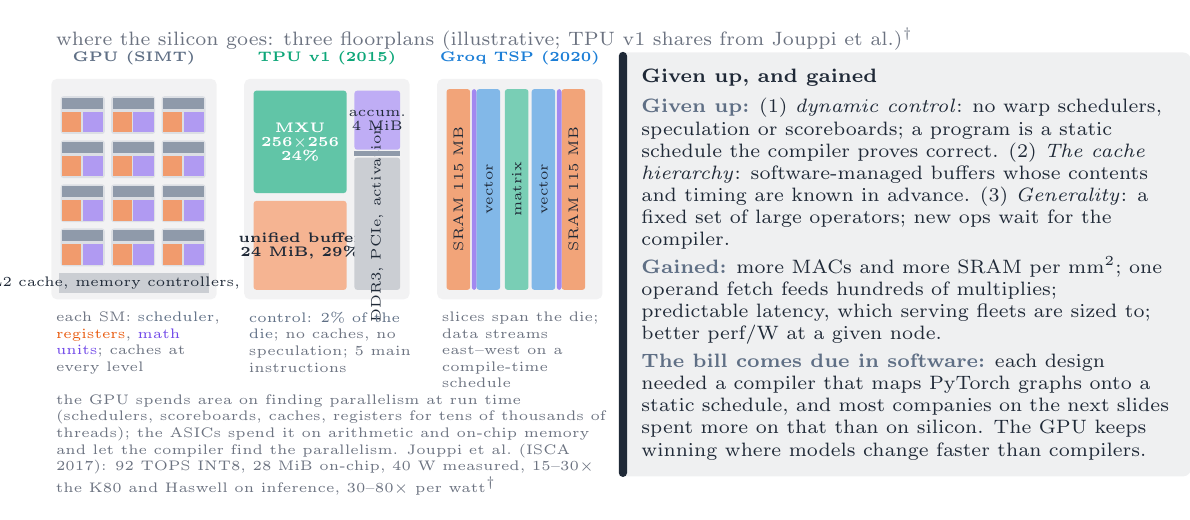
\begin{tikzpicture}
  \useasboundingbox (0,0) rectangle (14.4,5.9);
  \node[lab,anchor=south west] at (0.3,5.55) {where the silicon goes: three floorplans (illustrative; TPU v1 shares from Jouppi et al.)$^\dagger$};
  % --- GPU die
  \begin{scope}[shift={(0.3,2.45)}]
    \fill[ink!6,rounded corners=2pt] (0,0) rectangle (2.1,2.8);
    \foreach \r in {0,1,2,3}{\foreach \c in {0,1,2}{
      \fill[tok!22,rounded corners=1pt] (0.12+\c*0.64,0.42+\r*0.56) rectangle ++(0.56,0.48);
      \fill[tok!70] (0.14+\c*0.64,0.74+\r*0.56) rectangle ++(0.52,0.14);
      \fill[attn!60] (0.14+\c*0.64,0.44+\r*0.56) rectangle ++(0.24,0.26);
      \fill[posc!55] (0.4+\c*0.64,0.44+\r*0.56) rectangle ++(0.26,0.26);}}
    \fill[muted!35] (0.1,0.08) rectangle (2.0,0.34);
    \node[font=\fontsize{4.2}{5}\selectfont,text=ink] at (1.05,0.21) {L2 cache, memory controllers, I/O};
    \node[font=\fontsize{5}{6}\selectfont\bfseries,text=tok,anchor=south] at (1.05,2.85) {GPU (SIMT)};
  \end{scope}
  \node[lab,font=\tiny,anchor=north west,text width=2.2cm,align=flush left] at (0.3,2.35) {each SM: \textcolor{tok}{scheduler}, \textcolor{attn}{registers}, \textcolor{posc}{math units}; caches at every level};
  % --- TPU v1 die
  \begin{scope}[shift={(2.75,2.45)}]
    \fill[ink!6,rounded corners=2pt] (0,0) rectangle (2.1,2.8);
    \fill[emb!65,rounded corners=1pt] (0.12,1.35) rectangle (1.3,2.65);
    \node[font=\fontsize{4.4}{5}\selectfont\bfseries,text=white,align=center] at (0.71,2.0) {MXU\\256$\times$256\\24\%};
    \fill[attn!45,rounded corners=1pt] (0.12,0.12) rectangle (1.3,1.25);
    \node[font=\fontsize{4.4}{5}\selectfont\bfseries,text=ink,align=center] at (0.71,0.68) {unified buffer\\24 MiB, 29\%};
    \fill[posc!45,rounded corners=1pt] (1.4,1.9) rectangle (1.98,2.65);
    \node[font=\fontsize{4}{5}\selectfont,text=ink,align=center] at (1.69,2.27) {accum.\\4 MiB};
    \fill[muted!35,rounded corners=1pt] (1.4,0.12) rectangle (1.98,1.8);
    \node[font=\fontsize{4}{5}\selectfont,text=ink,align=center,rotate=90] at (1.69,0.96) {DDR3, PCIe, activation};
    \fill[tok!70] (1.4,1.82) rectangle (1.98,1.88);
    \node[font=\fontsize{5}{6}\selectfont\bfseries,text=emb,anchor=south] at (1.05,2.85) {TPU v1 (2015)};
  \end{scope}
  \node[lab,font=\tiny,anchor=north west,text width=2.2cm,align=flush left] at (2.75,2.35) {\textcolor{tok}{control: 2\% of the die}; no caches, no speculation; 5 main instructions};
  % --- Groq die
  \begin{scope}[shift={(5.2,2.45)}]
    \fill[ink!6,rounded corners=2pt] (0,0) rectangle (2.1,2.8);
    \foreach \x/\c in {0.12/attn,0.5/mlp,0.86/emb,1.2/mlp,1.58/attn}{\fill[\c!55,rounded corners=1pt] (\x,0.12) rectangle ++(0.3,2.55);}
    \fill[posc!65,rounded corners=1pt] (0.44,0.12) rectangle (0.5,2.67); \fill[posc!65,rounded corners=1pt] (1.52,0.12) rectangle (1.58,2.67);
    \node[font=\fontsize{4}{5}\selectfont,text=ink,rotate=90] at (0.27,1.4) {SRAM 115 MB};
    \node[font=\fontsize{4}{5}\selectfont,text=ink,rotate=90] at (1.73,1.4) {SRAM 115 MB};
    \node[font=\fontsize{4}{5}\selectfont,text=ink,rotate=90] at (0.65,1.4) {vector};
    \node[font=\fontsize{4}{5}\selectfont,text=ink,rotate=90] at (1.01,1.4) {matrix};
    \node[font=\fontsize{4}{5}\selectfont,text=ink,rotate=90] at (1.35,1.4) {vector};
    \node[font=\fontsize{5}{6}\selectfont\bfseries,text=mlp,anchor=south] at (1.05,2.85) {Groq TSP (2020)};
  \end{scope}
  \node[lab,font=\tiny,anchor=north west,text width=2.2cm,align=flush left] at (5.2,2.35) {slices span the die; data streams east--west on a compile-time schedule};
  \node[lab,font=\tiny,anchor=north west,text width=7.0cm,align=flush left] at (0.3,1.3) {the GPU spends area on finding parallelism at run time (schedulers, scoreboards, caches, registers for tens of thousands of threads); the ASICs spend it on arithmetic and on-chip memory and let the compiler find the parallelism. Jouppi et al.\ (ISCA 2017): 92 TOPS INT8, 28 MiB on-chip, 40 W measured, 15--30$\times$ the K80 and Haswell on inference, 30--80$\times$ per watt$^\dagger$};
  \bgpanels{7.5}{5.6}{6.7cm}{Given up, and gained}{%
    \hl{tok}{Given up:} (1) \emph{dynamic control}: no warp schedulers,
    speculation or scoreboards; a program is a static schedule the
    compiler proves correct. (2) \emph{The cache hierarchy}:
    software-managed buffers whose contents and timing are known in
    advance. (3) \emph{Generality}: a fixed set of large operators;
    new ops wait for the compiler.\\[2pt]
    \hl{tok}{Gained:} more MACs and more SRAM per mm$^2$; one operand
    fetch feeds hundreds of multiplies; predictable latency, which
    serving fleets are sized to; better perf/W at a given node.\\[2pt]
    \hl{tok}{The bill comes due in software:} each design needed a
    compiler that maps PyTorch graphs onto a static schedule, and
    most companies on the next slides spent more on that than on
    silicon. The GPU keeps winning where models change faster than
    compilers.}
\end{tikzpicture}
\end{frame}

% ---------------------------------------------------------------- 7
\begin{frame}{Systolic arrays and the MXU: reuse by geometry}
\framesubtitle{16,384 multiply-adds per clock from one operand read per row; the TPU has kept the idea for seven generations.}
\centering
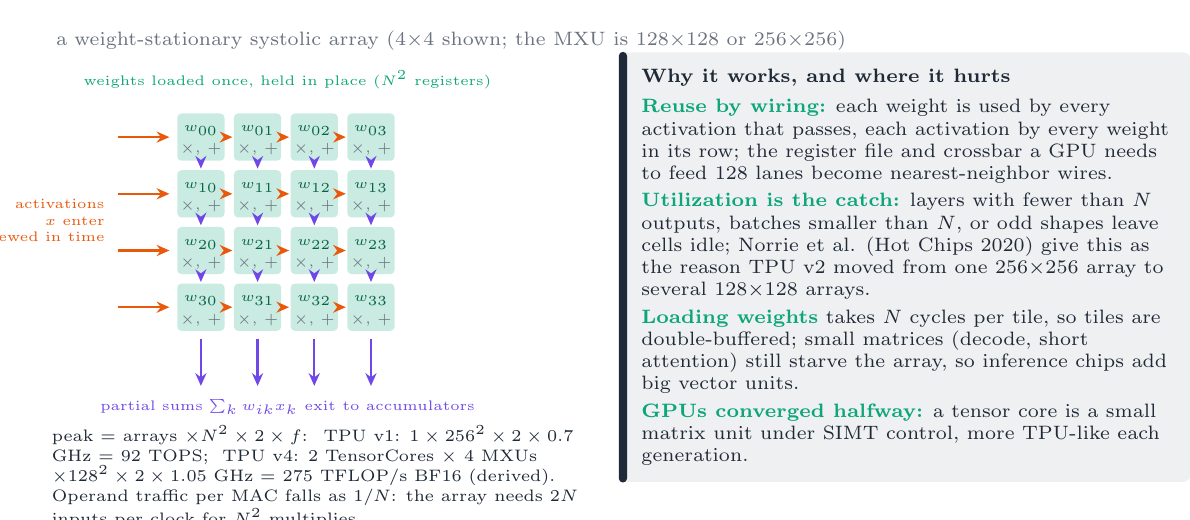
\begin{tikzpicture}
  \useasboundingbox (0,0) rectangle (14.4,5.9);
  \node[lab,anchor=south west] at (0.3,5.55) {a weight-stationary systolic array (4$\times$4 shown; the MXU is 128$\times$128 or 256$\times$256)};
  \begin{scope}[shift={(1.9,2.05)}]
    \foreach \r in {0,...,3}{\pgfmathtruncatemacro{\rr}{3-\r}\foreach \c in {0,...,3}{
      \fill[emb!22,rounded corners=1.5pt] (\c*0.72,\r*0.72) rectangle ++(0.6,0.6);
      \node[font=\fontsize{4.6}{5}\selectfont,text=emb!60!black] at (\c*0.72+0.3,\r*0.72+0.38) {$w_{\rr\c}$};
      \node[font=\fontsize{3.8}{4}\selectfont,text=muted] at (\c*0.72+0.3,\r*0.72+0.14) {$\times$, $+$};}}
    % activations flow left to right
    \foreach \r in {0,...,3}{\draw[flow,attn] (-0.75,\r*0.72+0.3) -- (-0.1,\r*0.72+0.3);
      \foreach \c in {0,1,2}{\draw[thinflow,attn] (\c*0.72+0.62,\r*0.72+0.3) -- (\c*0.72+0.7,\r*0.72+0.3);}}
    \node[font=\tiny,text=attn,anchor=east,align=right] at (-0.8,1.4) {activations\\$x$ enter\\skewed in time};
    % partial sums flow down
    \foreach \c in {0,...,3}{\draw[flow,posc] (\c*0.72+0.3,-0.1) -- (\c*0.72+0.3,-0.7);
      \foreach \r in {1,2,3}{\draw[thinflow,posc] (\c*0.72+0.3,\r*0.72-0.02) -- (\c*0.72+0.3,\r*0.72-0.1);}}
    \node[font=\tiny,text=posc,anchor=north] at (1.4,-0.75) {partial sums $\sum_k w_{ik}x_k$ exit to accumulators};
    \node[font=\tiny,text=emb,anchor=south] at (1.4,2.95) {weights loaded once, held in place ($N^2$ registers)};
  \end{scope}
  \node[anchor=north west,inner sep=0,font=\fontsize{6}{7.2}\selectfont,text=ink,text width=6.9cm,align=flush left] at (0.3,0.85) {%
    peak $=$ arrays $\times N^2 \times 2 \times f$: \ TPU v1: $1\times256^2\times2\times0.7$ GHz $=$ 92 TOPS; \ TPU v4: 2 TensorCores $\times$ 4 MXUs $\times 128^2 \times 2 \times 1.05$ GHz $=$ 275 TFLOP/s BF16 (derived). Operand traffic per MAC falls as $1/N$: the array needs $2N$ inputs per clock for $N^2$ multiplies.};
  \bgpanels{7.5}{5.6}{6.7cm}{Why it works, and where it hurts}{%
    \hl{emb}{Reuse by wiring:} each weight is used by every
    activation that passes, each activation by every weight in its
    row; the register file and crossbar a GPU needs to feed 128
    lanes become nearest-neighbor wires.\\[2pt]
    \hl{emb}{Utilization is the catch:} layers with fewer than $N$
    outputs, batches smaller than $N$, or odd shapes leave cells
    idle; Norrie et al. (Hot Chips 2020) give this as the reason
    TPU v2 moved from one 256$\times$256 array to several
    128$\times$128 arrays.\\[2pt]
    \hl{emb}{Loading weights} takes $N$ cycles per tile, so tiles
    are double-buffered; small matrices (decode, short attention)
    still starve the array, so inference chips add big vector units.\\[2pt]
    \hl{emb}{GPUs converged halfway:} a tensor core is a small
    matrix unit under SIMT control, more TPU-like each generation.}
\end{tikzpicture}
\end{frame}


% ---------------------------------------------------------------- 8
\begin{frame}{SRAM against HBM: bandwidth is cheap on chip, capacity isn't}
\framesubtitle{An on-chip read costs a hundredth of a DRAM access; a 70B model on chip takes hundreds of chips or a wafer.}
\centering
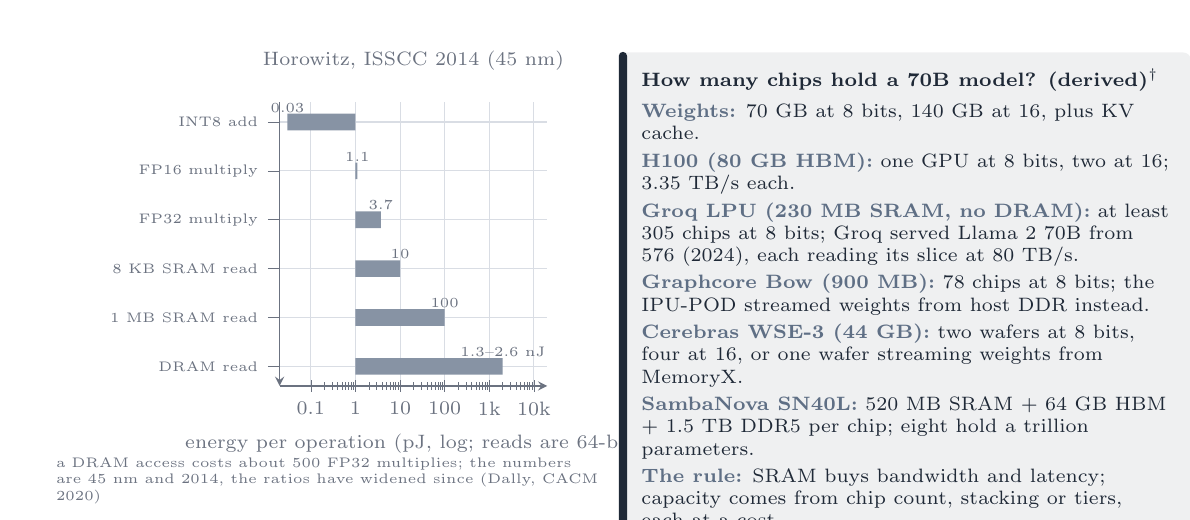
\begin{tikzpicture}
  \useasboundingbox (0,0) rectangle (14.4,5.9);
  \begin{scope}[shift={(3.2,1.35)}]
  \begin{axis}[lecture,scale only axis,width=3.4cm,height=3.6cm,xbar,bar width=6pt,xmode=log,xmin=0.02,xmax=20000,enlarge y limits=0.08,
      symbolic y coords={{INT8 add},{FP16 multiply},{FP32 multiply},{8 KB SRAM read},{1 MB SRAM read},{DRAM read}},
      ytick=data,y dir=reverse,yticklabel style={font=\tiny},xlabel={energy per operation (pJ, log; reads are 64-bit)},
      xtick={0.1,1,10,100,1000,10000},xticklabels={0.1,1,10,100,1k,10k},
      nodes near coords,nodes near coords style={font=\tiny,text=muted},point meta=explicit symbolic,
      title style={font=\scriptsize,text=muted,at={(0.5,1.02)}},title={Horowitz, ISSCC 2014 (45 nm)}]
    \addplot[fill=tok!75,draw=none] coordinates {(0.03,{INT8 add})[0.03] (1.1,{FP16 multiply})[1.1] (3.7,{FP32 multiply})[3.7] (10,{8 KB SRAM read})[10] (100,{1 MB SRAM read})[100] (2000,{DRAM read})[1.3--2.6 nJ]};
  \end{axis}
  \end{scope}
  \node[lab,font=\tiny,anchor=north west,text width=6.9cm] at (0.3,0.5) {a DRAM access costs about 500 FP32 multiplies; the numbers are 45 nm and 2014, the ratios have widened since (Dally, CACM 2020)};
  \bgpanels{7.5}{5.6}{6.7cm}{How many chips hold a 70B model? (derived)$^\dagger$}{%
    \hl{tok}{Weights:} 70 GB at 8 bits, 140 GB at 16, plus KV cache.\\[2pt]
    \hl{tok}{H100 (80 GB HBM):} one GPU at 8 bits, two at 16; 3.35
    TB/s each.\\[2pt]
    \hl{tok}{Groq LPU (230 MB SRAM, no DRAM):} at least 305 chips at
    8 bits; Groq served Llama 2 70B from 576 (2024), each reading its
    slice at 80 TB/s.\\[2pt]
    \hl{tok}{Graphcore Bow (900 MB):} 78 chips at 8 bits; the IPU-POD
    streamed weights from host DDR instead.\\[2pt]
    \hl{tok}{Cerebras WSE-3 (44 GB):} two wafers at 8 bits, four at
    16, or one wafer streaming weights from MemoryX.\\[2pt]
    \hl{tok}{SambaNova SN40L:} 520 MB SRAM $+$ 64 GB HBM $+$ 1.5 TB
    DDR5 per chip; eight hold a trillion parameters.\\[2pt]
    \hl{tok}{The rule:} SRAM buys bandwidth and latency; capacity
    comes from chip count, stacking or tiers, each at a cost.}
\end{tikzpicture}
\end{frame}

% ---------------------------------------------------------------- 9
\stage{3}
\begin{frame}{Google TPU v1 to v3: the systolic array goes to the data center}
\framesubtitle{A 2015 inference coprocessor became, by 2018, a liquid-cooled 1,024-chip training pod; the pod is the design unit.}
\centering
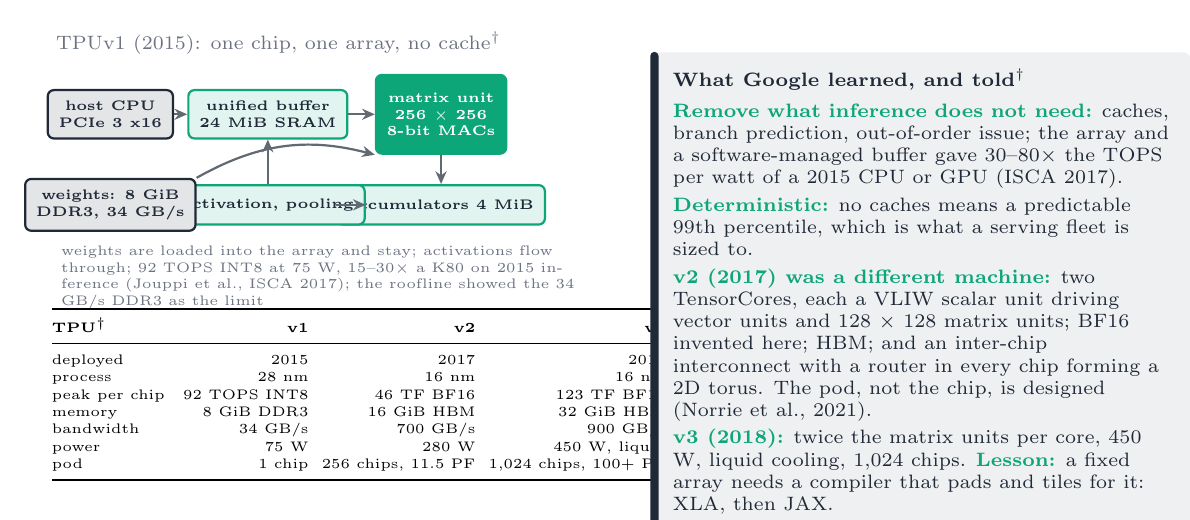
\begin{tikzpicture}
  \useasboundingbox (0,0) rectangle (14.4,5.9);
  % TPUv1 block diagram
  \node[lab,anchor=south west] at (0.3,5.5) {TPUv1 (2015): one chip, one array, no cache$^\dagger$};
  \begin{scope}[shift={(0.3,2.9)}]
    \node[comp=ink,minimum width=1.3cm,minimum height=0.55cm,font=\fontsize{5}{6}\selectfont\bfseries,text=ink,align=center] (host) at (0.75,1.9) {host CPU\\PCIe 3 x16};
    \node[comp=emb,minimum width=1.6cm,minimum height=0.55cm,font=\fontsize{5}{6}\selectfont\bfseries,text=ink,align=center] (ub) at (2.75,1.9) {unified buffer\\24 MiB SRAM};
    \node[comp=emb,minimum width=1.6cm,minimum height=1.0cm,font=\fontsize{5}{6}\selectfont\bfseries,text=white,fill=emb,align=center] (mxu) at (4.95,1.9) {matrix unit\\256 $\times$ 256\\8-bit MACs};
    \node[comp=emb,minimum width=1.6cm,minimum height=0.5cm,font=\fontsize{5}{6}\selectfont\bfseries,text=ink,align=center] (acc) at (4.95,0.75) {accumulators 4 MiB};
    \node[comp=emb,minimum width=1.6cm,minimum height=0.5cm,font=\fontsize{5}{6}\selectfont\bfseries,text=ink,align=center] (act) at (2.75,0.75) {activation, pooling};
    \node[comp=ink,minimum width=1.3cm,minimum height=0.55cm,font=\fontsize{5}{6}\selectfont\bfseries,text=ink,align=center] (ddr) at (0.75,0.75) {weights: 8 GiB\\DDR3, 34 GB/s};
    \draw[flow] (host) -- (ub); \draw[flow] (ub) -- (mxu); \draw[flow] (mxu) -- (acc); \draw[flow] (acc) -- (act); \draw[flow] (act) -- (ub);
    \draw[flow] (ddr.north east) to[bend left=22] (mxu.south west);
    \node[font=\tiny,text=muted,anchor=north west,text width=6.6cm] at (0,0.35) {weights are loaded into the array and stay; activations flow through; 92 TOPS INT8 at 75 W, 15--30$\times$ a K80 on 2015 inference (Jouppi et al., ISCA 2017); the roofline showed the 34 GB/s DDR3 as the limit};
  \end{scope}
  \node[anchor=north west,inner sep=0,font=\fontsize{5.4}{6.3}\selectfont] at (0.3,2.35) {%
    \renewcommand{\arraystretch}{1.0}\setlength{\tabcolsep}{2.4pt}%
    \begin{tabular}{@{}>{\raggedright\arraybackslash}p{1.5cm}rrr@{}}
      \toprule
      \textbf{TPU}$^\dagger$ & \textbf{v1} & \textbf{v2} & \textbf{v3}\\
      \midrule
      deployed & 2015 & 2017 & 2018\\
      process & 28 nm & 16 nm & 16 nm\\
      peak per chip & 92 TOPS INT8 & 46 TF BF16 & 123 TF BF16\\
      memory & 8 GiB DDR3 & 16 GiB HBM & 32 GiB HBM\\
      bandwidth & 34 GB/s & 700 GB/s & 900 GB/s\\
      power & 75 W & 280 W & 450 W, liquid\\
      pod & 1 chip & 256 chips, 11.5 PF & 1{,}024 chips, 100+ PF\\
      \bottomrule
    \end{tabular}};
  \bgpanels{7.9}{5.6}{6.3cm}{What Google learned, and told$^\dagger$}{%
    \hl{emb}{Remove what inference does not need:} caches, branch
    prediction, out-of-order issue; the array and a software-managed
    buffer gave 30--80$\times$ the TOPS per watt of a 2015 CPU or GPU
    (ISCA 2017).\\[2pt]
    \hl{emb}{Deterministic:} no caches means a predictable 99th
    percentile, which is what a serving fleet is sized to.\\[2pt]
    \hl{emb}{v2 (2017) was a different machine:} two TensorCores, each
    a VLIW scalar unit driving vector units and 128 $\times$ 128
    matrix units; BF16 invented here; HBM; and an inter-chip
    interconnect with a router in every chip forming a 2D torus. The
    pod, not the chip, is designed (Norrie et al., 2021).\\[2pt]
    \hl{emb}{v3 (2018):} twice the matrix units per core, 450 W,
    liquid cooling, 1{,}024 chips. \hl{emb}{Lesson:} a fixed array
    needs a compiler that pads and tiles for it: XLA, then JAX.}
\end{tikzpicture}
\end{frame}

% ---------------------------------------------------------------- 10
\begin{frame}{TPU v4: optical circuit switches, SparseCores, and 4,096 chips}
\framesubtitle{Mirrors route light between 64-chip cubes, so the pod's topology is chosen per job and routed around failures.}
\centering
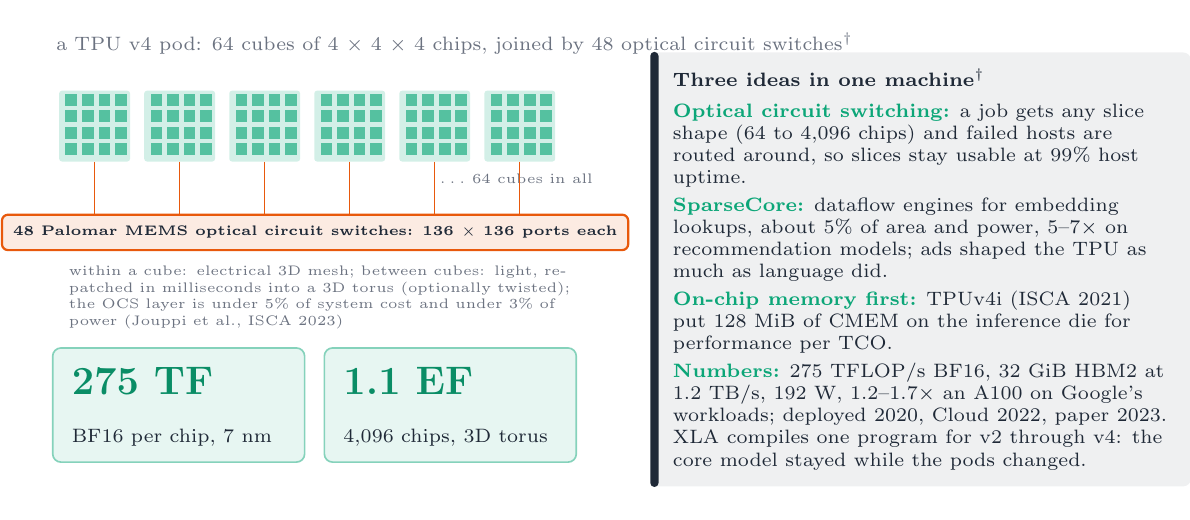
\begin{tikzpicture}
  \useasboundingbox (0,0) rectangle (14.4,5.9);
  % cubes and OCS
  \node[lab,anchor=south west] at (0.3,5.5) {a TPU v4 pod: 64 cubes of 4 $\times$ 4 $\times$ 4 chips, joined by 48 optical circuit switches$^\dagger$};
  \begin{scope}[shift={(0.4,2.75)}]
    \foreach \i in {0,...,5}{
      \begin{scope}[shift={(\i*1.08,1.45)}]
        \fill[emb!18,rounded corners=1pt] (0,0) rectangle (0.9,0.9);
        \foreach \c in {0,...,3}{\foreach \r in {0,...,3}{\fill[emb!70] (0.08+\c*0.21,0.08+\r*0.21) rectangle ++(0.15,0.15);}}
      \end{scope}}
    \node[font=\tiny,text=muted,anchor=north east] at (6.9,1.42) {$\ldots$ 64 cubes in all};
    \node[comp=attn,minimum width=6.4cm,minimum height=0.45cm,font=\fontsize{5.2}{6}\selectfont\bfseries,text=ink] (ocs) at (3.25,0.55) {48 Palomar MEMS optical circuit switches: 136 $\times$ 136 ports each};
    \foreach \i in {0,...,5}{\draw[attn,line width=0.5pt] (\i*1.08+0.45,1.45) -- (\i*1.08+0.45,0.78);}
    \node[font=\tiny,text=muted,anchor=north west,text width=6.7cm] at (0,0.25) {within a cube: electrical 3D mesh; between cubes: light, re-patched in milliseconds into a 3D torus (optionally twisted); the OCS layer is under 5\% of system cost and under 3\% of power (Jouppi et al., ISCA 2023)};
  \end{scope}
  \stat{0.3}{1.85}{275 TF}{BF16 per chip, 7 nm}{emb}
  \stat{3.75}{1.85}{1.1 EF}{4{,}096 chips, 3D torus}{emb}
  \bgpanels{7.9}{5.6}{6.3cm}{Three ideas in one machine$^\dagger$}{%
    \hl{emb}{Optical circuit switching:} a job gets any slice shape
    (64 to 4{,}096 chips) and failed hosts are routed around,
    so slices stay usable at 99\% host uptime.\\[2pt]
    \hl{emb}{SparseCore:} dataflow engines for embedding lookups,
    about 5\% of area and power, 5--7$\times$ on recommendation
    models; ads shaped the TPU as much as language did.\\[2pt]
    \hl{emb}{On-chip memory first:} TPUv4i (ISCA 2021) put 128 MiB
    of CMEM on the inference die for performance per TCO.\\[2pt]
    \hl{emb}{Numbers:} 275 TFLOP/s BF16, 32 GiB HBM2 at 1.2 TB/s,
    192 W, 1.2--1.7$\times$ an A100 on Google's workloads; deployed
    2020, Cloud 2022, paper 2023. XLA compiles one program for v2
    through v4: the core model stayed while the pods changed.}
\end{tikzpicture}
\end{frame}

% ---------------------------------------------------------------- 11
\begin{frame}{v5e to TPU 8: an inference line, a training line, FP8 and FP4}
\framesubtitle{Trillium quadrupled v5e; Ironwood added FP8 and 9,216-chip pods; generation 8 splits training from inference.}
\centering
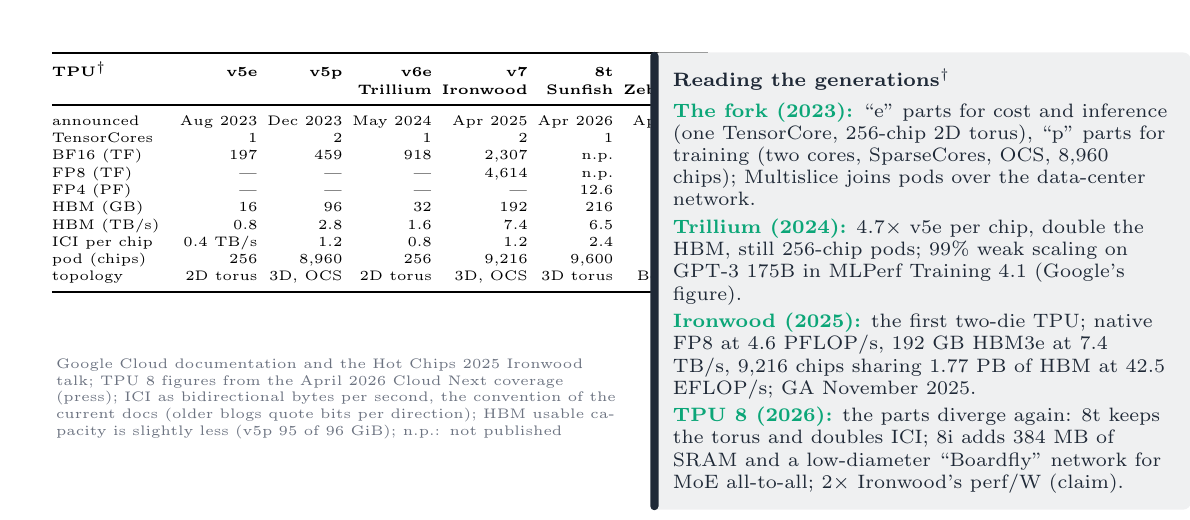
\begin{tikzpicture}
  \useasboundingbox (0,0) rectangle (14.4,5.9);
  \node[anchor=north west,inner sep=0,font=\fontsize{5.0}{6.0}\selectfont] at (0.3,5.6) {%
    \renewcommand{\arraystretch}{1.04}\setlength{\tabcolsep}{1.8pt}%
    \begin{tabular}{@{}>{\raggedright\arraybackslash}p{1.5cm}rrrrrr@{}}
      \toprule
      \textbf{TPU}$^\dagger$ & \textbf{v5e} & \textbf{v5p} & \textbf{v6e} & \textbf{v7} & \textbf{8t} & \textbf{8i}\\
       & & & \textbf{Trillium} & \textbf{Ironwood} & \textbf{Sunfish} & \textbf{Zebrafish}\\
      \midrule
      announced & Aug 2023 & Dec 2023 & May 2024 & Apr 2025 & Apr 2026 & Apr 2026\\
      TensorCores & 1 & 2 & 1 & 2 & 1 & 2\\
      BF16 (TF) & 197 & 459 & 918 & 2{,}307 & n.p. & n.p.\\
      FP8 (TF) & --- & --- & --- & 4{,}614 & n.p. & n.p.\\
      FP4 (PF) & --- & --- & --- & --- & 12.6 & 10.1\\
      HBM (GB) & 16 & 96 & 32 & 192 & 216 & 288\\
      HBM (TB/s) & 0.8 & 2.8 & 1.6 & 7.4 & 6.5 & 8.6\\
      ICI per chip & 0.4 TB/s & 1.2 & 0.8 & 1.2 & 2.4 & n.p.\\
      pod (chips) & 256 & 8{,}960 & 256 & 9{,}216 & 9{,}600 & n.p.\\
      topology & 2D torus & 3D, OCS & 2D torus & 3D, OCS & 3D torus & Boardfly\\
      \bottomrule
    \end{tabular}};
  \node[lab,font=\tiny,anchor=north west,text width=7.2cm] at (0.3,1.75) {Google Cloud documentation and the Hot Chips 2025 Ironwood talk; TPU 8 figures from the April 2026 Cloud Next coverage (press); ICI as bidirectional bytes per second, the convention of the current docs (older blogs quote bits per direction); HBM usable capacity is slightly less (v5p 95 of 96 GiB); n.p.: not published};
  \bgpanels{7.9}{5.6}{6.3cm}{Reading the generations$^\dagger$}{%
    \hl{emb}{The fork (2023):} ``e'' parts for cost and inference
    (one TensorCore, 256-chip 2D torus), ``p'' parts for training
    (two cores, SparseCores, OCS, 8{,}960 chips); Multislice joins
    pods over the data-center network.\\[2pt]
    \hl{emb}{Trillium (2024):} 4.7$\times$ v5e per chip, double the
    HBM, still 256-chip pods; 99\% weak scaling on GPT-3 175B in
    MLPerf Training 4.1 (Google's figure).\\[2pt]
    \hl{emb}{Ironwood (2025):} the first two-die TPU; native FP8 at
    4.6 PFLOP/s, 192 GB HBM3e at 7.4 TB/s, 9{,}216 chips sharing 1.77
    PB of HBM at 42.5 EFLOP/s; GA November 2025.\\[2pt]
    \hl{emb}{TPU 8 (2026):} the parts diverge again: 8t keeps the
    torus and doubles ICI; 8i adds 384 MB of SRAM and a low-diameter
    ``Boardfly'' network for MoE all-to-all; 2$\times$ Ironwood's
    perf/W (claim).}
\end{tikzpicture}
\end{frame}

% ---------------------------------------------------------------- 12
\begin{frame}{The TPU as a business: Google's own, then everyone's}
\framesubtitle{For eight years the TPU was Google's own; in 2025--26 it became the first ASIC sold to others at gigawatt scale.}
\centering
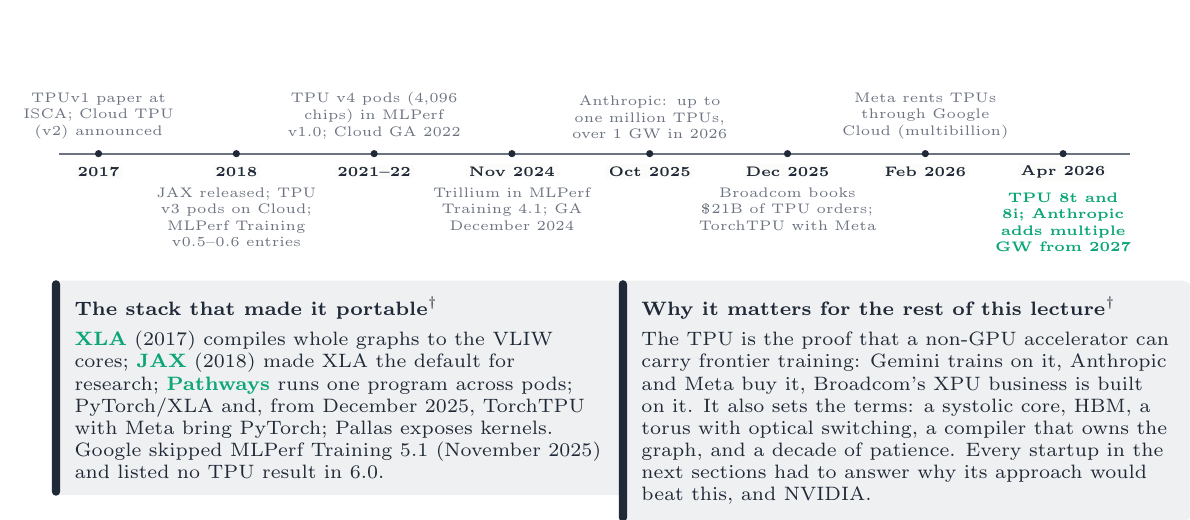
\begin{tikzpicture}
  \useasboundingbox (0,0) rectangle (14.4,5.9);
  \draw[muted,line width=0.8pt] (0.4,4.3) -- (14.0,4.3);
  \foreach \x in {0.9,2.65,4.4,6.15,7.9,9.65,11.4,13.15}{\fill[ink] (\x,4.3) circle (1.3pt);}
  \foreach \yr/\x in {2017/0.9,2018/2.65,2021--22/4.4,Nov 2024/6.15,Oct 2025/7.9,Dec 2025/9.65,Feb 2026/11.4,Apr 2026/13.15}{\node[font=\tiny\bfseries,text=ink,fill=paper,inner sep=1pt] at (\x,4.07) {\yr};}
  \node[lab,anchor=south,text width=2.4cm,align=center,font=\tiny] at (0.9,4.43) {TPUv1 paper at ISCA; Cloud TPU (v2) announced};
  \node[lab,anchor=north,text width=2.4cm,align=center,font=\tiny] at (2.65,3.93) {JAX released; TPU v3 pods on Cloud; MLPerf Training v0.5--0.6 entries};
  \node[lab,anchor=south,text width=2.4cm,align=center,font=\tiny] at (4.4,4.43) {TPU v4 pods (4{,}096 chips) in MLPerf v1.0; Cloud GA 2022};
  \node[lab,anchor=north,text width=2.4cm,align=center,font=\tiny] at (6.15,3.93) {Trillium in MLPerf Training 4.1; GA December 2024};
  \node[lab,anchor=south,text width=2.4cm,align=center,font=\tiny] at (7.9,4.43) {Anthropic: up to one million TPUs, over 1 GW in 2026};
  \node[lab,anchor=north,text width=2.4cm,align=center,font=\tiny] at (9.65,3.93) {Broadcom books \$21B of TPU orders; TorchTPU with Meta};
  \node[lab,anchor=south,text width=2.4cm,align=center,font=\tiny] at (11.4,4.43) {Meta rents TPUs through Google Cloud (multibillion)};
  \node[anchor=north,text width=2.4cm,align=center,font=\tiny\bfseries,text=emb] at (13.15,3.93) {TPU 8t and 8i; Anthropic adds multiple GW from 2027};
  \bgpanels{0.3}{2.7}{6.7cm}{The stack that made it portable$^\dagger$}{%
    \hl{emb}{XLA} (2017) compiles whole graphs to the VLIW cores;
    \hl{emb}{JAX} (2018) made XLA the default for research;
    \hl{emb}{Pathways} runs one program across pods; PyTorch/XLA and,
    from December 2025, TorchTPU with Meta bring PyTorch; Pallas
    exposes kernels. Google skipped MLPerf Training 5.1 (November
    2025) and listed no TPU result in 6.0.}
  \bgpanels{7.5}{2.7}{6.7cm}{Why it matters for the rest of this lecture$^\dagger$}{%
    The TPU is the proof that a non-GPU accelerator can carry
    frontier training: Gemini trains on it, Anthropic and Meta buy
    it, Broadcom's XPU business is built on it. It also sets the
    terms: a systolic core, HBM, a torus with optical switching, a
    compiler that owns the graph, and a decade of patience. Every
    startup in the next sections had to answer why its approach
    would beat this, and NVIDIA.}
\end{tikzpicture}
\end{frame}

% ---------------------------------------------------------------- 13
\stage{4}
\begin{frame}{Cerebras: the wafer is the chip}
\framesubtitle{84 reticle fields wired across the scribe lines, spare cores for yield, 44 GB of SRAM on one 46,225 mm$^2$ die.}
\centering
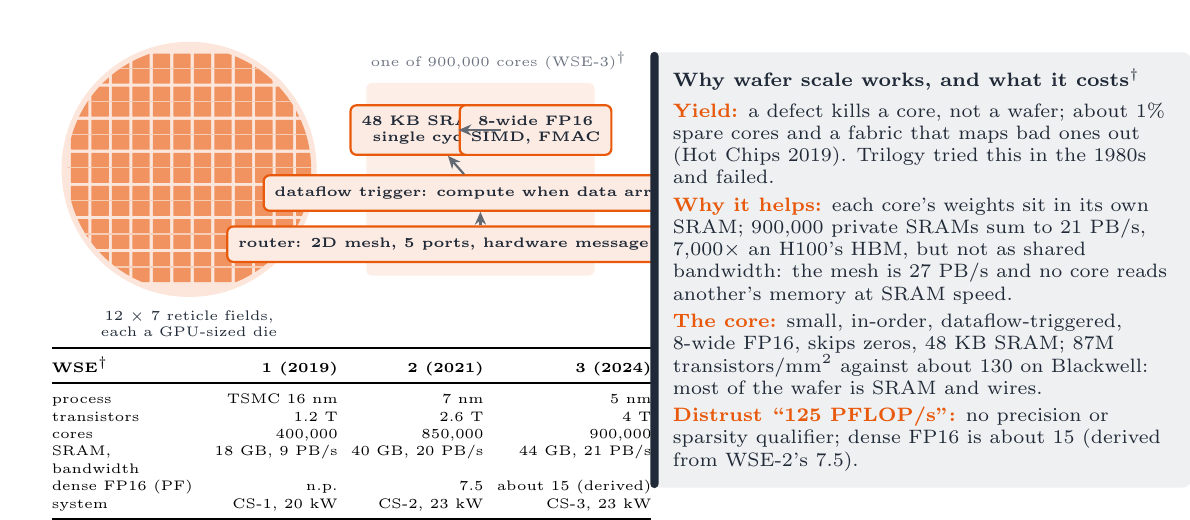
\begin{tikzpicture}
  \useasboundingbox (0,0) rectangle (14.4,5.9);
  % wafer with reticle fields
  \begin{scope}[shift={(0.5,2.55)}]
    \fill[attn!15] (1.55,1.55) circle (1.62);
    \begin{scope}
      \clip (1.55,1.55) circle (1.55);
      \foreach \c in {0,...,11}{\foreach \r in {0,...,6}{\fill[attn!65,rounded corners=0.2pt] (0.05+\c*0.26,0.12+\r*0.42) rectangle ++(0.22,0.38);}}
      \foreach \r in {0,...,6}{\draw[attn!30!white,line width=0.4pt] (0,0.31+\r*0.42) -- (3.2,0.31+\r*0.42);}
    \end{scope}
    \node[font=\tiny,text=ink,anchor=north,text width=3.4cm,align=center] at (1.55,-0.12) {12 $\times$ 7 reticle fields, each a GPU-sized die};
  \end{scope}
  % one core
  \begin{scope}[shift={(4.3,2.75)}]
    \node[lab,anchor=south west,font=\tiny] at (0,2.55) {one of 900,000 cores (WSE-3)$^\dagger$};
    \fill[attn!10,rounded corners=2pt] (0,0) rectangle (2.9,2.45);
    \node[comp=attn,minimum width=1.2cm,minimum height=0.5cm,font=\fontsize{4.6}{5.5}\selectfont\bfseries,text=ink,align=center] (sram) at (0.75,1.85) {48 KB SRAM\\single cycle};
    \node[comp=attn,minimum width=1.2cm,minimum height=0.5cm,font=\fontsize{4.6}{5.5}\selectfont\bfseries,text=ink,align=center] (simd) at (2.15,1.85) {8-wide FP16\\SIMD, FMAC};
    \node[comp=attn,minimum width=2.6cm,minimum height=0.45cm,font=\fontsize{4.6}{5.5}\selectfont\bfseries,text=ink,align=center] (sched) at (1.45,1.05) {dataflow trigger: compute when data arrives};
    \node[comp=attn,minimum width=2.6cm,minimum height=0.45cm,font=\fontsize{4.6}{5.5}\selectfont\bfseries,text=ink,align=center] (rtr) at (1.45,0.4) {router: 2D mesh, 5 ports, hardware message passing};
    \draw[flow] (sram) -- (simd); \draw[flow] (sched) -- (sram); \draw[flow] (rtr) -- (sched);
  \end{scope}
  \node[anchor=north west,inner sep=0,font=\fontsize{5.4}{6.3}\selectfont] at (0.3,1.85) {%
    \renewcommand{\arraystretch}{1.0}\setlength{\tabcolsep}{2.4pt}%
    \begin{tabular}{@{}>{\raggedright\arraybackslash}p{1.9cm}rrr@{}}
      \toprule
      \textbf{WSE}$^\dagger$ & \textbf{1 (2019)} & \textbf{2 (2021)} & \textbf{3 (2024)}\\
      \midrule
      process & TSMC 16 nm & 7 nm & 5 nm\\
      transistors & 1.2 T & 2.6 T & 4 T\\
      cores & 400{,}000 & 850{,}000 & 900{,}000\\
      SRAM, bandwidth & 18 GB, 9 PB/s & 40 GB, 20 PB/s & 44 GB, 21 PB/s\\
      dense FP16 (PF) & n.p. & 7.5 & about 15 (derived)\\
      system & CS-1, 20 kW & CS-2, 23 kW & CS-3, 23 kW\\
      \bottomrule
    \end{tabular}};
  \bgpanels{7.9}{5.6}{6.3cm}{Why wafer scale works, and what it costs$^\dagger$}{%
    \hl{attn}{Yield:} a defect kills a core, not a wafer; about 1\%
    spare cores and a fabric that maps bad ones out (Hot Chips
    2019). Trilogy tried this in the 1980s and failed.\\[2pt]
    \hl{attn}{Why it helps:} each core's weights sit in its own SRAM;
    900{,}000 private SRAMs sum to 21 PB/s, 7{,}000$\times$ an H100's
    HBM, but not as shared bandwidth: the mesh is 27 PB/s and no core
    reads another's memory at SRAM speed.\\[2pt]
    \hl{attn}{The core:} small, in-order, dataflow-triggered, 8-wide
    FP16, skips zeros, 48 KB SRAM; 87M transistors/mm$^2$ against
    about 130 on Blackwell: most of the wafer is SRAM and wires.\\[2pt]
    \hl{attn}{Distrust ``125 PFLOP/s'':} no precision or sparsity
    qualifier; dense FP16 is about 15 (derived from WSE-2's 7.5).}
\end{tikzpicture}
\end{frame}

% ---------------------------------------------------------------- 14
\begin{frame}{Weight streaming: MemoryX, SwarmX and Condor Galaxy}
\framesubtitle{Activations stay on the wafer, weights stream in layer by layer from outside; clusters scale by data parallelism.}
\centering
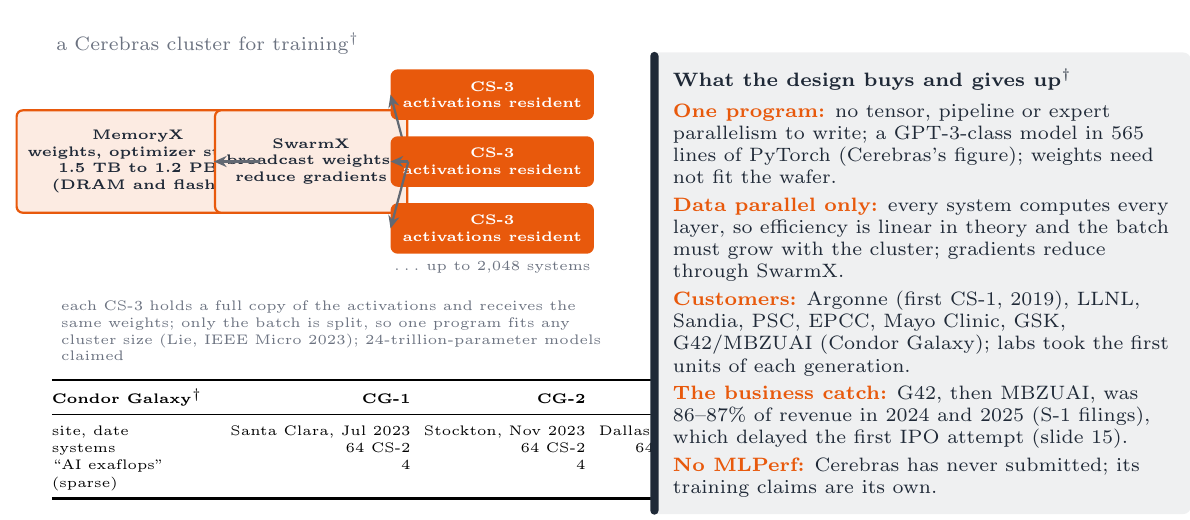
\begin{tikzpicture}
  \useasboundingbox (0,0) rectangle (14.4,5.9);
  \node[lab,anchor=south west] at (0.3,5.5) {a Cerebras cluster for training$^\dagger$};
  \begin{scope}[shift={(0.3,2.6)}]
    \node[comp=attn,minimum width=2.1cm,minimum height=1.3cm,font=\fontsize{5}{6}\selectfont\bfseries,text=ink,align=center] (mx) at (1.1,1.6) {MemoryX\\weights, optimizer state\\1.5 TB to 1.2 PB\\(DRAM and flash)};
    \node[comp=attn,minimum width=1.5cm,minimum height=1.3cm,font=\fontsize{5}{6}\selectfont\bfseries,text=ink,align=center] (sw) at (3.3,1.6) {SwarmX\\broadcast weights,\\reduce gradients};
    \foreach \i/\y in {0/2.45,1/1.6,2/0.75}{\node[comp=attn,minimum width=1.5cm,minimum height=0.6cm,font=\fontsize{5}{6}\selectfont\bfseries,text=white,fill=attn,align=center] (cs\i) at (5.6,\y) {CS-3\\activations resident};
      \draw[flow] (sw.east) -- (cs\i.west);}
    \node[font=\tiny,text=muted] at (5.6,0.25) {$\ldots$ up to 2{,}048 systems};
    \draw[flow] (mx) -- (sw);
    \node[font=\tiny,text=muted,anchor=north west,text width=6.9cm] at (0,-0.05) {each CS-3 holds a full copy of the activations and receives the same weights; only the batch is split, so one program fits any cluster size (Lie, IEEE Micro 2023); 24-trillion-parameter models claimed};
  \end{scope}
  \node[anchor=north west,inner sep=0,font=\fontsize{5.4}{6.3}\selectfont] at (0.3,1.45) {%
    \renewcommand{\arraystretch}{1.0}\setlength{\tabcolsep}{2.4pt}%
    \begin{tabular}{@{}>{\raggedright\arraybackslash}p{2.1cm}rrr@{}}
      \toprule
      \textbf{Condor Galaxy}$^\dagger$ & \textbf{CG-1} & \textbf{CG-2} & \textbf{CG-3}\\
      \midrule
      site, date & Santa Clara, Jul 2023 & Stockton, Nov 2023 & Dallas, 2024\\
      systems & 64 CS-2 & 64 CS-2 & 64 CS-3\\
      ``AI exaflops'' (sparse) & 4 & 4 & 8\\
      \bottomrule
    \end{tabular}};
  \bgpanels{7.9}{5.6}{6.3cm}{What the design buys and gives up$^\dagger$}{%
    \hl{attn}{One program:} no tensor, pipeline or expert
    parallelism to write; a GPT-3-class model in 565 lines of
    PyTorch (Cerebras's figure); weights need not fit the wafer.\\[2pt]
    \hl{attn}{Data parallel only:} every system computes every
    layer, so efficiency is linear in theory and the batch must
    grow with the cluster; gradients reduce through SwarmX.\\[2pt]
    \hl{attn}{Customers:} Argonne (first CS-1, 2019), LLNL, Sandia,
    PSC, EPCC, Mayo Clinic, GSK, G42/MBZUAI (Condor Galaxy); labs
    took the first units of each generation.\\[2pt]
    \hl{attn}{The business catch:} G42, then MBZUAI, was 86--87\% of
    revenue in 2024 and 2025 (S-1 filings), which delayed the first
    IPO attempt (slide 15).\\[2pt]
    \hl{attn}{No MLPerf:} Cerebras has never submitted; its training
    claims are its own.}
\end{tikzpicture}
\end{frame}

% ---------------------------------------------------------------- 15
\begin{frame}{Cerebras Inference, the CS-4, and the IPO}
\framesubtitle{From August 2024 the wafer became an inference engine; speed per user, not training, took it public.}
\centering
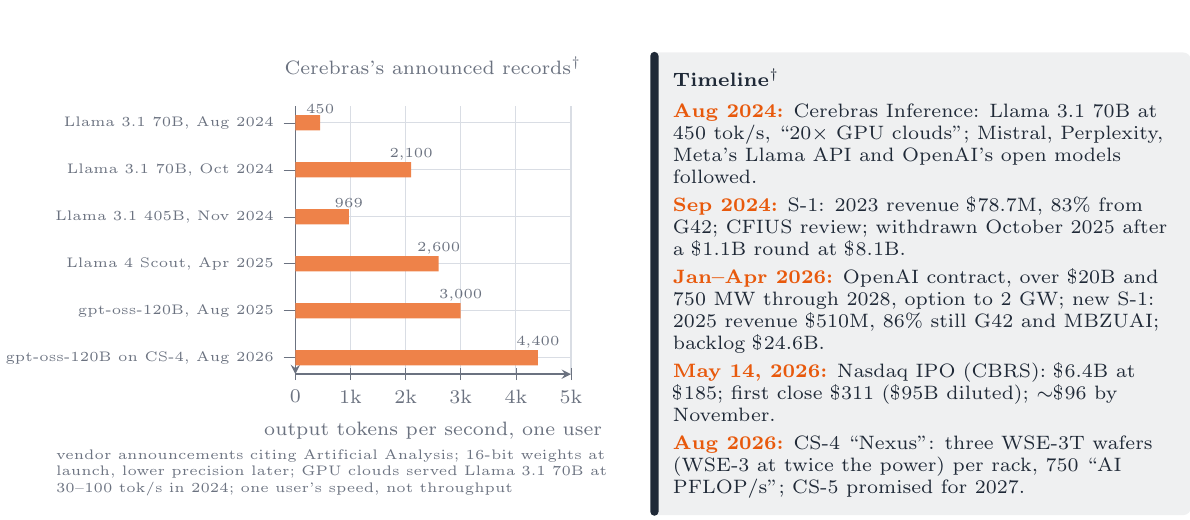
\begin{tikzpicture}
  \useasboundingbox (0,0) rectangle (14.4,5.9);
  \begin{scope}[shift={(3.4,1.5)}]
  \begin{axis}[lecture,scale only axis,width=3.5cm,height=3.4cm,xbar,bar width=5.5pt,xmin=0,xmax=5000,enlarge y limits=0.07,
      symbolic y coords={{Llama 3.1 70B, Aug 2024},{Llama 3.1 70B, Oct 2024},{Llama 3.1 405B, Nov 2024},{Llama 4 Scout, Apr 2025},{gpt-oss-120B, Aug 2025},{gpt-oss-120B on CS-4, Aug 2026}},
      ytick=data,y dir=reverse,yticklabel style={font=\tiny},xlabel={output tokens per second, one user},
      xtick={0,1000,2000,3000,4000,5000},xticklabels={0,1k,2k,3k,4k,5k},
      nodes near coords,nodes near coords style={font=\tiny,text=muted},point meta=explicit symbolic,
      title style={font=\scriptsize,text=muted,at={(0.5,1.02)}},title={Cerebras's announced records$^\dagger$}]
    \addplot[fill=attn!75,draw=none] coordinates {(450,{Llama 3.1 70B, Aug 2024})[450] (2100,{Llama 3.1 70B, Oct 2024})[2{,}100] (969,{Llama 3.1 405B, Nov 2024})[969] (2600,{Llama 4 Scout, Apr 2025})[2{,}600] (3000,{gpt-oss-120B, Aug 2025})[3{,}000] (4400,{gpt-oss-120B on CS-4, Aug 2026})[4{,}400]};
  \end{axis}
  \end{scope}
  \node[lab,font=\tiny,anchor=north west,text width=7.2cm] at (0.3,0.6) {vendor announcements citing Artificial Analysis; 16-bit weights at launch, lower precision later; GPU clouds served Llama 3.1 70B at 30--100 tok/s in 2024; one user's speed, not throughput};
  \bgpanels{7.9}{5.6}{6.3cm}{Timeline$^\dagger$}{%
    \hl{attn}{Aug 2024:} Cerebras Inference: Llama 3.1 70B at 450
    tok/s, ``20$\times$ GPU clouds''; Mistral, Perplexity, Meta's
    Llama API and OpenAI's open models followed.\\[2pt]
    \hl{attn}{Sep 2024:} S-1: 2023 revenue \$78.7M, 83\% from G42;
    CFIUS review; withdrawn October 2025 after a \$1.1B round at
    \$8.1B.\\[2pt]
    \hl{attn}{Jan--Apr 2026:} OpenAI contract, over \$20B and 750 MW
    through 2028, option to 2 GW; new S-1: 2025 revenue \$510M, 86\%
    still G42 and MBZUAI; backlog \$24.6B.\\[2pt]
    \hl{attn}{May 14, 2026:} Nasdaq IPO (CBRS): \$6.4B at \$185;
    first close \$311 (\$95B diluted); ${\sim}$\$96 by November.\\[2pt]
    \hl{attn}{Aug 2026:} CS-4 ``Nexus'': three WSE-3T wafers (WSE-3
    at twice the power) per rack, 750 ``AI PFLOP/s''; CS-5 promised
    for 2027.}
\end{tikzpicture}
\end{frame}

% ---------------------------------------------------------------- 16
\stage{5}
\begin{frame}{Groq: a deterministic tensor streaming processor}
\framesubtitle{One core, 220 MiB of SRAM, no DRAM, every cycle scheduled by the compiler; Llama 2 70B took 576 chips.}
\centering
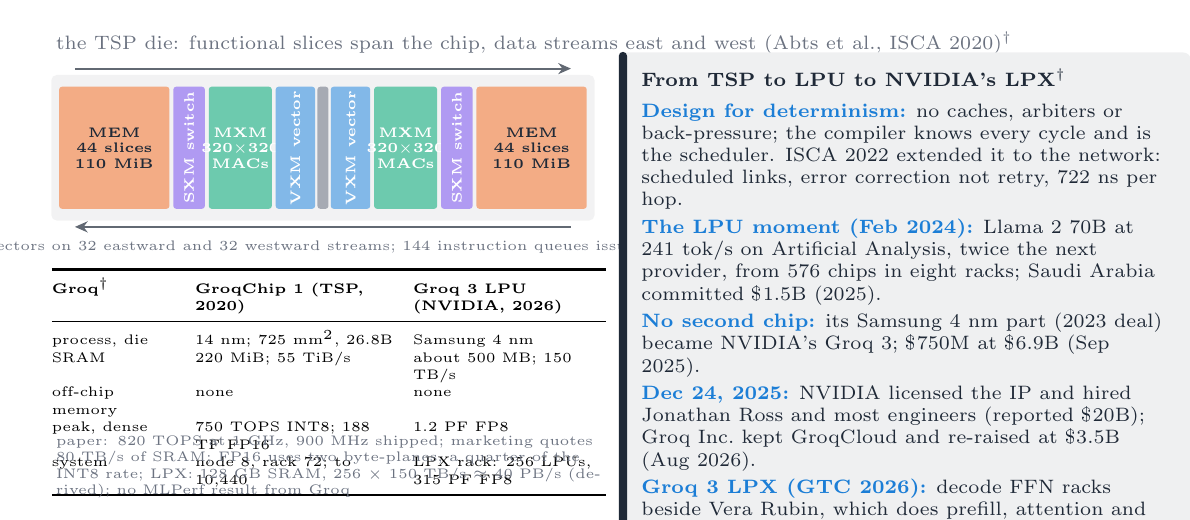
\begin{tikzpicture}
  \useasboundingbox (0,0) rectangle (14.4,5.9);
  \node[lab,anchor=south west] at (0.3,5.5) {the TSP die: functional slices span the chip, data streams east and west (Abts et al., ISCA 2020)$^\dagger$};
  \begin{scope}[shift={(0.3,3.45)}]
    \fill[ink!6,rounded corners=2pt] (0,0) rectangle (6.9,1.85);
    \fill[attn!50,rounded corners=1pt] (0.1,0.15) rectangle (1.5,1.7);
    \node[font=\fontsize{4.6}{5.5}\selectfont\bfseries,text=ink,align=center] at (0.8,0.92) {MEM\\44 slices\\110 MiB};
    \fill[posc!55,rounded corners=1pt] (1.55,0.15) rectangle (1.95,1.7);
    \node[font=\fontsize{4.4}{5}\selectfont\bfseries,text=white,rotate=90] at (1.75,0.92) {SXM switch};
    \fill[emb!60,rounded corners=1pt] (2.0,0.15) rectangle (2.8,1.7);
    \node[font=\fontsize{4.6}{5.5}\selectfont\bfseries,text=white,align=center] at (2.4,0.92) {MXM\\320$\times$320\\MACs};
    \fill[mlp!55,rounded corners=1pt] (2.85,0.15) rectangle (3.35,1.7);
    \node[font=\fontsize{4.4}{5}\selectfont\bfseries,text=white,rotate=90] at (3.1,0.92) {VXM vector};
    \fill[muted!60,rounded corners=1pt] (3.38,0.15) rectangle (3.52,1.7);
    \fill[mlp!55,rounded corners=1pt] (3.55,0.15) rectangle (4.05,1.7);
    \node[font=\fontsize{4.4}{5}\selectfont\bfseries,text=white,rotate=90] at (3.8,0.92) {VXM vector};
    \fill[emb!60,rounded corners=1pt] (4.1,0.15) rectangle (4.9,1.7);
    \node[font=\fontsize{4.6}{5.5}\selectfont\bfseries,text=white,align=center] at (4.5,0.92) {MXM\\320$\times$320\\MACs};
    \fill[posc!55,rounded corners=1pt] (4.95,0.15) rectangle (5.35,1.7);
    \node[font=\fontsize{4.4}{5}\selectfont\bfseries,text=white,rotate=90] at (5.15,0.92) {SXM switch};
    \fill[attn!50,rounded corners=1pt] (5.4,0.15) rectangle (6.8,1.7);
    \node[font=\fontsize{4.6}{5.5}\selectfont\bfseries,text=ink,align=center] at (6.1,0.92) {MEM\\44 slices\\110 MiB};
    \draw[flow,ink!70] (0.3,1.93) -- (6.6,1.93);
    \draw[flow,ink!70] (6.6,-0.08) -- (0.3,-0.08);
    \node[font=\fontsize{4.4}{5}\selectfont,text=muted,anchor=north] at (3.45,-0.14) {320-wide vectors on 32 eastward and 32 westward streams; 144 instruction queues issue in lock step};
  \end{scope}
  \node[anchor=north west,inner sep=0,font=\fontsize{5.4}{6.3}\selectfont] at (0.3,2.85) {%
    \renewcommand{\arraystretch}{1.0}\setlength{\tabcolsep}{2.4pt}%
    \begin{tabular}{@{}>{\raggedright\arraybackslash}p{1.65cm}>{\raggedright\arraybackslash}p{2.6cm}>{\raggedright\arraybackslash}p{2.45cm}@{}}
      \toprule
      \textbf{Groq}$^\dagger$ & \textbf{GroqChip 1 (TSP, 2020)} & \textbf{Groq 3 LPU (NVIDIA, 2026)}\\
      \midrule
      process, die & 14 nm; 725 mm$^2$, 26.8B & Samsung 4 nm\\
      SRAM & 220 MiB; 55 TiB/s & about 500 MB; 150 TB/s\\
      off-chip memory & none & none\\
      peak, dense & 750 TOPS INT8; 188 TF FP16 & 1.2 PF FP8\\
      system & node 8, rack 72; to 10{,}440 & LPX rack: 256 LPUs, 315 PF FP8\\
      \bottomrule
    \end{tabular}};
  \node[lab,font=\tiny,anchor=north west,text width=7.0cm] at (0.3,0.78) {paper: 820 TOPS at 1 GHz, 900 MHz shipped; marketing quotes 80 TB/s of SRAM; FP16 uses two byte-planes, a quarter of the INT8 rate; LPX: 128 GB SRAM, 256 $\times$ 150 TB/s $\approx$ 40 PB/s (derived); no MLPerf result from Groq};
  \bgpanels{7.5}{5.6}{6.7cm}{From TSP to LPU to NVIDIA's LPX$^\dagger$}{%
    \hl{mlp}{Design for determinism:} no caches, arbiters or
    back-pressure; the compiler knows every cycle and is the
    scheduler. ISCA 2022 extended it to the network: scheduled
    links, error correction not retry, 722 ns per hop.\\[2pt]
    \hl{mlp}{The LPU moment (Feb 2024):} Llama 2 70B at 241 tok/s on
    Artificial Analysis, twice the next provider, from 576 chips in
    eight racks; Saudi Arabia committed \$1.5B (2025).\\[2pt]
    \hl{mlp}{No second chip:} its Samsung 4 nm part (2023 deal)
    became NVIDIA's Groq 3; \$750M at \$6.9B (Sep 2025).\\[2pt]
    \hl{mlp}{Dec 24, 2025:} NVIDIA licensed the IP and hired Jonathan
    Ross and most engineers (reported \$20B); Groq Inc.\ kept
    GroqCloud and re-raised at \$3.5B (Aug 2026).\\[2pt]
    \hl{mlp}{Groq 3 LPX (GTC 2026):} decode FFN racks beside Vera
    Rubin, which does prefill, attention and KV; Gemma 4 31B at
    3{,}431 tok/s (private endpoint); ships late 2026.}
\end{tikzpicture}
\end{frame}

% ---------------------------------------------------------------- 17
\begin{frame}{SambaNova: reconfigurable dataflow, three memory tiers}
\framesubtitle{Compute and memory units wired per model by the compiler; SRAM, HBM and DDR hold a trillion parameters.}
\centering
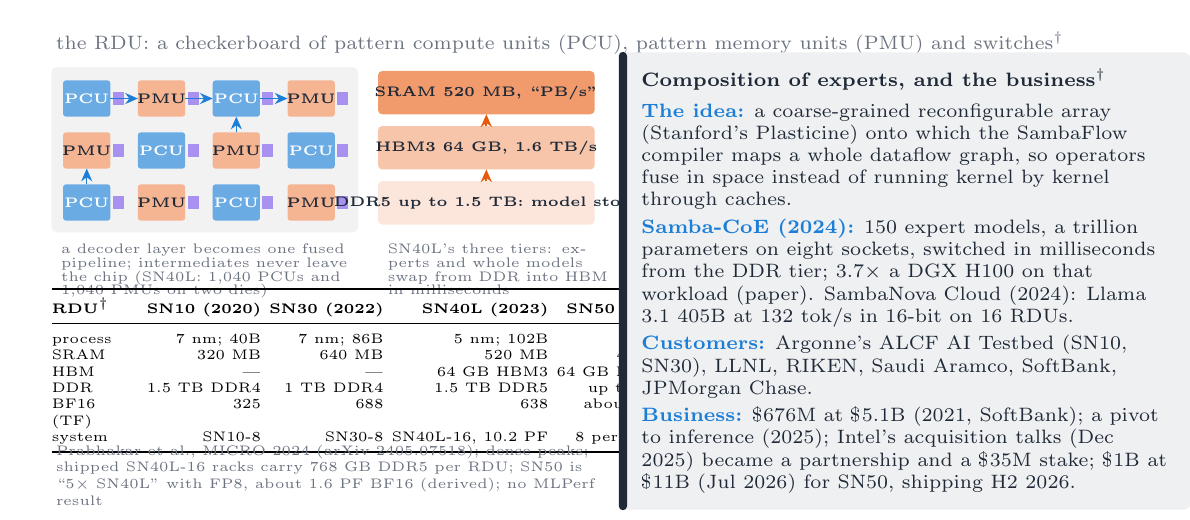
\begin{tikzpicture}
  \useasboundingbox (0,0) rectangle (14.4,5.9);
  \node[lab,anchor=south west] at (0.3,5.5) {the RDU: a checkerboard of pattern compute units (PCU), pattern memory units (PMU) and switches$^\dagger$};
  \begin{scope}[shift={(0.3,3.3)}]
    \fill[ink!6,rounded corners=2pt] (0,0) rectangle (3.9,2.1);
    \foreach \r in {0,1,2}{\foreach \c in {0,1,2,3}{
      \pgfmathparse{int(mod(\r+\c,2))}
      \ifnum\pgfmathresult=0
        \fill[mlp!65,rounded corners=1pt] (0.15+\c*0.95,0.15+\r*0.66) rectangle ++(0.6,0.46);
        \node[font=\fontsize{4.2}{5}\selectfont\bfseries,text=white] at (0.45+\c*0.95,0.38+\r*0.66) {PCU};
      \else
        \fill[attn!45,rounded corners=1pt] (0.15+\c*0.95,0.15+\r*0.66) rectangle ++(0.6,0.46);
        \node[font=\fontsize{4.2}{5}\selectfont\bfseries,text=ink] at (0.45+\c*0.95,0.38+\r*0.66) {PMU};
      \fi
      \fill[posc!60] (0.78+\c*0.95,0.3+\r*0.66) rectangle ++(0.14,0.16);}}
    \draw[thinflow,mlp] (0.75,1.7) -- (1.1,1.7); \draw[thinflow,mlp] (1.7,1.7) -- (2.05,1.7); \draw[thinflow,mlp] (2.65,1.7) -- (3.0,1.7);
    \draw[thinflow,mlp] (0.45,0.61) -- (0.45,0.81); \draw[thinflow,mlp] (2.35,1.27) -- (2.35,1.47);
    \node[font=\fontsize{4.4}{5}\selectfont,text=muted,anchor=north west,text width=3.9cm] at (0,-0.02) {a decoder layer becomes one fused pipeline; intermediates never leave the chip (SN40L: 1{,}040 PCUs and 1{,}040 PMUs on two dies)};
  \end{scope}
  \begin{scope}[shift={(4.45,3.3)}]
    \fill[attn!60,rounded corners=1.5pt] (0,1.5) rectangle (2.75,2.05);
    \node[font=\fontsize{4.6}{5.5}\selectfont\bfseries,text=ink] at (1.375,1.775) {SRAM 520 MB, ``PB/s''};
    \fill[attn!35,rounded corners=1.5pt] (0,0.8) rectangle (2.75,1.35);
    \node[font=\fontsize{4.6}{5.5}\selectfont\bfseries,text=ink] at (1.375,1.075) {HBM3 64 GB, 1.6 TB/s};
    \fill[attn!15,rounded corners=1.5pt] (0,0.1) rectangle (2.75,0.65);
    \node[font=\fontsize{4.6}{5.5}\selectfont\bfseries,text=ink] at (1.375,0.375) {DDR5 up to 1.5 TB: model store};
    \draw[flow,attn] (1.375,0.65) -- (1.375,0.8); \draw[flow,attn] (1.375,1.35) -- (1.375,1.5);
    \node[font=\fontsize{4.4}{5}\selectfont,text=muted,anchor=north west,text width=2.8cm] at (0,-0.02) {SN40L's three tiers: experts and whole models swap from DDR into HBM in milliseconds};
  \end{scope}
  \node[anchor=north west,inner sep=0,font=\fontsize{5.0}{5.9}\selectfont] at (0.3,2.6) {%
    \renewcommand{\arraystretch}{1.0}\setlength{\tabcolsep}{1.5pt}%
    \begin{tabular}{@{}>{\raggedright\arraybackslash}p{1.1cm}rrrr@{}}
      \toprule
      \textbf{RDU}$^\dagger$ & \textbf{SN10 (2020)} & \textbf{SN30 (2022)} & \textbf{SN40L (2023)} & \textbf{SN50 (2026)}\\
      \midrule
      process & 7 nm; 40B & 7 nm; 86B & 5 nm; 102B & n.p.\\
      SRAM & 320 MB & 640 MB & 520 MB & 432 MB\\
      HBM & --- & --- & 64 GB HBM3 & 64 GB HBM2E\\
      DDR & 1.5 TB DDR4 & 1 TB DDR4 & 1.5 TB DDR5 & up to 2 TB\\
      BF16 (TF) & 325 & 688 & 638 & about 1{,}600\\
      system & SN10-8 & SN30-8 & SN40L-16, 10.2 PF & 8 per chassis\\
      \bottomrule
    \end{tabular}};
  \node[lab,font=\tiny,anchor=north west,text width=7.0cm] at (0.3,0.66) {Prabhakar et al., MICRO 2024 (arXiv 2405.07518); dense peaks; shipped SN40L-16 racks carry 768 GB DDR5 per RDU; SN50 is ``5$\times$ SN40L'' with FP8, about 1.6 PF BF16 (derived); no MLPerf result};
  \bgpanels{7.5}{5.6}{6.7cm}{Composition of experts, and the business$^\dagger$}{%
    \hl{mlp}{The idea:} a coarse-grained reconfigurable array
    (Stanford's Plasticine) onto which the SambaFlow compiler maps a
    whole dataflow graph, so operators fuse in space instead of
    running kernel by kernel through caches.\\[2pt]
    \hl{mlp}{Samba-CoE (2024):} 150 expert models, a trillion
    parameters on eight sockets, switched in milliseconds from the
    DDR tier; 3.7$\times$ a DGX H100 on that workload (paper).
    SambaNova Cloud (2024): Llama 3.1 405B at 132 tok/s in 16-bit on
    16 RDUs.\\[2pt]
    \hl{mlp}{Customers:} Argonne's ALCF AI Testbed (SN10, SN30),
    LLNL, RIKEN, Saudi Aramco, SoftBank, JPMorgan Chase.\\[2pt]
    \hl{mlp}{Business:} \$676M at \$5.1B (2021, SoftBank); a pivot
    to inference (2025); Intel's acquisition talks (Dec 2025) became
    a partnership and a \$35M stake; \$1B at \$11B (Jul 2026) for
    SN50, shipping H2 2026.}
\end{tikzpicture}
\end{frame}

% ---------------------------------------------------------------- 18
\begin{frame}{Graphcore: the IPU and bulk-synchronous parallelism}
\framesubtitle{1,472 MIMD tiles with 900 MB of SRAM exchange data in compiler-scheduled supersteps; sold to SoftBank in 2024.}
\centering
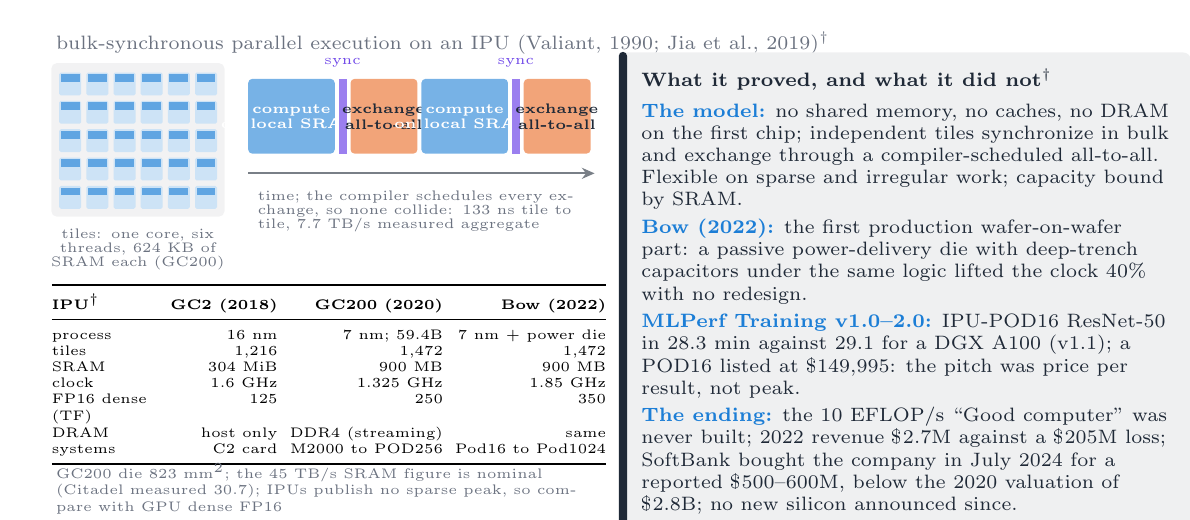
\begin{tikzpicture}
  \useasboundingbox (0,0) rectangle (14.4,5.9);
  \node[lab,anchor=south west] at (0.3,5.5) {bulk-synchronous parallel execution on an IPU (Valiant, 1990; Jia et al., 2019)$^\dagger$};
  \begin{scope}[shift={(0.3,3.5)}]
    \fill[ink!6,rounded corners=2pt] (0,0) rectangle (2.2,1.95);
    \foreach \r in {0,...,4}{\foreach \c in {0,...,5}{\fill[mlp!22,rounded corners=0.6pt] (0.1+\c*0.345,0.1+\r*0.36) rectangle ++(0.28,0.29); \fill[mlp!70] (0.12+\c*0.345,0.27+\r*0.36) rectangle ++(0.24,0.1);}}
    \node[font=\fontsize{4.4}{5}\selectfont,text=muted,anchor=north,text width=2.3cm,align=center] at (1.1,-0.03) {tiles: one core, six threads, 624 KB of SRAM each (GC200)};
    \begin{scope}[shift={(2.5,0.35)}]
      \foreach \i in {0,1}{
        \fill[mlp!60,rounded corners=1.5pt] (\i*2.2,0.45) rectangle ++(1.1,0.95);
        \node[font=\fontsize{4.6}{5.5}\selectfont\bfseries,text=white,align=center] at (\i*2.2+0.55,0.92) {compute\\on local SRAM};
        \fill[posc!70] (\i*2.2+1.15,0.45) rectangle ++(0.1,0.95);
        \node[font=\fontsize{4.2}{5}\selectfont,text=posc,anchor=south] at (\i*2.2+1.2,1.42) {sync};
        \fill[attn!55,rounded corners=1.5pt] (\i*2.2+1.3,0.45) rectangle ++(0.85,0.95);
        \node[font=\fontsize{4.6}{5.5}\selectfont\bfseries,text=ink,align=center] at (\i*2.2+1.72,0.92) {exchange\\all-to-all};}
      \draw[flow,ink!60] (0,0.2) -- (4.4,0.2);
      \node[font=\fontsize{4.4}{5}\selectfont,text=muted,anchor=north west,text width=4.4cm] at (0,0.1) {time; the compiler schedules every exchange, so none collide: 133 ns tile to tile, 7.7 TB/s measured aggregate};
    \end{scope}
  \end{scope}
  \node[anchor=north west,inner sep=0,font=\fontsize{5.3}{6.2}\selectfont] at (0.3,2.65) {%
    \renewcommand{\arraystretch}{0.94}\setlength{\tabcolsep}{2.2pt}%
    \begin{tabular}{@{}>{\raggedright\arraybackslash}p{1.35cm}rrr@{}}
      \toprule
      \textbf{IPU}$^\dagger$ & \textbf{GC2 (2018)} & \textbf{GC200 (2020)} & \textbf{Bow (2022)}\\
      \midrule
      process & 16 nm & 7 nm; 59.4B & 7 nm $+$ power die\\
      tiles & 1{,}216 & 1{,}472 & 1{,}472\\
      SRAM & 304 MiB & 900 MB & 900 MB\\
      clock & 1.6 GHz & 1.325 GHz & 1.85 GHz\\
      FP16 dense (TF) & 125 & 250 & 350\\
      DRAM & host only & DDR4 (streaming) & same\\
      systems & C2 card & M2000 to POD256 & Pod16 to Pod1024\\
      \bottomrule
    \end{tabular}};
  \node[lab,font=\tiny,anchor=north west,text width=7.0cm] at (0.3,0.42) {GC200 die 823 mm$^2$; the 45 TB/s SRAM figure is nominal (Citadel measured 30.7); IPUs publish no sparse peak, so compare with GPU dense FP16};
  \bgpanels{7.5}{5.6}{6.7cm}{What it proved, and what it did not$^\dagger$}{%
    \hl{mlp}{The model:} no shared memory, no caches, no DRAM on the
    first chip; independent tiles synchronize in bulk and exchange
    through a compiler-scheduled all-to-all. Flexible on sparse and
    irregular work; capacity bound by SRAM.\\[2pt]
    \hl{mlp}{Bow (2022):} the first production wafer-on-wafer part:
    a passive power-delivery die with deep-trench capacitors under
    the same logic lifted the clock 40\% with no redesign.\\[2pt]
    \hl{mlp}{MLPerf Training v1.0--2.0:} IPU-POD16 ResNet-50 in 28.3
    min against 29.1 for a DGX A100 (v1.1); a POD16 listed at
    \$149{,}995: the pitch was price per result, not peak.\\[2pt]
    \hl{mlp}{The ending:} the 10 EFLOP/s ``Good computer'' was never
    built; 2022 revenue \$2.7M against a \$205M loss; SoftBank bought
    the company in July 2024 for a reported \$500--600M, below the
    2020 valuation of \$2.8B; no new silicon announced since.}
\end{tikzpicture}
\end{frame}

% ---------------------------------------------------------------- 19
\begin{frame}{Tenstorrent: Tensix cores, RISC-V and an open stack}
\framesubtitle{Clusters of five small RISC-V cores around a matrix engine and 1.5 MB of SRAM, meshed; Ethernet on the die.}
\centering
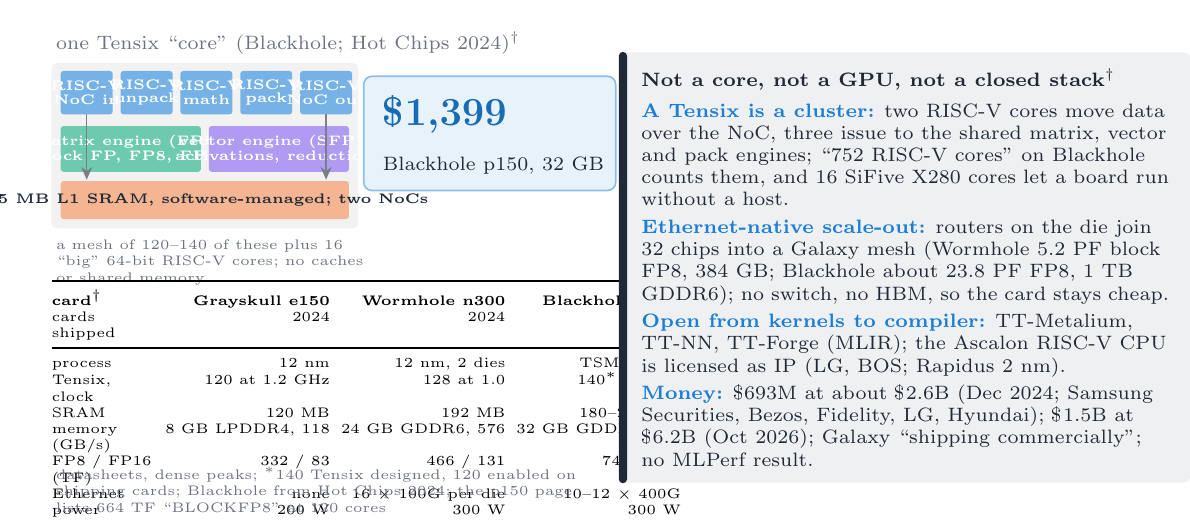
\begin{tikzpicture}
  \useasboundingbox (0,0) rectangle (14.4,5.9);
  \node[lab,anchor=south west] at (0.3,5.5) {one Tensix ``core'' (Blackhole; Hot Chips 2024)$^\dagger$};
  \begin{scope}[shift={(0.3,3.35)}]
    \fill[ink!6,rounded corners=2pt] (0,0) rectangle (3.9,2.1);
    \foreach \i/\lab in {0/{RISC-V\\NoC in},1/{RISC-V\\unpack},2/{RISC-V\\math},3/{RISC-V\\pack},4/{RISC-V\\NoC out}}{
      \fill[mlp!60,rounded corners=1pt] (0.12+\i*0.76,1.45) rectangle ++(0.66,0.55);
      \node[font=\fontsize{4.2}{4.8}\selectfont\bfseries,text=white,align=center] at (0.45+\i*0.76,1.725) {\lab};}
    \fill[emb!60,rounded corners=1pt] (0.12,0.72) rectangle (1.9,1.3);
    \node[font=\fontsize{4.5}{5.3}\selectfont\bfseries,text=white,align=center] at (1.01,1.01) {matrix engine (FPU)\\block FP, FP8, FP16};
    \fill[posc!55,rounded corners=1pt] (2.0,0.72) rectangle (3.78,1.3);
    \node[font=\fontsize{4.5}{5.3}\selectfont\bfseries,text=white,align=center] at (2.89,1.01) {vector engine (SFPU)\\activations, reductions};
    \fill[attn!45,rounded corners=1pt] (0.12,0.12) rectangle (3.78,0.6);
    \node[font=\fontsize{4.3}{5}\selectfont\bfseries,text=ink] at (1.95,0.36) {1.5 MB L1 SRAM, software-managed; two NoCs};
    \draw[thinflow,ink!60] (0.45,1.45) -- (0.45,0.62); \draw[thinflow,ink!60] (3.49,1.45) -- (3.49,0.62);
  \end{scope}
  \node[lab,font=\tiny,anchor=north west,text width=4.2cm] at (0.3,3.27) {a mesh of 120--140 of these plus 16 ``big'' 64-bit RISC-V cores; no caches or shared memory};
  \stat{4.25}{5.3}{\$1{,}399}{Blackhole p150, 32 GB}{mlp}
  \node[anchor=north west,inner sep=0,font=\fontsize{5.1}{6.0}\selectfont] at (0.3,2.7) {%
    \renewcommand{\arraystretch}{0.96}\setlength{\tabcolsep}{2.0pt}%
    \begin{tabular}{@{}>{\raggedright\arraybackslash}p{1.3cm}rrr@{}}
      \toprule
      \textbf{card}$^\dagger$ & \textbf{Grayskull e150} & \textbf{Wormhole n300} & \textbf{Blackhole p150}\\
      cards shipped & 2024 & 2024 & 2025\\
      \midrule
      process & 12 nm & 12 nm, 2 dies & TSMC 6 nm\\
      Tensix, clock & 120 at 1.2 GHz & 128 at 1.0 & 140$^*$ at 1.35\\
      SRAM & 120 MB & 192 MB & 180--210 MB\\
      memory (GB/s) & 8 GB LPDDR4, 118 & 24 GB GDDR6, 576 & 32 GB GDDR6, 512\\
      FP8 / FP16 (TF) & 332 / 83 & 466 / 131 & 745 / 372\\
      Ethernet & none & 16 $\times$ 100G per die & 10--12 $\times$ 400G\\
      power & 200 W & 300 W & 300 W\\
      \bottomrule
    \end{tabular}};
  \node[lab,font=\tiny,anchor=north west,text width=7.0cm] at (0.3,0.38) {datasheets, dense peaks; $^*$140 Tensix designed, 120 enabled on shipping cards; Blackhole from Hot Chips 2024; the p150 page lists 664 TF ``BLOCKFP8'' at 120 cores};
  \bgpanels{7.5}{5.6}{6.7cm}{Not a core, not a GPU, not a closed stack$^\dagger$}{%
    \hl{mlp}{A Tensix is a cluster:} two RISC-V cores move data over
    the NoC, three issue to the shared matrix, vector and pack
    engines; ``752 RISC-V cores'' on Blackhole counts them, and 16
    SiFive X280 cores let a board run without a host.\\[2pt]
    \hl{mlp}{Ethernet-native scale-out:} routers on the die join 32
    chips into a Galaxy mesh (Wormhole 5.2 PF block FP8, 384 GB;
    Blackhole about 23.8 PF FP8, 1 TB GDDR6); no switch, no HBM, so
    the card stays cheap.\\[2pt]
    \hl{mlp}{Open from kernels to compiler:} TT-Metalium, TT-NN,
    TT-Forge (MLIR); the Ascalon RISC-V CPU is licensed as IP (LG,
    BOS; Rapidus 2 nm).\\[2pt]
    \hl{mlp}{Money:} \$693M at about \$2.6B (Dec 2024; Samsung
    Securities, Bezos, Fidelity, LG, Hyundai); \$1.5B at \$6.2B (Oct
    2026); Galaxy ``shipping commercially''; no MLPerf result.}
\end{tikzpicture}
\end{frame}

% ---------------------------------------------------------------- 20
\begin{frame}{Korea's accelerators: Rebellions and FuriosaAI}
\framesubtitle{Latency-first inference chips on Samsung and TSMC 5 nm, then chiplets and HBM; the national fund's picks of 2026.}
\centering
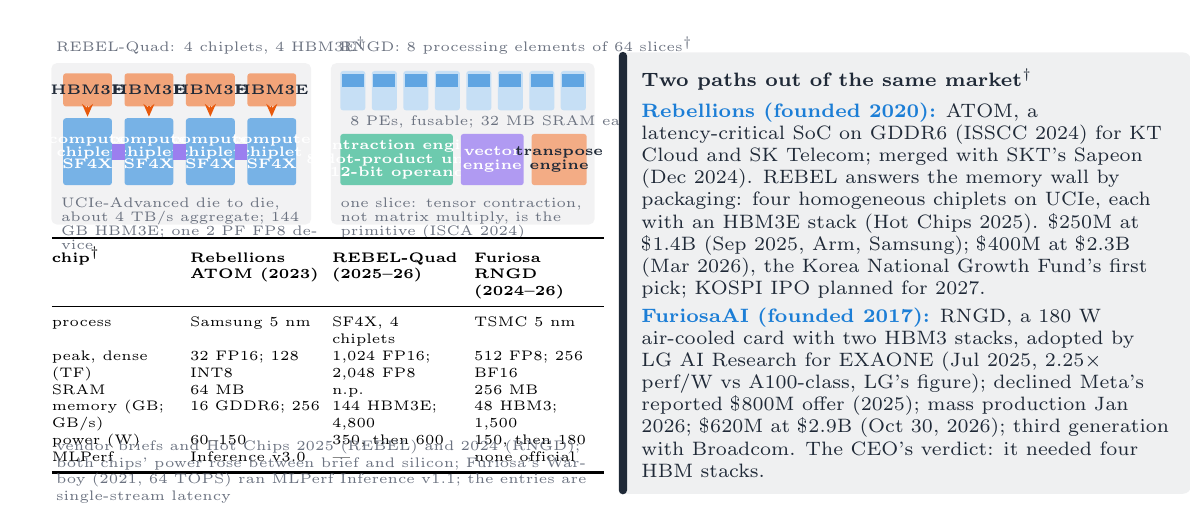
\begin{tikzpicture}
  \useasboundingbox (0,0) rectangle (14.4,5.9);
  \node[lab,anchor=south west,font=\tiny] at (0.3,5.5) {REBEL-Quad: 4 chiplets, 4 HBM3E$^\dagger$};
  \begin{scope}[shift={(0.3,3.4)}]
    \fill[ink!6,rounded corners=2pt] (0,0) rectangle (3.3,2.05);
    \foreach \i in {0,1,2,3}{\fill[attn!55,rounded corners=1pt] (0.15+\i*0.78,1.5) rectangle ++(0.62,0.42);
      \node[font=\fontsize{4}{4.6}\selectfont\bfseries,text=ink] at (0.46+\i*0.78,1.71) {HBM3E};
      \fill[mlp!60,rounded corners=1pt] (0.15+\i*0.78,0.5) rectangle ++(0.62,0.85);
      \node[font=\fontsize{4}{4.6}\selectfont\bfseries,text=white,align=center] at (0.46+\i*0.78,0.925) {compute\\chiplet\\SF4X};
      \draw[thinflow,attn] (0.46+\i*0.78,1.5) -- (0.46+\i*0.78,1.37);}
    \foreach \i in {0,1,2}{\fill[posc!70] (0.77+\i*0.78,0.82) rectangle ++(0.16,0.2);}
    \node[font=\fontsize{4.2}{5}\selectfont,text=muted,anchor=north west,text width=3.3cm] at (0,0.46) {UCIe-Advanced die to die, about 4 TB/s aggregate; 144 GB HBM3E; one 2 PF FP8 device};
  \end{scope}
  \node[lab,anchor=south west,font=\tiny] at (3.9,5.5) {RNGD: 8 processing elements of 64 slices$^\dagger$};
  \begin{scope}[shift={(3.85,3.4)}]
    \fill[ink!6,rounded corners=2pt] (0,0) rectangle (3.35,2.05);
    \foreach \i in {0,...,7}{\fill[mlp!25,rounded corners=1pt] (0.12+\i*0.4,1.45) rectangle ++(0.32,0.5); \fill[mlp!70] (0.14+\i*0.4,1.75) rectangle ++(0.28,0.16);}
    \node[font=\fontsize{4.2}{5}\selectfont,text=muted,anchor=west] at (0.12,1.3) {8 PEs, fusable; 32 MB SRAM each};
    \fill[emb!60,rounded corners=1pt] (0.12,0.5) rectangle (1.55,1.15);
    \node[font=\fontsize{4.2}{4.8}\selectfont\bfseries,text=white,align=center] at (0.835,0.825) {contraction engine\\8 dot-product units\\512-bit operands};
    \fill[posc!55,rounded corners=1pt] (1.65,0.5) rectangle (2.45,1.15);
    \node[font=\fontsize{4.2}{4.8}\selectfont\bfseries,text=white,align=center] at (2.05,0.825) {vector\\engine};
    \fill[attn!50,rounded corners=1pt] (2.55,0.5) rectangle (3.25,1.15);
    \node[font=\fontsize{4.2}{4.8}\selectfont\bfseries,text=ink,align=center] at (2.9,0.825) {transpose\\engine};
    \node[font=\fontsize{4.2}{5}\selectfont,text=muted,anchor=north west,text width=3.35cm] at (0,0.46) {one slice: tensor contraction, not matrix multiply, is the primitive (ISCA 2024)};
  \end{scope}
  \node[anchor=north west,inner sep=0,font=\fontsize{5.2}{6.1}\selectfont] at (0.3,3.25) {%
    \renewcommand{\arraystretch}{1.0}\setlength{\tabcolsep}{2.2pt}%
    \begin{tabular}{@{}>{\raggedright\arraybackslash}p{1.6cm}>{\raggedright\arraybackslash}p{1.65cm}>{\raggedright\arraybackslash}p{1.65cm}>{\raggedright\arraybackslash}p{1.65cm}@{}}
      \toprule
      \textbf{chip}$^\dagger$ & \textbf{Rebellions ATOM (2023)} & \textbf{REBEL-Quad (2025--26)} & \textbf{Furiosa RNGD (2024--26)}\\
      \midrule
      process & Samsung 5 nm & SF4X, 4 chiplets & TSMC 5 nm\\
      peak, dense (TF) & 32 FP16; 128 INT8 & 1{,}024 FP16; 2{,}048 FP8 & 512 FP8; 256 BF16\\
      SRAM & 64 MB & n.p. & 256 MB\\
      memory (GB; GB/s) & 16 GDDR6; 256 & 144 HBM3E; 4{,}800 & 48 HBM3; 1{,}500\\
      power (W) & 60--150 & 350, then 600 & 150, then 180\\
      MLPerf & Inference v3.0 & --- & none official\\
      \bottomrule
    \end{tabular}};
  \node[lab,font=\tiny,anchor=north west,text width=7.0cm] at (0.3,0.72) {vendor briefs and Hot Chips 2025 (REBEL) and 2024 (RNGD); both chips' power rose between brief and silicon; Furiosa's Warboy (2021, 64 TOPS) ran MLPerf Inference v1.1; the entries are single-stream latency};
  \bgpanels{7.5}{5.6}{6.7cm}{Two paths out of the same market$^\dagger$}{%
    \hl{mlp}{Rebellions (founded 2020):} ATOM, a latency-critical
    SoC on GDDR6 (ISSCC 2024) for KT Cloud and SK Telecom; merged
    with SKT's Sapeon (Dec 2024). REBEL answers the memory wall by
    packaging: four homogeneous chiplets on UCIe, each with an HBM3E
    stack (Hot Chips 2025). \$250M at \$1.4B (Sep 2025, Arm, Samsung);
    \$400M at \$2.3B (Mar 2026), the Korea National Growth Fund's
    first pick; KOSPI IPO planned for 2027.\\[2pt]
    \hl{mlp}{FuriosaAI (founded 2017):} RNGD, a 180 W air-cooled card
    with two HBM3 stacks, adopted by LG AI Research for EXAONE (Jul
    2025, 2.25$\times$ perf/W vs A100-class, LG's figure); declined
    Meta's reported \$800M offer (2025); mass production Jan 2026;
    \$620M at \$2.9B (Oct 30, 2026); third generation with Broadcom.
    The CEO's verdict: it needed four HBM stacks.}
\end{tikzpicture}
\end{frame}

% ---------------------------------------------------------------- 21
\stage{6}
\begin{frame}{AWS Inferentia and Trainium: captive volume, four generations}
\framesubtitle{A systolic NeuronCore, HBM and a torus; UltraServers reach 144 chips, and Anthropic's Rainier runs 500,000.}
\centering
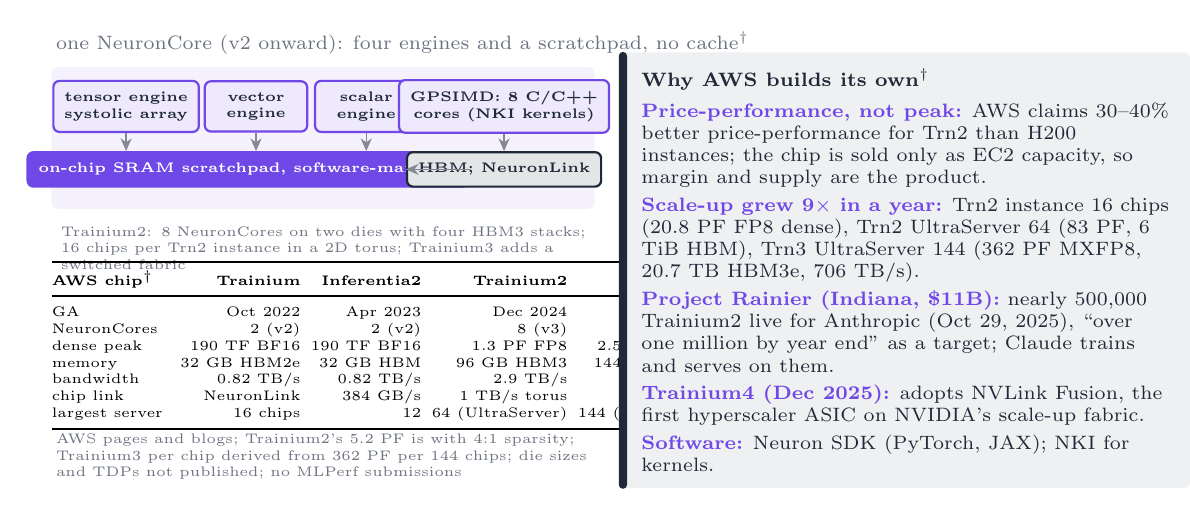
\begin{tikzpicture}
  \useasboundingbox (0,0) rectangle (14.4,5.9);
  % NeuronCore block diagram
  \node[lab,anchor=south west] at (0.3,5.5) {one NeuronCore (v2 onward): four engines and a scratchpad, no cache$^\dagger$};
  \begin{scope}[shift={(0.3,3.6)}]
    \fill[posc!7,rounded corners=2pt] (0,0) rectangle (6.9,1.8);
    \node[comp=posc,minimum width=1.55cm,minimum height=0.6cm,font=\fontsize{5}{6}\selectfont\bfseries,text=ink,align=center] (te) at (0.95,1.3) {tensor engine\\systolic array};
    \node[comp=posc,minimum width=1.3cm,minimum height=0.6cm,font=\fontsize{5}{6}\selectfont\bfseries,text=ink,align=center] (ve) at (2.6,1.3) {vector\\engine};
    \node[comp=posc,minimum width=1.3cm,minimum height=0.6cm,font=\fontsize{5}{6}\selectfont\bfseries,text=ink,align=center] (se) at (4.0,1.3) {scalar\\engine};
    \node[comp=posc,minimum width=1.75cm,minimum height=0.6cm,font=\fontsize{5}{6}\selectfont\bfseries,text=ink,align=center] (gp) at (5.75,1.3) {GPSIMD: 8 C/C++\\cores (NKI kernels)};
    \node[comp=posc,minimum width=4.5cm,minimum height=0.4cm,font=\fontsize{5}{6}\selectfont\bfseries,text=white,fill=posc,align=center] (sb) at (2.5,0.5) {on-chip SRAM scratchpad, software-managed};
    \node[comp=ink,minimum width=1.75cm,minimum height=0.4cm,font=\fontsize{5}{6}\selectfont\bfseries,text=ink,align=center] (hbm) at (5.75,0.5) {HBM; NeuronLink};
    \foreach \e in {te,ve,se}{\draw[thinflow] (\e.south) -- (\e.south|-sb.north);}
    \draw[thinflow] (gp.south) -- (gp.south|-hbm.north);
    \draw[thinflow] (sb) -- (hbm);
  \end{scope}
  \node[font=\tiny,text=muted,anchor=north west,text width=6.9cm] at (0.3,3.5) {Trainium2: 8 NeuronCores on two dies with four HBM3 stacks; 16 chips per Trn2 instance in a 2D torus; Trainium3 adds a switched fabric};
  \node[anchor=north west,inner sep=0,font=\fontsize{5.1}{6.1}\selectfont] at (0.3,2.95) {%
    \renewcommand{\arraystretch}{1.0}\setlength{\tabcolsep}{1.9pt}%
    \begin{tabular}{@{}>{\raggedright\arraybackslash}p{1.5cm}rrrr@{}}
      \toprule
      \textbf{AWS chip}$^\dagger$ & \textbf{Trainium} & \textbf{Inferentia2} & \textbf{Trainium2} & \textbf{Trainium3}\\
      \midrule
      GA & Oct 2022 & Apr 2023 & Dec 2024 & Dec 2025\\
      NeuronCores & 2 (v2) & 2 (v2) & 8 (v3) & 8 $+$ comm.\\
      dense peak & 190 TF BF16 & 190 TF BF16 & 1.3 PF FP8 & 2.5 PF MXFP8\\
      memory & 32 GB HBM2e & 32 GB HBM & 96 GB HBM3 & 144 GB HBM3e\\
      bandwidth & 0.82 TB/s & 0.82 TB/s & 2.9 TB/s & 4.9 TB/s\\
      chip link & NeuronLink & 384 GB/s & 1 TB/s torus & 2.6 TB/s\\
      largest server & 16 chips & 12 & 64 (UltraServer) & 144 (UltraServer)\\
      \bottomrule
    \end{tabular}};
  \node[lab,font=\tiny,anchor=north west,text width=7.0cm] at (0.3,0.8) {AWS pages and blogs; Trainium2's 5.2 PF is with 4:1 sparsity; Trainium3 per chip derived from 362 PF per 144 chips; die sizes and TDPs not published; no MLPerf submissions};
  \bgpanels{7.5}{5.6}{6.7cm}{Why AWS builds its own$^\dagger$}{%
    \hl{posc}{Price-performance, not peak:} AWS claims 30--40\% better
    price-performance for Trn2 than H200 instances; the chip is sold
    only as EC2 capacity, so margin and supply are the product.\\[2pt]
    \hl{posc}{Scale-up grew 9$\times$ in a year:} Trn2 instance 16 chips
    (20.8 PF FP8 dense), Trn2 UltraServer 64 (83 PF, 6 TiB HBM), Trn3
    UltraServer 144 (362 PF MXFP8, 20.7 TB HBM3e, 706 TB/s).\\[2pt]
    \hl{posc}{Project Rainier (Indiana, \$11B):} nearly 500{,}000
    Trainium2 live for Anthropic (Oct 29, 2025), ``over one million
    by year end'' as a target; Claude trains and serves on them.\\[2pt]
    \hl{posc}{Trainium4 (Dec 2025):} adopts NVLink Fusion, the first
    hyperscaler ASIC on NVIDIA's scale-up fabric.\\[2pt]
    \hl{posc}{Software:} Neuron SDK (PyTorch, JAX); NKI for kernels.}
\end{tikzpicture}
\end{frame}

% ---------------------------------------------------------------- 22
\begin{frame}{Microsoft Maia and Meta MTIA: inference first, then everything}
\framesubtitle{Maia runs on Ethernet; MTIA grew from a 25 W recommendation chip into a 1.7 kW HBM part in three years.}
\centering
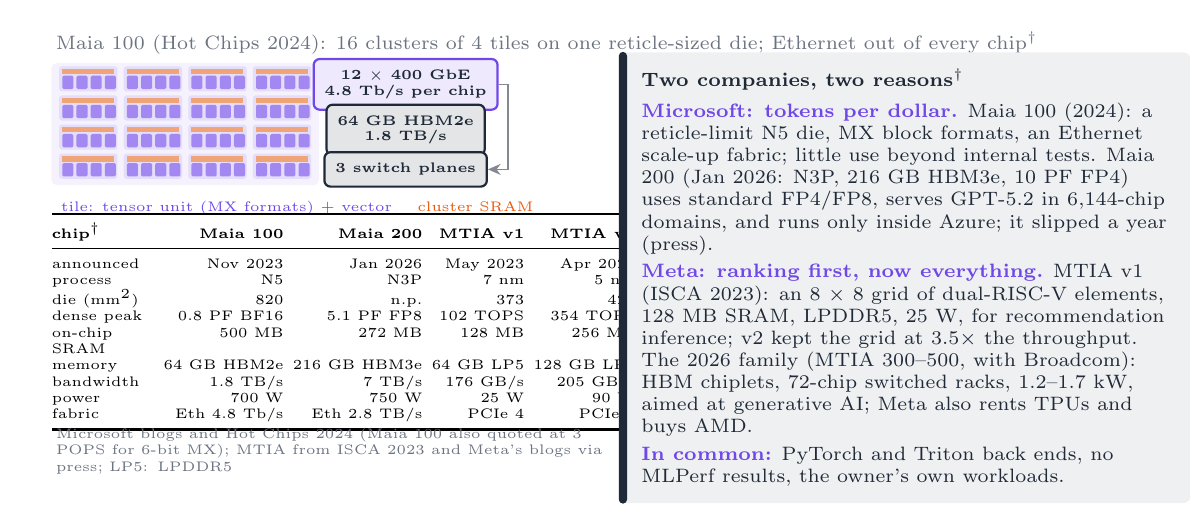
\begin{tikzpicture}
  \useasboundingbox (0,0) rectangle (14.4,5.9);
  \node[lab,anchor=south west] at (0.3,5.5) {Maia 100 (Hot Chips 2024): 16 clusters of 4 tiles on one reticle-sized die; Ethernet out of every chip$^\dagger$};
  \begin{scope}[shift={(0.3,3.9)}]
    \fill[posc!7,rounded corners=2pt] (0,0) rectangle (3.4,1.55);
    \foreach \c in {0,...,3}{\foreach \r in {0,...,3}{
      \fill[posc!18,rounded corners=1pt] (0.1+\c*0.82,0.08+\r*0.37) rectangle ++(0.74,0.32);
      \foreach \t in {0,...,3}{\fill[posc!65,rounded corners=0.5pt] (0.14+\c*0.82+\t*0.18,0.11+\r*0.37) rectangle ++(0.14,0.17);}
      \fill[attn!55] (0.14+\c*0.82,0.3+\r*0.37) rectangle ++(0.66,0.07);}}
    \begin{scope}[shift={(3.7,0)}]
      \node[comp=posc,minimum width=1.45cm,minimum height=0.46cm,font=\fontsize{4.8}{5.6}\selectfont\bfseries,text=ink,align=center] (nic) at (0.8,1.28) {12 $\times$ 400 GbE\\4.8 Tb/s per chip};
      \node[comp=ink,minimum width=1.45cm,minimum height=0.46cm,font=\fontsize{4.8}{5.6}\selectfont\bfseries,text=ink,align=center] (hb) at (0.8,0.7) {64 GB HBM2e\\1.8 TB/s};
      \node[comp=ink,minimum width=1.45cm,minimum height=0.36cm,font=\fontsize{4.8}{5.6}\selectfont\bfseries,text=ink,align=center] (sw) at (0.8,0.2) {3 switch planes};
      \draw[thinflow] (nic.east) -- ++(0.12,0) |- (sw.east);
    \end{scope}
  \end{scope}
  \node[font=\fontsize{4.6}{5.4}\selectfont,text=ink,anchor=north west] at (0.3,3.82) {\textcolor{posc}{tile: tensor unit (MX formats) $+$ vector} \quad \textcolor{attn}{cluster SRAM}};
  \node[anchor=north west,inner sep=0,font=\fontsize{4.9}{5.9}\selectfont] at (0.3,3.55) {%
    \renewcommand{\arraystretch}{1.0}\setlength{\tabcolsep}{1.7pt}%
    \begin{tabular}{@{}>{\raggedright\arraybackslash}p{1.3cm}rrrrr@{}}
      \toprule
      \textbf{chip}$^\dagger$ & \textbf{Maia 100} & \textbf{Maia 200} & \textbf{MTIA v1} & \textbf{MTIA v2} & \textbf{MTIA 400}\\
      \midrule
      announced & Nov 2023 & Jan 2026 & May 2023 & Apr 2024 & Mar 2026\\
      process & N5 & N3P & 7 nm & 5 nm & chiplets\\
      die (mm$^2$) & 820 & n.p. & 373 & 421 & ---\\
      dense peak & 0.8 PF BF16 & 5.1 PF FP8 & 102 TOPS & 354 TOPS & 6 PF FP8\\
      on-chip SRAM & 500 MB & 272 MB & 128 MB & 256 MB & n.p.\\
      memory & 64 GB HBM2e & 216 GB HBM3e & 64 GB LP5 & 128 GB LP5 & 288 GB HBM\\
      bandwidth & 1.8 TB/s & 7 TB/s & 176 GB/s & 205 GB/s & 9.2 TB/s\\
      power & 700 W & 750 W & 25 W & 90 W & 1{,}200 W\\
      fabric & Eth 4.8 Tb/s & Eth 2.8 TB/s & PCIe 4 & PCIe 5 & 72/rack\\
      \bottomrule
    \end{tabular}};
  \node[lab,font=\tiny,anchor=north west,text width=7.0cm] at (0.3,0.88) {Microsoft blogs and Hot Chips 2024 (Maia 100 also quoted at 3 POPS for 6-bit MX); MTIA from ISCA 2023 and Meta's blogs via press; LP5: LPDDR5};
  \bgpanels{7.5}{5.6}{6.7cm}{Two companies, two reasons$^\dagger$}{%
    \hl{posc}{Microsoft: tokens per dollar.} Maia 100 (2024): a
    reticle-limit N5 die, MX block formats, an Ethernet scale-up
    fabric; little use beyond internal tests. Maia 200 (Jan 2026:
    N3P, 216 GB HBM3e, 10 PF FP4) uses standard FP4/FP8, serves
    GPT-5.2 in 6{,}144-chip domains, and runs only inside Azure;
    it slipped a year (press).\\[2pt]
    \hl{posc}{Meta: ranking first, now everything.} MTIA v1 (ISCA
    2023): an 8 $\times$ 8 grid of dual-RISC-V elements, 128 MB SRAM,
    LPDDR5, 25 W, for recommendation inference; v2 kept the grid at
    3.5$\times$ the throughput. The 2026 family (MTIA 300--500, with
    Broadcom): HBM chiplets, 72-chip switched racks, 1.2--1.7 kW,
    aimed at generative AI; Meta also rents TPUs and buys AMD.\\[2pt]
    \hl{posc}{In common:} PyTorch and Triton back ends, no MLPerf
    results, the owner's own workloads.}
\end{tikzpicture}
\end{frame}

% ---------------------------------------------------------------- 23
\begin{frame}{OpenAI--Broadcom and the custom-XPU model}
\framesubtitle{The buyer owns the architecture, Broadcom the silicon and SerDes, TSMC the wafers; 10 GW for OpenAI by 2029.}
\centering
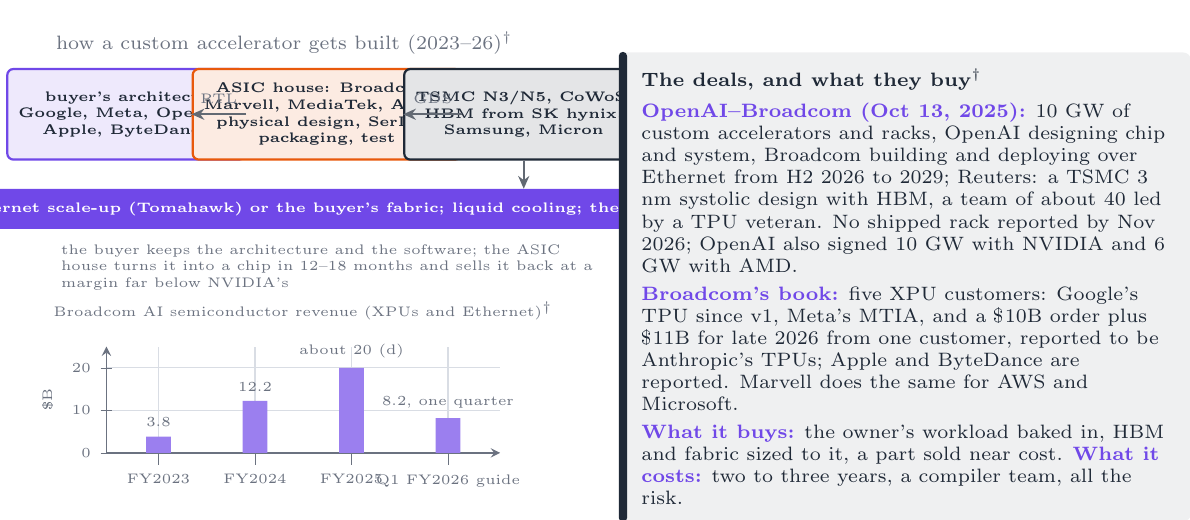
\begin{tikzpicture}
  \useasboundingbox (0,0) rectangle (14.4,5.9);
  \node[lab,anchor=south west] at (0.3,5.5) {how a custom accelerator gets built (2023--26)$^\dagger$};
  \begin{scope}[shift={(0.3,2.85)}]
    \node[comp=posc,minimum width=1.8cm,minimum height=1.15cm,font=\fontsize{5}{6}\selectfont\bfseries,text=ink,align=center] (buyer) at (0.95,1.95) {buyer's architects\\Google, Meta, OpenAI,\\Apple, ByteDance};
    \node[comp=attn,minimum width=1.8cm,minimum height=1.15cm,font=\fontsize{5}{6}\selectfont\bfseries,text=ink,align=center] (bcm) at (3.5,1.95) {ASIC house: Broadcom,\\Marvell, MediaTek, Alchip\\physical design, SerDes,\\packaging, test};
    \node[comp=ink,minimum width=1.8cm,minimum height=1.15cm,font=\fontsize{5}{6}\selectfont\bfseries,text=ink,align=center] (fab) at (6.0,1.95) {TSMC N3/N5, CoWoS;\\HBM from SK hynix,\\Samsung, Micron};
    \draw[flow] (buyer) -- node[above,font=\fontsize{4.5}{5}\selectfont,text=muted] {RTL} (bcm);
    \draw[flow] (bcm) -- node[above,font=\fontsize{4.5}{5}\selectfont,text=muted] {GDS} (fab);
    \node[comp=posc,minimum width=6.7cm,minimum height=0.48cm,font=\fontsize{5}{6}\selectfont\bfseries,text=white,fill=posc,align=center] (rack) at (3.5,0.75) {rack: Ethernet scale-up (Tomahawk) or the buyer's fabric; liquid cooling; the buyer's cloud};
    \draw[flow] (fab.south) -- (fab.south|-rack.north);
    \node[font=\tiny,text=muted,anchor=north west,text width=6.8cm] at (0,0.42) {the buyer keeps the architecture and the software; the ASIC house turns it into a chip in 12--18 months and sells it back at a margin far below NVIDIA's};
  \end{scope}
  \begin{scope}[shift={(1.0,0.5)}]
  \begin{axis}[lecture,scale only axis,width=5.0cm,height=1.35cm,ybar,bar width=9pt,ymin=0,ymax=25,enlarge x limits=0.18,
      symbolic x coords={FY2023,FY2024,FY2025,Q1 FY2026 guide},xtick={FY2023,FY2024,FY2025,Q1 FY2026 guide},xticklabel style={font=\tiny},
      ylabel={\$B},ylabel style={font=\tiny},ytick={0,10,20},yticklabel style={font=\tiny},
      nodes near coords,nodes near coords style={font=\tiny,text=muted},point meta=explicit symbolic,
      title style={font=\tiny,text=muted,at={(0.5,1.0)}},title={Broadcom AI semiconductor revenue (XPUs and Ethernet)$^\dagger$}]
    \addplot[fill=posc!70,draw=none] coordinates {(FY2023,3.8)[3.8] (FY2024,12.2)[12.2] (FY2025,20)[about 20 (d)] ({Q1 FY2026 guide},8.2)[8.2, one quarter]};
  \end{axis}
  \end{scope}
  \bgpanels{7.5}{5.6}{6.7cm}{The deals, and what they buy$^\dagger$}{%
    \hl{posc}{OpenAI--Broadcom (Oct 13, 2025):} 10 GW of custom
    accelerators and racks, OpenAI designing chip and system,
    Broadcom building and deploying over Ethernet from H2 2026 to
    2029; Reuters: a TSMC 3 nm systolic design with HBM, a team of
    about 40 led by a TPU veteran. No shipped rack reported by Nov
    2026; OpenAI also signed 10 GW with NVIDIA and 6 GW with AMD.\\[2pt]
    \hl{posc}{Broadcom's book:} five XPU customers: Google's TPU since
    v1, Meta's MTIA, and a \$10B order plus \$11B for late 2026 from
    one customer, reported to be Anthropic's TPUs; Apple and ByteDance
    are reported. Marvell does the same for AWS and Microsoft.\\[2pt]
    \hl{posc}{What it buys:} the owner's workload baked in, HBM and
    fabric sized to it, a part sold near cost. \hl{posc}{What it
    costs:} two to three years, a compiler team, all the risk.}
\end{tikzpicture}
\end{frame}

% ---------------------------------------------------------------- 24
\begin{frame}{The established vendors: Gaudi, Cloud AI, Spyre, Dojo}
\framesubtitle{Intel bought one line and killed another; Qualcomm bets on LPDDR; IBM sits beside the mainframe; Tesla paused.}
\centering
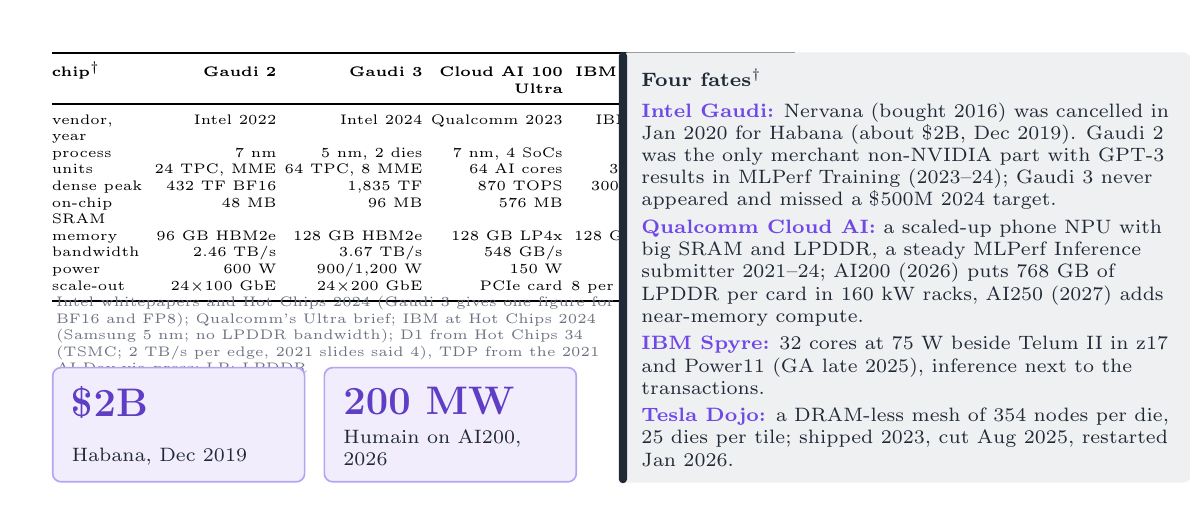
\begin{tikzpicture}
  \useasboundingbox (0,0) rectangle (14.4,5.9);
  \node[anchor=north west,inner sep=0,font=\fontsize{4.9}{5.9}\selectfont] at (0.3,5.6) {%
    \renewcommand{\arraystretch}{1.02}\setlength{\tabcolsep}{1.5pt}%
    \begin{tabular}{@{}>{\raggedright\arraybackslash}p{1.2cm}rrrrr@{}}
      \toprule
      \textbf{chip}$^\dagger$ & \textbf{Gaudi 2} & \textbf{Gaudi 3} & \textbf{Cloud AI 100} & \textbf{IBM Spyre} & \textbf{Tesla D1}\\
       & & & \textbf{Ultra} & & \\
      \midrule
      vendor, year & Intel 2022 & Intel 2024 & Qualcomm 2023 & IBM 2025 & Tesla 2021\\
      process & 7 nm & 5 nm, 2 dies & 7 nm, 4 SoCs & 5 nm & 7 nm\\
      units & 24 TPC, MME & 64 TPC, 8 MME & 64 AI cores & 32 cores & 354 nodes\\
      dense peak & 432 TF BF16 & 1{,}835 TF & 870 TOPS & 300 TOPS & 362 TF BF16\\
      on-chip SRAM & 48 MB & 96 MB & 576 MB & 64 MB & 440 MB\\
      memory & 96 GB HBM2e & 128 GB HBM2e & 128 GB LP4x & 128 GB LP5 & none on die\\
      bandwidth & 2.46 TB/s & 3.67 TB/s & 548 GB/s & n.p. & 2 TB/s edge\\
      power & 600 W & 900/1{,}200 W & 150 W & 75 W & 400 W\\
      scale-out & 24$\times$100 GbE & 24$\times$200 GbE & PCIe card & 8 per drawer & 25-die tile\\
      \bottomrule
    \end{tabular}};
  \node[lab,font=\tiny,anchor=north west,text width=7.1cm] at (0.3,2.55) {Intel whitepapers and Hot Chips 2024 (Gaudi 3 gives one figure for BF16 and FP8); Qualcomm's Ultra brief; IBM at Hot Chips 2024 (Samsung 5 nm; no LPDDR bandwidth); D1 from Hot Chips 34 (TSMC; 2 TB/s per edge, 2021 slides said 4), TDP from the 2021 AI Day via press; LP: LPDDR};
  \stat{0.3}{1.6}{\$2B}{Habana, Dec 2019}{posc}
  \stat{3.75}{1.6}{200 MW}{Humain on AI200, 2026}{posc}
  \bgpanels{7.5}{5.6}{6.7cm}{Four fates$^\dagger$}{%
    \hl{posc}{Intel Gaudi:} Nervana (bought 2016) was cancelled in
    Jan 2020 for Habana (about \$2B, Dec 2019). Gaudi 2 was the only
    merchant non-NVIDIA part with GPT-3 results in MLPerf Training (2023--24);
    Gaudi 3 never appeared and missed
    a \$500M 2024 target.\\[2pt]
    \hl{posc}{Qualcomm Cloud AI:} a scaled-up phone NPU with big SRAM
    and LPDDR, a steady MLPerf Inference submitter 2021--24; AI200
    (2026) puts 768 GB of LPDDR per card in 160 kW racks, AI250
    (2027) adds near-memory compute.\\[2pt]
    \hl{posc}{IBM Spyre:} 32 cores at 75 W beside Telum II in z17 and
    Power11 (GA late 2025), inference next to the transactions.\\[2pt]
    \hl{posc}{Tesla Dojo:} a DRAM-less mesh of 354 nodes per die,
    25 dies per tile; shipped 2023, cut Aug 2025, restarted Jan 2026.}
\end{tikzpicture}
\end{frame}

% ---------------------------------------------------------------- 25
\stage{7}
\begin{frame}{Huawei Ascend: Da Vinci cores to the 950/960/970 roadmap}
\framesubtitle{Cube-MAC cores on 7 nm; cut off from TSMC in 2020, Huawei designs its own HBM and scales by count.}
\centering
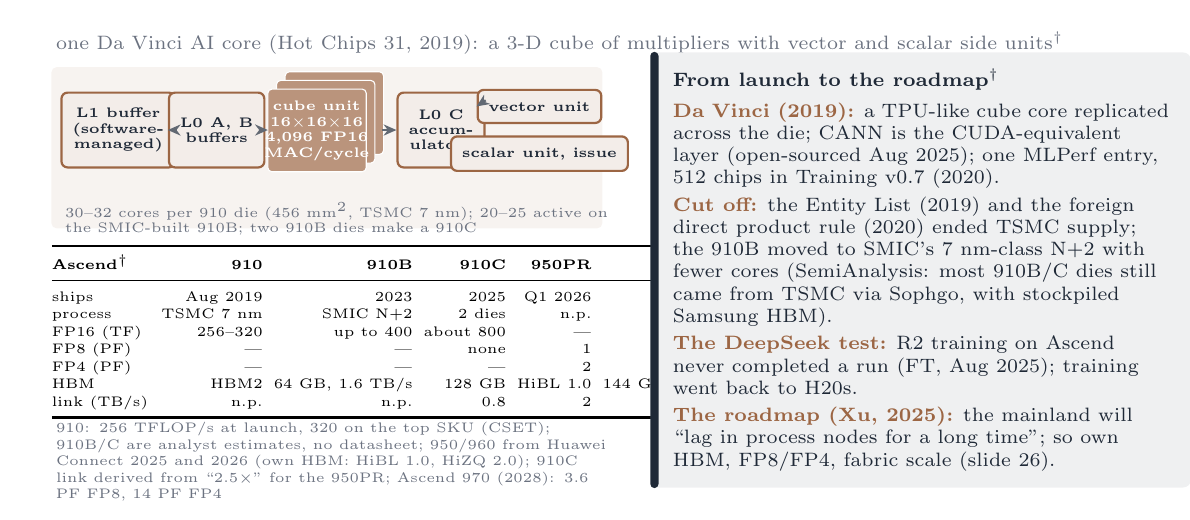
\begin{tikzpicture}
  \useasboundingbox (0,0) rectangle (14.4,5.9);
  \node[lab,anchor=south west] at (0.3,5.5) {one Da Vinci AI core (Hot Chips 31, 2019): a 3-D cube of multipliers with vector and scalar side units$^\dagger$};
  \begin{scope}[shift={(0.3,3.35)}]
    \fill[trn!8,rounded corners=2pt] (0,0) rectangle (7.0,2.05);
    \node[comp=trn,minimum width=1.25cm,minimum height=0.95cm,font=\fontsize{4.8}{5.6}\selectfont\bfseries,text=ink,align=center] (l1) at (0.85,1.25) {L1 buffer\\(software-\\managed)};
    \node[comp=trn,minimum width=0.9cm,minimum height=0.95cm,font=\fontsize{4.6}{5.4}\selectfont\bfseries,text=ink,align=center] (l0) at (2.1,1.25) {L0 A, B\\buffers};
    % cube: three stacked squares to suggest 16x16x16
    \foreach \d in {0.22,0.11,0}{\fill[trn!70,rounded corners=1.5pt,draw=white,line width=0.4pt] (2.75+\d,0.72+\d) rectangle ++(1.25,1.05);}
    \node[font=\fontsize{4.8}{5.6}\selectfont\bfseries,text=white,align=center] at (3.37,1.24) {cube unit\\16$\times$16$\times$16\\4{,}096 FP16\\MAC/cycle};
    \node[comp=trn,minimum width=0.95cm,minimum height=0.95cm,font=\fontsize{4.6}{5.4}\selectfont\bfseries,text=ink,align=center] (l0c) at (4.95,1.25) {L0 C\\accum-\\ulators};
    \node[comp=trn,minimum width=1.3cm,minimum height=0.42cm,font=\fontsize{4.6}{5.4}\selectfont\bfseries,text=ink,align=center] (vec) at (6.2,1.55) {vector unit};
    \node[comp=trn,minimum width=1.3cm,minimum height=0.42cm,font=\fontsize{4.6}{5.4}\selectfont\bfseries,text=ink,align=center] (sca) at (6.2,0.95) {scalar unit, issue};
    \draw[flow] (l1) -- (l0); \draw[flow] (l0) -- (2.75,1.25); \draw[flow] (4.2,1.25) -- (l0c); \draw[flow] (l0c) -- (vec.west);
    \node[font=\fontsize{4.6}{5.4}\selectfont,text=muted,anchor=north west,text width=6.9cm] at (0.05,0.45) {30--32 cores per 910 die (456 mm$^2$, TSMC 7 nm); 20--25 active on the SMIC-built 910B; two 910B dies make a 910C};
  \end{scope}
  \node[anchor=north west,inner sep=0,font=\fontsize{5.2}{6.2}\selectfont] at (0.3,3.15) {%
    \renewcommand{\arraystretch}{1.02}\setlength{\tabcolsep}{2.0pt}%
    \begin{tabular}{@{}>{\raggedright\arraybackslash}p{1.25cm}rrrrrr@{}}
      \toprule
      \textbf{Ascend}$^\dagger$ & \textbf{910} & \textbf{910B} & \textbf{910C} & \textbf{950PR} & \textbf{950DT} & \textbf{960}\\
      \midrule
      ships & Aug 2019 & 2023 & 2025 & Q1 2026 & Q4 2026 & Q1 2027\\
      process & TSMC 7 nm & SMIC N$+$2 & 2 dies & n.p. & same die & n.p.\\
      FP16 (TF) & 256--320 & up to 400 & about 800 & --- & --- & ---\\
      FP8 (PF) & --- & --- & none & 1 & 1 & 2\\
      FP4 (PF) & --- & --- & --- & 2 & 2 & 8 (PR)\\
      HBM & HBM2 & 64 GB, 1.6 TB/s & 128 GB & HiBL 1.0 & 144 GB, 4 TB/s & about 2$\times$\\
      link (TB/s) & n.p. & n.p. & 0.8 & 2 & 2 & 2.2\\
      \bottomrule
    \end{tabular}};
  \node[lab,font=\tiny,anchor=north west,text width=7.0cm] at (0.3,0.95) {910: 256 TFLOP/s at launch, 320 on the top SKU (CSET); 910B/C are analyst estimates, no datasheet; 950/960 from Huawei Connect 2025 and 2026 (own HBM: HiBL 1.0, HiZQ 2.0); 910C link derived from ``2.5$\times$'' for the 950PR; Ascend 970 (2028): 3.6 PF FP8, 14 PF FP4};
  \bgpanels{7.9}{5.6}{6.3cm}{From launch to the roadmap$^\dagger$}{%
    \hl{trn}{Da Vinci (2019):} a TPU-like cube core replicated
    across the die; CANN is the CUDA-equivalent layer (open-sourced
    Aug 2025); one MLPerf entry, 512 chips in Training v0.7 (2020).\\[2pt]
    \hl{trn}{Cut off:} the Entity List (2019) and the foreign direct
    product rule (2020) ended TSMC supply; the 910B moved to SMIC's
    7 nm-class N$+$2 with fewer cores (SemiAnalysis: most 910B/C dies
    still came from TSMC via Sophgo, with stockpiled Samsung HBM).\\[2pt]
    \hl{trn}{The DeepSeek test:} R2 training on Ascend never
    completed a run (FT, Aug 2025); training went back to H20s.\\[2pt]
    \hl{trn}{The roadmap (Xu, 2025):} the mainland will ``lag in
    process nodes for a long time''; so own HBM, FP8/FP4, fabric
    scale (slide 26).}
\end{tikzpicture}
\end{frame}

% ---------------------------------------------------------------- 26
\begin{frame}{CloudMatrix 384 and the SuperPoDs: scale, not per-chip speed}
\framesubtitle{384 Ascend 910C on an all-optical fabric out-total a GB200 NVL72 at about four times the power.}
\centering
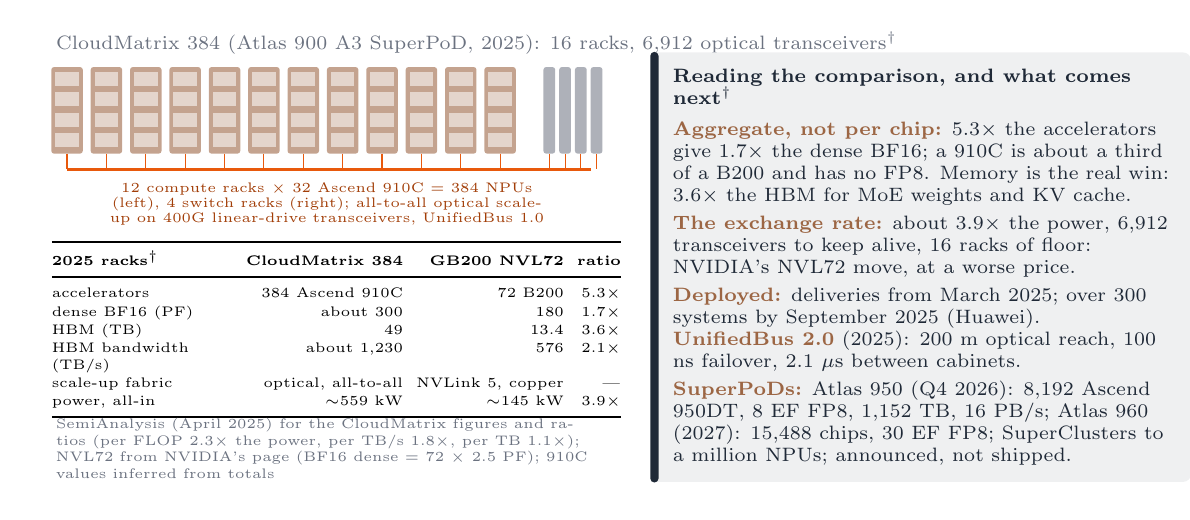
\begin{tikzpicture}
  \useasboundingbox (0,0) rectangle (14.4,5.9);
  \node[lab,anchor=south west] at (0.3,5.5) {CloudMatrix 384 (Atlas 900 A3 SuperPoD, 2025): 16 racks, 6{,}912 optical transceivers$^\dagger$};
  \begin{scope}[shift={(0.3,3.55)}]
    \foreach \i in {0,...,11}{\fill[trn!60,rounded corners=1pt] (\i*0.5,0.75) rectangle ++(0.4,1.1);
      \foreach \k in {0,...,3}{\fill[white,opacity=0.55] (\i*0.5+0.05,0.83+\k*0.26) rectangle ++(0.3,0.18);}}
    \foreach \i in {0,...,3}{\fill[muted!55,rounded corners=1pt] (6.25+\i*0.2,0.75) rectangle ++(0.15,1.1);}
    \draw[attn,line width=0.9pt] (0.2,0.55) -- (6.85,0.55);
    \foreach \i in {0,...,11}{\draw[attn,line width=0.4pt] (\i*0.5+0.2,0.75) -- (\i*0.5+0.2,0.55);}
    \foreach \i in {0,...,3}{\draw[attn,line width=0.4pt] (6.325+\i*0.2,0.75) -- (6.325+\i*0.2,0.55);}
    \node[font=\fontsize{4.6}{5.4}\selectfont,text=attn!70!black,anchor=north,text width=7.0cm,align=center] at (3.5,0.5) {12 compute racks $\times$ 32 Ascend 910C $=$ 384 NPUs (left), 4 switch racks (right); all-to-all optical scale-up on 400G linear-drive transceivers, UnifiedBus 1.0};
  \end{scope}
  \node[anchor=north west,inner sep=0,font=\fontsize{5.4}{6.4}\selectfont] at (0.3,3.2) {%
    \renewcommand{\arraystretch}{1.02}\setlength{\tabcolsep}{2.4pt}%
    \begin{tabular}{@{}>{\raggedright\arraybackslash}p{2.3cm}rrr@{}}
      \toprule
      \textbf{2025 racks}$^\dagger$ & \textbf{CloudMatrix 384} & \textbf{GB200 NVL72} & \textbf{ratio}\\
      \midrule
      accelerators & 384 Ascend 910C & 72 B200 & 5.3$\times$\\
      dense BF16 (PF) & about 300 & 180 & 1.7$\times$\\
      HBM (TB) & 49 & 13.4 & 3.6$\times$\\
      HBM bandwidth (TB/s) & about 1{,}230 & 576 & 2.1$\times$\\
      scale-up fabric & optical, all-to-all & NVLink 5, copper & ---\\
      power, all-in & ${\sim}$559 kW & ${\sim}$145 kW & 3.9$\times$\\
      \bottomrule
    \end{tabular}};
  \node[lab,font=\tiny,anchor=north west,text width=7.0cm] at (0.3,1.0) {SemiAnalysis (April 2025) for the CloudMatrix figures and ratios (per FLOP 2.3$\times$ the power, per TB/s 1.8$\times$, per TB 1.1$\times$); NVL72 from NVIDIA's page (BF16 dense $=$ 72 $\times$ 2.5 PF); 910C values inferred from totals};
  \bgpanels{7.9}{5.6}{6.3cm}{Reading the comparison, and what comes next$^\dagger$}{%
    \hl{trn}{Aggregate, not per chip:} 5.3$\times$ the accelerators
    give 1.7$\times$ the dense BF16; a 910C is about a third of a
    B200 and has no FP8. Memory is the real win: 3.6$\times$ the HBM
    for MoE weights and KV cache.\\[2pt]
    \hl{trn}{The exchange rate:} about 3.9$\times$ the power, 6{,}912
    transceivers to keep alive, 16 racks of floor: NVIDIA's NVL72
    move, at a worse price.\\[2pt]
    \hl{trn}{Deployed:} deliveries from March 2025; over 300 systems
    by September 2025 (Huawei). \hl{trn}{UnifiedBus 2.0} (2025):
    200 m optical reach, 100 ns failover, 2.1 $\mu$s between
    cabinets.\\[2pt]
    \hl{trn}{SuperPoDs:} Atlas 950 (Q4 2026): 8{,}192 Ascend 950DT,
    8 EF FP8, 1{,}152 TB, 16 PB/s; Atlas 960 (2027): 15{,}488
    chips, 30 EF FP8; SuperClusters to a million NPUs; announced,
    not shipped.}
\end{tikzpicture}
\end{frame}

% ---------------------------------------------------------------- 27
\begin{frame}{Kunlun, Hanguang, Cambricon and the policy backdrop}
\framesubtitle{China's ASIC lines, its GPU-like rivals' IPO wave, and the export-control calendar behind both.}
\centering
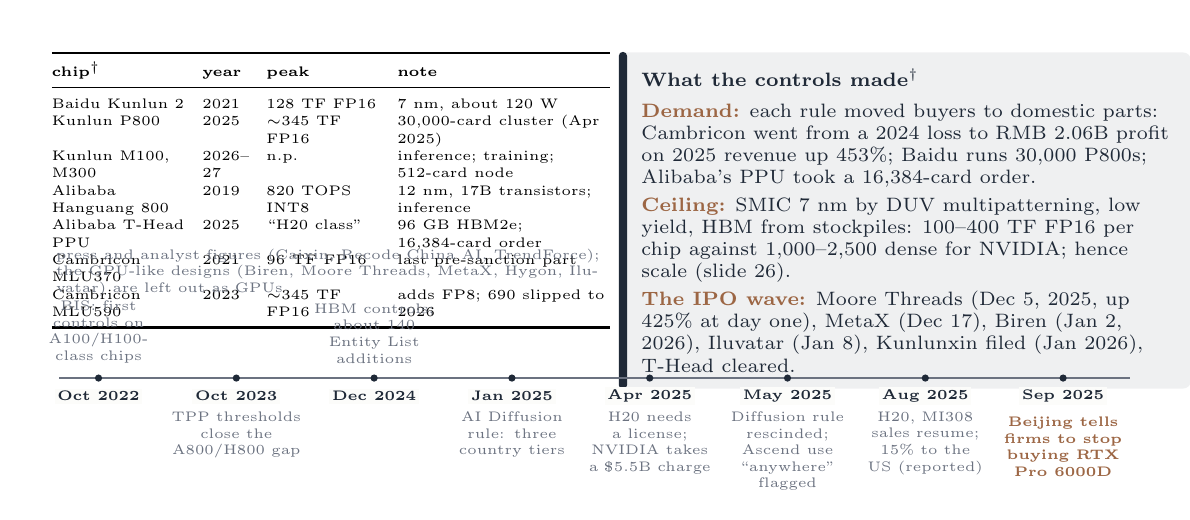
\begin{tikzpicture}
  \useasboundingbox (0,0) rectangle (14.4,5.9);
  \node[anchor=north west,inner sep=0,font=\fontsize{5.2}{6.2}\selectfont] at (0.3,5.6) {%
    \renewcommand{\arraystretch}{1.02}\setlength{\tabcolsep}{1.6pt}%
    \begin{tabular}{@{}>{\raggedright\arraybackslash}p{1.8cm}>{\raggedright\arraybackslash}p{0.7cm}>{\raggedright\arraybackslash}p{1.55cm}>{\raggedright\arraybackslash}p{2.7cm}@{}}
      \toprule
      \textbf{chip}$^\dagger$ & \textbf{year} & \textbf{peak} & \textbf{note}\\
      \midrule
      Baidu Kunlun 2 & 2021 & 128 TF FP16 & 7 nm, about 120 W\\
      Kunlun P800 & 2025 & ${\sim}$345 TF FP16 & 30{,}000-card cluster (Apr 2025)\\
      Kunlun M100, M300 & 2026--27 & n.p. & inference; training; 512-card node\\
      Alibaba Hanguang 800 & 2019 & 820 TOPS INT8 & 12 nm, 17B transistors; inference\\
      Alibaba T-Head PPU & 2025 & ``H20 class'' & 96 GB HBM2e; 16{,}384-card order\\
      Cambricon MLU370 & 2021 & 96 TF FP16 & last pre-sanction part\\
      Cambricon MLU590 & 2023 & ${\sim}$345 TF FP16 & adds FP8; 690 slipped to 2026\\
      \bottomrule
    \end{tabular}};
  \node[lab,font=\tiny,anchor=north west,text width=7.0cm] at (0.3,3.15) {press and analyst figures (Caixin, Recode China AI, TrendForce); the GPU-like designs (Biren, Moore Threads, MetaX, Hygon, Iluvatar) are left out as GPUs};
  \bgpanels{7.5}{5.6}{6.7cm}{What the controls made$^\dagger$}{%
    \hl{trn}{Demand:} each rule moved buyers to domestic parts:
    Cambricon went from a 2024 loss to RMB 2.06B profit on 2025
    revenue up 453\%; Baidu runs 30{,}000 P800s; Alibaba's PPU took
    a 16{,}384-card order.\\[2pt]
    \hl{trn}{Ceiling:} SMIC 7 nm by DUV multipatterning, low yield,
    HBM from stockpiles: 100--400 TF FP16 per chip against
    1{,}000--2{,}500 dense for NVIDIA; hence scale (slide 26).\\[2pt]
    \hl{trn}{The IPO wave:} Moore Threads (Dec 5, 2025, up 425\% at
    day one), MetaX (Dec 17), Biren (Jan 2, 2026), Iluvatar (Jan 8),
    Kunlunxin filed (Jan 2026), T-Head cleared.}
  % export-control timeline across the bottom
  \draw[muted,line width=0.8pt] (0.4,1.45) -- (14.0,1.45);
  \foreach \x in {0.9,2.65,4.4,6.15,7.9,9.65,11.4,13.15}{\fill[ink] (\x,1.45) circle (1.3pt);}
  \foreach \yr/\x in {Oct 2022/0.9,Oct 2023/2.65,Dec 2024/4.4,Jan 2025/6.15,Apr 2025/7.9,May 2025/9.65,Aug 2025/11.4,Sep 2025/13.15}{\node[font=\tiny\bfseries,text=ink,fill=paper,inner sep=1pt] at (\x,1.22) {\yr};}
  \node[lab,anchor=south,text width=1.7cm,align=center,font=\tiny] at (0.9,1.58) {BIS: first controls on A100/H100-class chips};
  \node[lab,anchor=north,text width=1.7cm,align=center,font=\tiny] at (2.65,1.08) {TPP thresholds close the A800/H800 gap};
  \node[lab,anchor=south,text width=1.7cm,align=center,font=\tiny] at (4.4,1.58) {HBM controls; about 140 Entity List additions};
  \node[lab,anchor=north,text width=1.7cm,align=center,font=\tiny] at (6.15,1.08) {AI Diffusion rule: three country tiers};
  \node[lab,anchor=north,text width=1.7cm,align=center,font=\tiny] at (7.9,1.08) {H20 needs a license; NVIDIA takes a \$5.5B charge};
  \node[lab,anchor=north,text width=1.7cm,align=center,font=\tiny] at (9.65,1.08) {Diffusion rule rescinded; Ascend use ``anywhere'' flagged};
  \node[lab,anchor=north,text width=1.7cm,align=center,font=\tiny] at (11.4,1.08) {H20, MI308 sales resume; 15\% to the US (reported)};
  \node[anchor=north,text width=1.7cm,align=center,font=\tiny\bfseries,text=trn] at (13.15,1.08) {Beijing tells firms to stop buying RTX Pro 6000D};
\end{tikzpicture}
\end{frame}

% ---------------------------------------------------------------- 28
\stage{8}
\begin{frame}{Compute in the memory: d-Matrix, Untether, Mythic, EnCharge}
\framesubtitle{Put the multiply in the SRAM array and the bytes stop moving; capacity and precision are the price.}
\centering
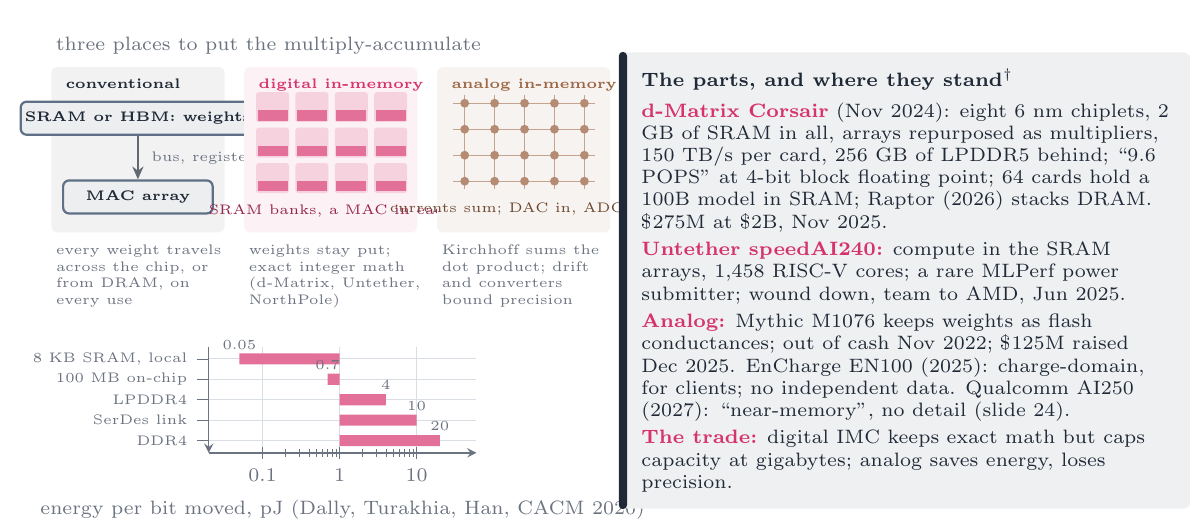
\begin{tikzpicture}
  \useasboundingbox (0,0) rectangle (14.4,5.9);
  \node[lab,anchor=south west] at (0.3,5.5) {three places to put the multiply-accumulate};
  % (a) conventional datapath
  \begin{scope}[shift={(0.3,3.3)}]
    \fill[ink!6,rounded corners=2pt] (0,0) rectangle (2.2,2.1);
    \node[font=\fontsize{5.2}{6}\selectfont\bfseries,text=ink,anchor=north west] at (0.06,2.07) {conventional};
    \node[comp=tok,minimum width=1.9cm,minimum height=0.42cm,font=\fontsize{4.6}{5.2}\selectfont\bfseries,text=ink,inner sep=1.5pt] (sram) at (1.1,1.45) {SRAM or HBM: weights};
    \node[comp=tok,minimum width=1.9cm,minimum height=0.42cm,font=\fontsize{4.6}{5.2}\selectfont\bfseries,text=ink,inner sep=1.5pt] (mac) at (1.1,0.45) {MAC array};
    \draw[flow] (sram) -- (mac);
    \node[font=\fontsize{4.2}{5}\selectfont,text=muted,anchor=west] at (1.15,0.95) {bus, registers};
  \end{scope}
  \node[lab,font=\tiny,anchor=north west,text width=2.2cm,align=flush left] at (0.3,3.2) {every weight travels across the chip, or from DRAM, on every use};
  % (b) digital in-memory compute
  \begin{scope}[shift={(2.75,3.3)}]
    \fill[outc!7,rounded corners=2pt] (0,0) rectangle (2.2,2.1);
    \node[font=\fontsize{5.2}{6}\selectfont\bfseries,text=outc,anchor=north west] at (0.06,2.07) {digital in-memory};
    \foreach \c in {0,1,2,3}{\foreach \r in {0,1,2}{
      \fill[outc!22,rounded corners=1pt] (0.15+\c*0.5,0.5+\r*0.45) rectangle ++(0.42,0.38);
      \fill[outc!70] (0.17+\c*0.5,0.52+\r*0.45) rectangle ++(0.38,0.13);}}
    \node[font=\fontsize{4.2}{5}\selectfont,text=outc!70!black,anchor=north] at (1.1,0.47) {SRAM banks, a MAC in each};
  \end{scope}
  \node[lab,font=\tiny,anchor=north west,text width=2.2cm,align=flush left] at (2.75,3.2) {weights stay put; exact integer math (d-Matrix, Untether, NorthPole)};
  % (c) analog compute-in-memory
  \begin{scope}[shift={(5.2,3.3)}]
    \fill[trn!8,rounded corners=2pt] (0,0) rectangle (2.2,2.1);
    \node[font=\fontsize{5.2}{6}\selectfont\bfseries,text=trn,anchor=north west] at (0.06,2.07) {analog in-memory};
    \foreach \c in {0,...,4}{\draw[trn!60,line width=0.5pt] (0.35+\c*0.38,0.55) -- (0.35+\c*0.38,1.75);}
    \foreach \r in {0,...,3}{\draw[trn!60,line width=0.5pt] (0.2,0.65+\r*0.33) -- (2.0,0.65+\r*0.33);}
    \foreach \c in {0,...,4}{\foreach \r in {0,...,3}{\fill[trn!75] (0.35+\c*0.38,0.65+\r*0.33) circle (1.6pt);}}
    \node[font=\fontsize{4.2}{5}\selectfont,text=trn!70!black,anchor=north] at (1.1,0.5) {currents sum; DAC in, ADC out};
  \end{scope}
  \node[lab,font=\tiny,anchor=north west,text width=2.2cm,align=flush left] at (5.2,3.2) {Kirchhoff sums the dot product; drift and converters bound precision};
  % energy per bit moved (Dally 2020)
  \begin{scope}[shift={(2.3,0.5)}]
  \begin{axis}[lecture,scale only axis,width=3.4cm,height=1.35cm,xbar,bar width=4pt,xmode=log,xmin=0.02,xmax=60,enlarge y limits=0.15,
      symbolic y coords={{8 KB SRAM, local},{100 MB on-chip},{LPDDR4},{SerDes link},{DDR4}},
      ytick=data,y dir=reverse,yticklabel style={font=\tiny},xlabel={energy per bit moved, pJ (Dally, Turakhia, Han, CACM 2020)},
      xtick={0.1,1,10},xticklabels={0.1,1,10},
      nodes near coords,nodes near coords style={font=\tiny,text=muted},point meta=explicit symbolic]
    \addplot[fill=outc!70,draw=none] coordinates {(0.05,{8 KB SRAM, local})[0.05] (0.7,{100 MB on-chip})[0.7] (4,{LPDDR4})[4] (10,{SerDes link})[10] (20,{DDR4})[20]};
  \end{axis}
  \end{scope}
  \bgpanels{7.5}{5.6}{6.7cm}{The parts, and where they stand$^\dagger$}{%
    \hl{outc}{d-Matrix Corsair} (Nov 2024): eight 6 nm chiplets, 2 GB of
    SRAM in all, arrays repurposed as multipliers, 150 TB/s per card,
    256 GB of LPDDR5 behind; ``9.6 POPS'' at 4-bit block floating
    point; 64 cards hold a 100B model in SRAM; Raptor (2026) stacks
    DRAM. \$275M at \$2B, Nov 2025.\\[2pt]
    \hl{outc}{Untether speedAI240:} compute in the SRAM arrays, 1{,}458
    RISC-V cores; a rare MLPerf power submitter; wound down, team to
    AMD, Jun 2025.\\[2pt]
    \hl{outc}{Analog:} Mythic M1076 keeps weights as flash
    conductances; out of cash Nov 2022; \$125M raised Dec
    2025. EnCharge EN100 (2025): charge-domain, for clients; no
    independent data. Qualcomm AI250 (2027): ``near-memory'', no
    detail (slide 24).\\[2pt]
    \hl{outc}{The trade:} digital IMC keeps exact math but caps
    capacity at gigabytes; analog saves energy, loses precision.}
\end{tikzpicture}
\end{frame}

% ---------------------------------------------------------------- 29
\begin{frame}{The specialization spectrum: from GPU to hardwired model}
\framesubtitle{Each step right trades freedom for speed; Taalas etched a model into metal and was bought in six months.}
\centering
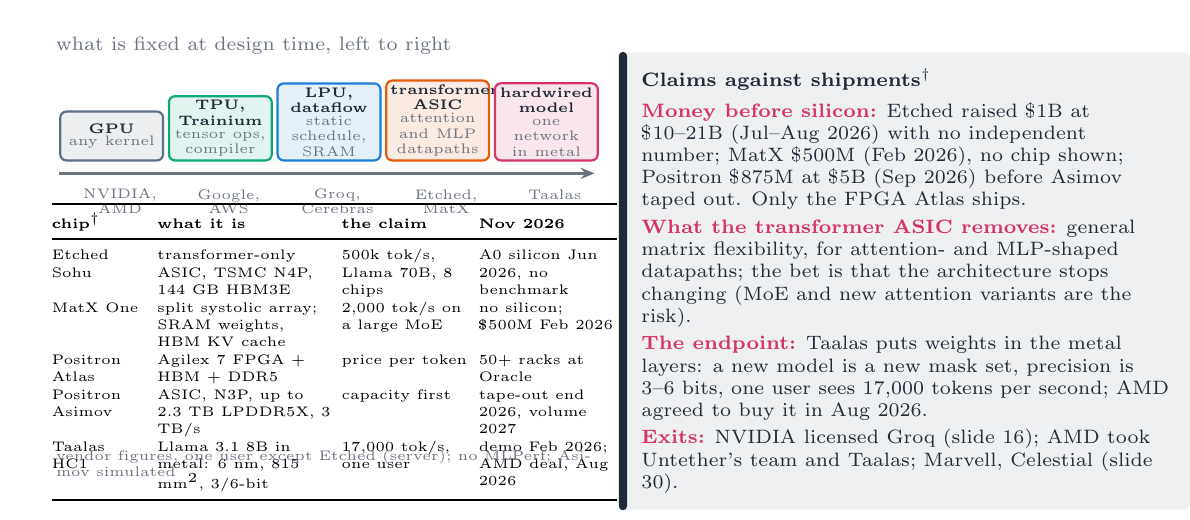
\begin{tikzpicture}
  \useasboundingbox (0,0) rectangle (14.4,5.9);
  \node[lab,anchor=south west] at (0.3,5.5) {what is fixed at design time, left to right};
  \draw[-{Stealth[length=5pt,width=4pt]},muted,line width=1.2pt] (0.4,4.05) -- (7.2,4.05);
  \foreach \x/\col/\lab/\sub in {0.4/tok/{GPU}/{any kernel},1.78/emb/{TPU, Trainium}/{tensor ops, compiler},3.16/mlp/{LPU, dataflow}/{static schedule, SRAM},4.54/attn/{transformer ASIC}/{attention and MLP datapaths},5.92/outc/{hardwired model}/{one network in metal}}{
    \node[comp=\col,minimum width=1.3cm,minimum height=0.62cm,font=\fontsize{4.8}{5.6}\selectfont\bfseries,text=ink,inner sep=1.5pt,anchor=south west,text width=1.2cm,align=center] at (\x,4.2) {\lab\\[-1pt]{\fontsize{4.2}{5}\selectfont\mdseries\color{muted}\sub}};}
  \foreach \x/\lab in {0.4/{NVIDIA, AMD},1.78/{Google, AWS},3.16/{Groq, Cerebras},4.54/{Etched, MatX},5.92/{Taalas}}{\node[font=\fontsize{4.6}{5.4}\selectfont,text=muted,anchor=north west,text width=1.3cm,align=center] at (\x,3.97) {\lab};}
  \node[anchor=north west,inner sep=0,font=\fontsize{5.2}{6.2}\selectfont] at (0.3,3.68) {%
    \renewcommand{\arraystretch}{1.04}\setlength{\tabcolsep}{2.0pt}%
    \begin{tabular}{@{}>{\raggedright\arraybackslash}p{1.2cm}>{\raggedright\arraybackslash}p{2.2cm}>{\raggedright\arraybackslash}p{1.6cm}>{\raggedright\arraybackslash}p{1.75cm}@{}}
      \toprule
      \textbf{chip}$^\dagger$ & \textbf{what it is} & \textbf{the claim} & \textbf{Nov 2026}\\
      \midrule
      Etched Sohu & transformer-only ASIC, TSMC N4P, 144 GB HBM3E & 500k tok/s, Llama 70B, 8 chips & A0 silicon Jun 2026, no benchmark\\
      MatX One & split systolic array; SRAM weights, HBM KV cache & 2{,}000 tok/s on a large MoE & no silicon; \$500M Feb 2026\\
      Positron Atlas & Agilex 7 FPGA $+$ HBM $+$ DDR5 & price per token & 50$+$ racks at Oracle\\
      Positron Asimov & ASIC, N3P, up to 2.3 TB LPDDR5X, 3 TB/s & capacity first & tape-out end 2026, volume 2027\\
      Taalas HC1 & Llama 3.1 8B in metal: 6 nm, 815 mm$^2$, 3/6-bit & 17{,}000 tok/s, one user & demo Feb 2026; AMD deal, Aug 2026\\
      \bottomrule
    \end{tabular}};
  \node[lab,font=\tiny,anchor=north west,text width=7.0cm] at (0.3,0.6) {vendor figures, one user except Etched (server); no MLPerf; Asimov simulated};
  \bgpanels{7.5}{5.6}{6.7cm}{Claims against shipments$^\dagger$}{%
    \hl{outc}{Money before silicon:} Etched raised \$1B at \$10--21B
    (Jul--Aug 2026) with no independent number; MatX
    \$500M (Feb 2026), no chip shown;
    Positron \$875M at \$5B (Sep 2026) before Asimov taped out. Only
    the FPGA Atlas ships.\\[2pt]
    \hl{outc}{What the transformer ASIC removes:} general matrix
    flexibility, for attention- and MLP-shaped datapaths; the bet is
    that the architecture stops changing (MoE and new attention
    variants are the risk).\\[2pt]
    \hl{outc}{The endpoint:} Taalas puts weights in the metal layers:
    a new model is a new mask set, precision is 3--6 bits, one user
    sees 17{,}000 tokens per second; AMD agreed to buy it in Aug 2026.\\[2pt]
    \hl{outc}{Exits:} NVIDIA licensed Groq (slide 16); AMD took
    Untether's team and Taalas; Marvell, Celestial (slide 30).}
\end{tikzpicture}
\end{frame}

% ---------------------------------------------------------------- 30
\begin{frame}{Light and spikes: photonics and neuromorphic computing}
\framesubtitle{Photonic compute was deferred and money went to interconnect; neuromorphic machines stay research tools.}
\centering
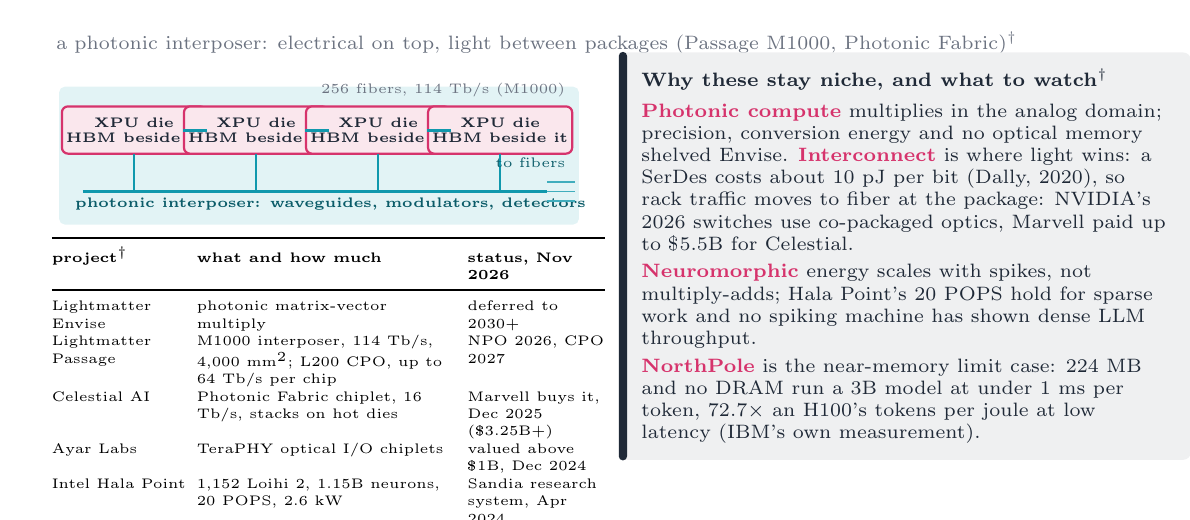
\begin{tikzpicture}
  \useasboundingbox (0,0) rectangle (14.4,5.9);
  \node[lab,anchor=south west] at (0.3,5.5) {a photonic interposer: electrical on top, light between packages (Passage M1000, Photonic Fabric)$^\dagger$};
  \begin{scope}[shift={(0.4,3.4)}]
    \fill[vc!12,rounded corners=2pt] (0,0) rectangle (6.6,1.75);
    \node[font=\fontsize{4.6}{5.4}\selectfont\bfseries,text=vc!60!black,anchor=south west] at (0.08,0.06) {photonic interposer: waveguides, modulators, detectors};
    \foreach \i in {0,1,2,3}{\node[comp=outc,minimum width=1.25cm,minimum height=0.6cm,font=\fontsize{4.6}{5.4}\selectfont\bfseries,text=ink,inner sep=1.5pt] (x\i) at (0.95+\i*1.55,1.2) {XPU die\\HBM beside it};}
    \draw[vc,line width=1.1pt] (x0.east) -- (x1.west); \draw[vc,line width=1.1pt] (x1.east) -- (x2.west); \draw[vc,line width=1.1pt] (x2.east) -- (x3.west);
    \foreach \i in {0,1,2,3}{\draw[vc,line width=0.9pt] (0.95+\i*1.55,0.9) -- (0.95+\i*1.55,0.42);}
    \draw[vc,line width=1.1pt] (0.3,0.42) -- (6.2,0.42);
    \foreach \y in {0.3,0.42,0.54}{\draw[vc!80,line width=0.6pt] (6.2,\y) -- (6.55,\y);}
    \node[font=\fontsize{4.4}{5}\selectfont,text=vc!60!black,anchor=south east] at (6.55,0.6) {to fibers};
    \node[font=\fontsize{4.4}{5}\selectfont,text=muted,anchor=south east] at (6.55,1.5) {256 fibers, 114 Tb/s (M1000)};
  \end{scope}
  \node[anchor=north west,inner sep=0,font=\fontsize{5.2}{6.2}\selectfont] at (0.3,3.25) {%
    \renewcommand{\arraystretch}{1.04}\setlength{\tabcolsep}{2.0pt}%
    \begin{tabular}{@{}>{\raggedright\arraybackslash}p{1.7cm}>{\raggedright\arraybackslash}p{3.3cm}>{\raggedright\arraybackslash}p{1.75cm}@{}}
      \toprule
      \textbf{project}$^\dagger$ & \textbf{what and how much} & \textbf{status, Nov 2026}\\
      \midrule
      Lightmatter Envise & photonic matrix-vector multiply & deferred to 2030$+$\\
      Lightmatter Passage & M1000 interposer, 114 Tb/s, 4{,}000 mm$^2$; L200 CPO, up to 64 Tb/s per chip & NPO 2026, CPO 2027\\
      Celestial AI & Photonic Fabric chiplet, 16 Tb/s, stacks on hot dies & Marvell buys it, Dec 2025 (\$3.25B$+$)\\
      Ayar Labs & TeraPHY optical I/O chiplets & valued above \$1B, Dec 2024\\
      Intel Hala Point & 1{,}152 Loihi 2, 1.15B neurons, 20 POPS, 2.6 kW & Sandia research system, Apr 2024\\
      IBM NorthPole & 12 nm, 22B transistors, 256 cores, 224 MB, no DRAM & prototype; 3B LLM on 16 cards\\
      \bottomrule
    \end{tabular}};
  \bgpanels{7.5}{5.6}{6.7cm}{Why these stay niche, and what to watch$^\dagger$}{%
    \hl{outc}{Photonic compute} multiplies in the analog domain;
    precision, conversion energy and no optical memory shelved Envise. \hl{outc}{Interconnect} is where light wins: a
    SerDes costs about 10 pJ per bit (Dally, 2020), so rack traffic
    moves to fiber at the package: NVIDIA's 2026 switches use
    co-packaged optics, Marvell paid up to \$5.5B for Celestial.\\[2pt]
    \hl{outc}{Neuromorphic} energy scales with spikes, not
    multiply-adds; Hala Point's 20 POPS hold for sparse work and no
    spiking machine has shown dense LLM throughput.\\[2pt]
    \hl{outc}{NorthPole} is the near-memory limit case: 224 MB and no
    DRAM run a 3B model at under 1 ms per token, 72.7$\times$ an H100's
    tokens per joule at low latency (IBM's own measurement).}
\end{tikzpicture}
\end{frame}

% ---------------------------------------------------------------- 31
\stage{9}
\begin{frame}{The chips side by side: what each vendor published}
\framesubtitle{Dense peaks, memory and fabric for eleven non-GPU parts against one GPU; the gaps (n.p.) are part of the picture.}
\centering
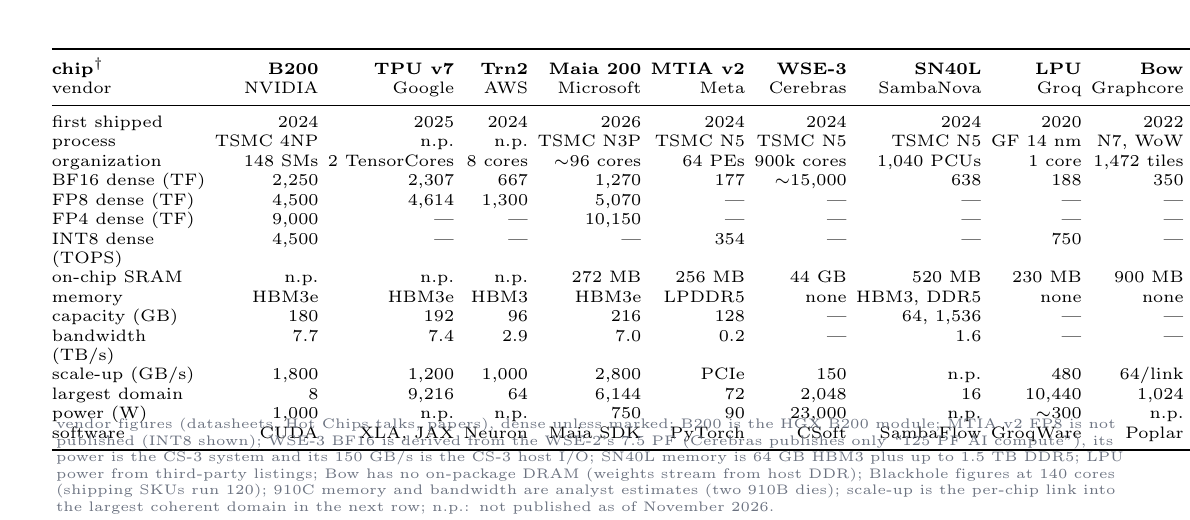
\begin{tikzpicture}
  \useasboundingbox (0,0) rectangle (14.4,5.9);
  \node[anchor=north west,inner sep=0,font=\fontsize{5.8}{6.9}\selectfont] at (0.3,5.65) {%
    \renewcommand{\arraystretch}{1.02}\setlength{\tabcolsep}{1.7pt}%
    \begin{tabular}{@{}>{\raggedright\arraybackslash}p{1.95cm}rrrrrrrrrrrr@{}}
      \toprule
      \textbf{chip}$^\dagger$ & \textbf{B200} & \textbf{TPU v7} & \textbf{Trn2} & \textbf{Maia 200} & \textbf{MTIA v2} & \textbf{WSE-3} & \textbf{SN40L} & \textbf{LPU} & \textbf{Bow} & \textbf{Blackhole} & \textbf{RNGD} & \textbf{910C}\\
      vendor & NVIDIA & Google & AWS & Microsoft & Meta & Cerebras & SambaNova & Groq & Graphcore & Tenstorrent & Furiosa & Huawei\\
      \midrule
      first shipped & 2024 & 2025 & 2024 & 2026 & 2024 & 2024 & 2024 & 2020 & 2022 & 2025 & 2026 & 2025\\
      process & TSMC 4NP & n.p. & n.p. & TSMC N3P & TSMC N5 & TSMC N5 & TSMC N5 & GF 14 nm & N7, WoW & TSMC N6 & TSMC N5 & SMIC N+2\\
      organization & 148 SMs & 2 TensorCores & 8 cores & ${\sim}$96 cores & 64 PEs & 900k cores & 1{,}040 PCUs & 1 core & 1{,}472 tiles & 140 Tensix & 8 PEs & 2 dies\\
      BF16 dense (TF) & 2{,}250 & 2{,}307 & 667 & 1{,}270 & 177 & ${\sim}$15{,}000 & 638 & 188 & 350 & 372 & 256 & ${\sim}$800\\
      FP8 dense (TF) & 4{,}500 & 4{,}614 & 1{,}300 & 5{,}070 & --- & --- & --- & --- & --- & 745 & 512 & ---\\
      FP4 dense (TF) & 9{,}000 & --- & --- & 10{,}150 & --- & --- & --- & --- & --- & --- & --- & ---\\
      INT8 dense (TOPS) & 4{,}500 & --- & --- & --- & 354 & --- & --- & 750 & --- & --- & --- & ---\\
      on-chip SRAM & n.p. & n.p. & n.p. & 272 MB & 256 MB & 44 GB & 520 MB & 230 MB & 900 MB & 210 MB & 256 MB & 192 MB\\
      memory & HBM3e & HBM3e & HBM3 & HBM3e & LPDDR5 & none & HBM3, DDR5 & none & none & GDDR6 & HBM3 & HBM2e\\
      capacity (GB) & 180 & 192 & 96 & 216 & 128 & --- & 64, 1{,}536 & --- & --- & 32 & 48 & 128\\
      bandwidth (TB/s) & 7.7 & 7.4 & 2.9 & 7.0 & 0.2 & --- & 1.6 & --- & --- & 0.5 & 1.5 & 3.2\\
      scale-up (GB/s) & 1{,}800 & 1{,}200 & 1{,}000 & 2{,}800 & PCIe & 150 & n.p. & 480 & 64/link & 400 & 128 & n.p.\\
      largest domain & 8 & 9{,}216 & 64 & 6{,}144 & 72 & 2{,}048 & 16 & 10{,}440 & 1{,}024 & 32 & 8 & 384\\
      power (W) & 1{,}000 & n.p. & n.p. & 750 & 90 & 23{,}000 & n.p. & ${\sim}$300 & n.p. & 300 & 180 & n.p.\\
      software & CUDA & XLA, JAX & Neuron & Maia SDK & PyTorch & CSoft & SambaFlow & GroqWare & Poplar & TT-Metal & Furiosa & CANN\\
      \bottomrule
    \end{tabular}};
  \node[lab,anchor=north west,text width=13.8cm,font=\tiny] at (0.3,1.0) {vendor figures (datasheets, Hot Chips talks, papers), dense unless marked; B200 is the HGX B200 module; MTIA v2 FP8 is not published (INT8 shown); WSE-3 BF16 is derived from the WSE-2's 7.5 PF (Cerebras publishes only ``125 PF AI compute''), its power is the CS-3 system and its 150 GB/s is the CS-3 host I/O; SN40L memory is 64 GB HBM3 plus up to 1.5 TB DDR5; LPU power from third-party listings; Bow has no on-package DRAM (weights stream from host DDR); Blackhole figures at 140 cores (shipping SKUs run 120); 910C memory and bandwidth are analyst estimates (two 910B dies); scale-up is the per-chip link into the largest coherent domain in the next row; n.p.: not published as of November 2026.};
\end{tikzpicture}
\end{frame}

% ---------------------------------------------------------------- 32
\begin{frame}{MLPerf: who shows up, and who never did}
\framesubtitle{The neutral chip benchmark: TPUs, Gaudi, the IPU and a few inference parts came; Cerebras and Groq never did.}
\centering
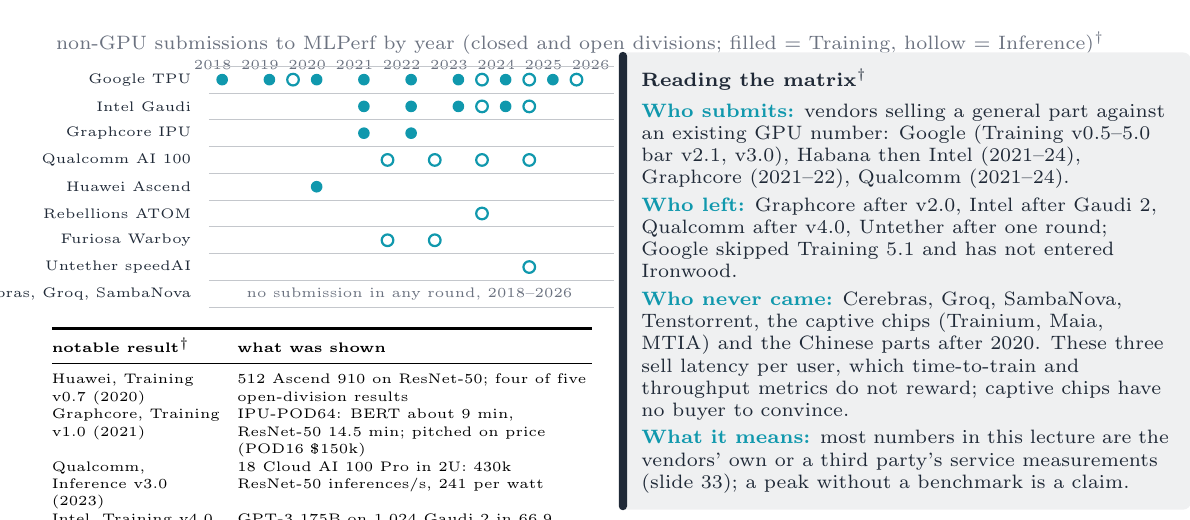
\begin{tikzpicture}
  \useasboundingbox (0,0) rectangle (14.4,5.9);
  % participation matrix: vendors x years
  \node[lab,anchor=south west] at (0.3,5.5) {non-GPU submissions to MLPerf by year (closed and open divisions; filled $=$ Training, hollow $=$ Inference)$^\dagger$};
  \begin{scope}[shift={(2.35,2.35)}]
    \foreach \y/\x in {2018/0,2019/0.6,2020/1.2,2021/1.8,2022/2.4,2023/3.0,2024/3.6,2025/4.2,2026/4.8}{\node[font=\tiny,text=muted,anchor=south] at (\x,2.9) {\y};}
    \foreach \lab/\r in {Google TPU/8,Intel Gaudi/7,Graphcore IPU/6,Qualcomm AI 100/5,Huawei Ascend/4,Rebellions ATOM/3,Furiosa Warboy/2,Untether speedAI/1,{Cerebras, Groq, SambaNova}/0}{
      \node[font=\tiny,text=ink,anchor=east] at (-0.15,\r*0.34+0.17) {\lab};
      \draw[muted!40,line width=0.3pt] (-0.05,\r*0.34) -- (5.1,\r*0.34);}
    \draw[muted!40,line width=0.3pt] (-0.05,9*0.34) -- (5.1,9*0.34);
    % Training (filled vc)
    \foreach \x in {0,0.6,1.2,1.8,2.4,3.0,3.6,4.2}{\fill[vc] (\x+0.12,8*0.34+0.17) circle (2.1pt);}
    \foreach \x in {1.8,2.4,3.0,3.6}{\fill[vc] (\x+0.12,7*0.34+0.17) circle (2.1pt);}
    \foreach \x in {1.8,2.4}{\fill[vc] (\x+0.12,6*0.34+0.17) circle (2.1pt);}
    \fill[vc] (1.2+0.12,4*0.34+0.17) circle (2.1pt);
    % Inference (hollow)
    \foreach \x in {0.6,3.0,3.6,4.2}{\draw[vc,line width=0.8pt] (\x+0.42,8*0.34+0.17) circle (2.1pt);}
    \foreach \x in {3.0,3.6}{\draw[vc,line width=0.8pt] (\x+0.42,7*0.34+0.17) circle (2.1pt);}
    \foreach \x in {1.8,2.4,3.0,3.6}{\draw[vc,line width=0.8pt] (\x+0.42,5*0.34+0.17) circle (2.1pt);}
    \draw[vc,line width=0.8pt] (3.0+0.42,3*0.34+0.17) circle (2.1pt);
    \foreach \x in {1.8,2.4}{\draw[vc,line width=0.8pt] (\x+0.42,2*0.34+0.17) circle (2.1pt);}
    \draw[vc,line width=0.8pt] (3.6+0.42,1*0.34+0.17) circle (2.1pt);
    \node[font=\tiny,text=muted] at (2.5,0.17) {no submission in any round, 2018--2026};
  \end{scope}
  \node[anchor=north west,inner sep=0,font=\fontsize{5.4}{6.3}\selectfont] at (0.3,2.1) {%
    \renewcommand{\arraystretch}{1.0}\setlength{\tabcolsep}{2.2pt}%
    \begin{tabular}{@{}>{\raggedright\arraybackslash}p{2.2cm}>{\raggedright\arraybackslash}p{4.5cm}@{}}
      \toprule
      \textbf{notable result}$^\dagger$ & \textbf{what was shown}\\
      \midrule
      Huawei, Training v0.7 (2020) & 512 Ascend 910 on ResNet-50; four of five open-division results\\
      Graphcore, Training v1.0 (2021) & IPU-POD64: BERT about 9 min, ResNet-50 14.5 min; pitched on price (POD16 \$150k)\\
      Qualcomm, Inference v3.0 (2023) & 18 Cloud AI 100 Pro in 2U: 430k ResNet-50 inferences/s, 241 per watt\\
      Intel, Training v4.0 (2024) & GPT-3 175B on 1{,}024 Gaudi 2 in 66.9 min; Gaudi 3 never appeared\\
      Google, Training v4.1 (2024) & Trillium preview and v5p pods on GPT-3 175B, 99\% weak scaling (Google's figure)\\
      \bottomrule
    \end{tabular}};
  \bgpanels{7.5}{5.6}{6.7cm}{Reading the matrix$^\dagger$}{%
    \hl{vc}{Who submits:} vendors selling a general part against an
    existing GPU number: Google (Training v0.5--5.0 bar v2.1,
    v3.0), Habana then Intel (2021--24), Graphcore (2021--22),
    Qualcomm (2021--24).\\[2pt]
    \hl{vc}{Who left:} Graphcore after v2.0, Intel after Gaudi 2,
    Qualcomm after v4.0, Untether after one round; Google skipped
    Training 5.1 and has not entered Ironwood.\\[2pt]
    \hl{vc}{Who never came:} Cerebras, Groq, SambaNova, Tenstorrent,
    the captive chips (Trainium, Maia, MTIA) and the Chinese parts
    after 2020. These three sell latency per user, which
    time-to-train and throughput metrics do not reward; captive
    chips have no buyer to convince.\\[2pt]
    \hl{vc}{What it means:} most numbers in this lecture are the
    vendors' own or a third party's service measurements (slide
    33); a peak without a benchmark is a claim.}
\end{tikzpicture}
\end{frame}

% ---------------------------------------------------------------- 33
\begin{frame}{Inference speed and price: what the SRAM machines deliver}
\framesubtitle{Thousands of tokens per second for one user, third-party measured; the catch is the cost per token.}
\centering
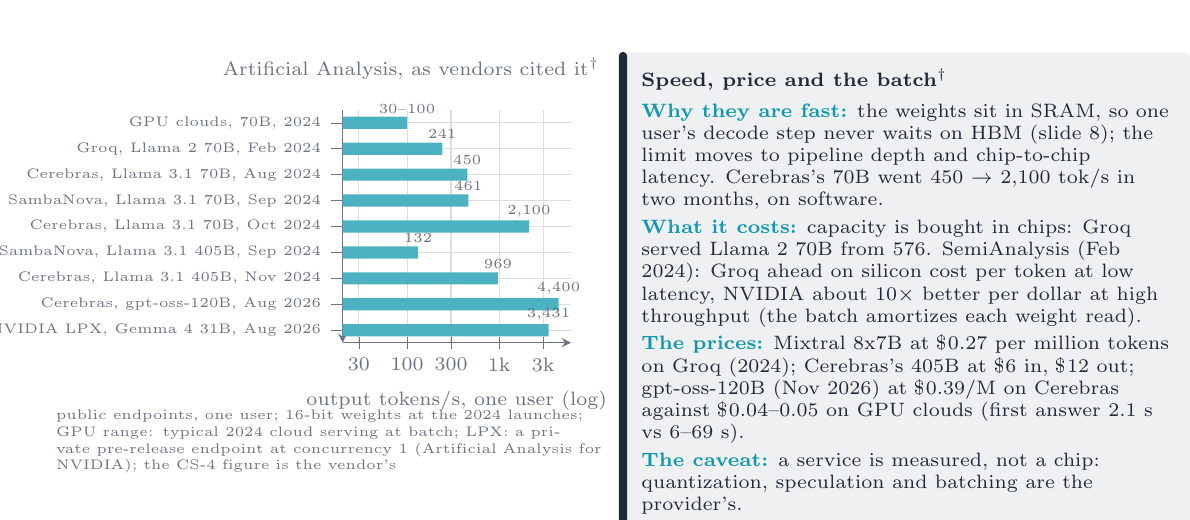
\begin{tikzpicture}
  \useasboundingbox (0,0) rectangle (14.4,5.9);
  \begin{scope}[shift={(4.0,1.9)}]
  \begin{axis}[lecture,scale only axis,width=2.9cm,height=2.95cm,xbar,bar width=4.4pt,xmode=log,log origin=infty,xmin=20,xmax=6000,enlarge y limits=0.06,
      symbolic y coords={{GPU clouds, 70B, 2024},{Groq, Llama 2 70B, Feb 2024},{Cerebras, Llama 3.1 70B, Aug 2024},{SambaNova, Llama 3.1 70B, Sep 2024},{Cerebras, Llama 3.1 70B, Oct 2024},{SambaNova, Llama 3.1 405B, Sep 2024},{Cerebras, Llama 3.1 405B, Nov 2024},{Cerebras, gpt-oss-120B, Aug 2026},{NVIDIA LPX, Gemma 4 31B, Aug 2026}},
      ytick=data,y dir=reverse,yticklabel style={font=\fontsize{4.6}{5}\selectfont},xlabel={output tokens/s, one user (log)},
      xtick={30,100,300,1000,3000},xticklabels={30,100,300,1k,3k},
      nodes near coords,nodes near coords style={font=\tiny,text=muted},point meta=explicit symbolic,
      title style={font=\scriptsize,text=muted,at={(0.3,1.02)}},title={Artificial Analysis, as vendors cited it$^\dagger$}]
    \addplot[fill=vc!75,draw=none] coordinates {(100,{GPU clouds, 70B, 2024})[30--100] (241,{Groq, Llama 2 70B, Feb 2024})[241] (450,{Cerebras, Llama 3.1 70B, Aug 2024})[450] (461,{SambaNova, Llama 3.1 70B, Sep 2024})[461] (2100,{Cerebras, Llama 3.1 70B, Oct 2024})[2{,}100] (132,{SambaNova, Llama 3.1 405B, Sep 2024})[132] (969,{Cerebras, Llama 3.1 405B, Nov 2024})[969] (4400,{Cerebras, gpt-oss-120B, Aug 2026})[4{,}400] (3431,{NVIDIA LPX, Gemma 4 31B, Aug 2026})[3{,}431]};
  \end{axis}
  \end{scope}
  \node[lab,font=\tiny,anchor=north west,text width=7.2cm] at (0.3,1.1) {public endpoints, one user; 16-bit weights at the 2024 launches; GPU range: typical 2024 cloud serving at batch; LPX: a private pre-release endpoint at concurrency 1 (Artificial Analysis for NVIDIA); the CS-4 figure is the vendor's};
  \bgpanels{7.5}{5.6}{6.7cm}{Speed, price and the batch$^\dagger$}{%
    \hl{vc}{Why they are fast:} the weights sit in SRAM, so one
    user's decode step never waits on HBM (slide 8); the limit moves
    to pipeline depth and chip-to-chip latency. Cerebras's 70B went
    450 $\to$ 2{,}100 tok/s in two months, on software.\\[2pt]
    \hl{vc}{What it costs:} capacity is bought in chips: Groq served
    Llama 2 70B from 576. SemiAnalysis (Feb 2024): Groq ahead on
    silicon cost per token at low latency, NVIDIA about 10$\times$
    better per dollar at high throughput (the batch amortizes each
    weight read).\\[2pt]
    \hl{vc}{The prices:} Mixtral 8x7B at \$0.27 per million tokens
    on Groq (2024); Cerebras's 405B at \$6 in, \$12 out;
    gpt-oss-120B (Nov 2026) at \$0.39/M on Cerebras against
    \$0.04--0.05 on GPU clouds (first answer 2.1 s vs 6--69 s).\\[2pt]
    \hl{vc}{The caveat:} a service is measured, not a chip:
    quantization, speculation and batching are the provider's.}
\end{tikzpicture}
\end{frame}

% ---------------------------------------------------------------- 34
\begin{frame}{Deals and share, 2025--26: commitments are not deployments}
\framesubtitle{The non-GPU chips won gigawatt-scale orders for the first time; most of that power is not yet installed.}
\centering
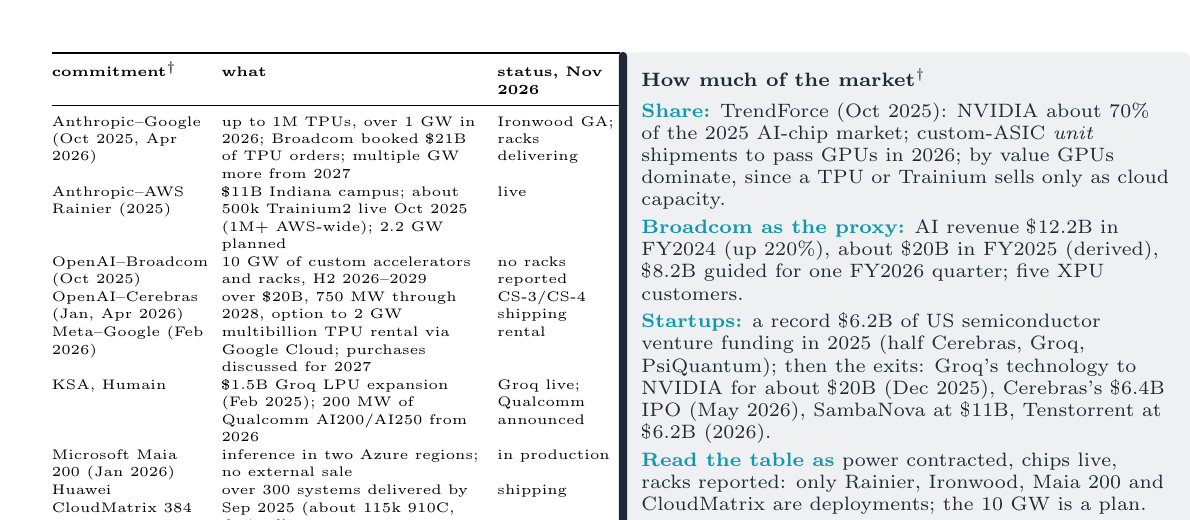
\begin{tikzpicture}
  \useasboundingbox (0,0) rectangle (14.4,5.9);
  \node[anchor=north west,inner sep=0,font=\fontsize{5.4}{6.3}\selectfont] at (0.3,5.6) {%
    \renewcommand{\arraystretch}{1.02}\setlength{\tabcolsep}{2.2pt}%
    \begin{tabular}{@{}>{\raggedright\arraybackslash}p{2.0cm}>{\raggedright\arraybackslash}p{3.35cm}>{\raggedright\arraybackslash}p{1.55cm}@{}}
      \toprule
      \textbf{commitment}$^\dagger$ & \textbf{what} & \textbf{status, Nov 2026}\\
      \midrule
      Anthropic--Google (Oct 2025, Apr 2026) & up to 1M TPUs, over 1 GW in 2026; Broadcom booked \$21B of TPU orders; multiple GW more from 2027 & Ironwood GA; racks delivering\\
      Anthropic--AWS Rainier (2025) & \$11B Indiana campus; about 500k Trainium2 live Oct 2025 (1M$+$ AWS-wide); 2.2 GW planned & live\\
      OpenAI--Broadcom (Oct 2025) & 10 GW of custom accelerators and racks, H2 2026--2029 & no racks reported\\
      OpenAI--Cerebras (Jan, Apr 2026) & over \$20B, 750 MW through 2028, option to 2 GW & CS-3/CS-4 shipping\\
      Meta--Google (Feb 2026) & multibillion TPU rental via Google Cloud; purchases discussed for 2027 & rental\\
      KSA, Humain & \$1.5B Groq LPU expansion (Feb 2025); 200 MW of Qualcomm AI200/AI250 from 2026 & Groq live; Qualcomm announced\\
      Microsoft Maia 200 (Jan 2026) & inference in two Azure regions; no external sale & in production\\
      Huawei CloudMatrix 384 & over 300 systems delivered by Sep 2025 (about 115k 910C, derived) & shipping\\
      \bottomrule
    \end{tabular}};
  \bgpanels{7.5}{5.6}{6.7cm}{How much of the market$^\dagger$}{%
    \hl{vc}{Share:} TrendForce (Oct 2025): NVIDIA about 70\% of the
    2025 AI-chip market; custom-ASIC \emph{unit} shipments to pass
    GPUs in 2026; by value GPUs dominate, since a TPU or Trainium
    sells only as cloud capacity.\\[2pt]
    \hl{vc}{Broadcom as the proxy:} AI revenue \$12.2B in FY2024 (up
    220\%), about \$20B in FY2025 (derived), \$8.2B guided for one
    FY2026 quarter; five XPU customers.\\[2pt]
    \hl{vc}{Startups:} a record \$6.2B of US semiconductor venture
    funding in 2025 (half Cerebras, Groq, PsiQuantum); then the
    exits: Groq's technology to NVIDIA for about \$20B (Dec 2025),
    Cerebras's \$6.4B IPO (May 2026), SambaNova at \$11B,
    Tenstorrent at \$6.2B (2026).\\[2pt]
    \hl{vc}{Read the table as} power contracted, chips live, racks
    reported: only Rainier, Ironwood, Maia 200 and CloudMatrix are
    deployments; the 10 GW is a plan.}
\end{tikzpicture}
\end{frame}

% ---------------------------------------------------------------- 35
\stage{10}
\begin{frame}{Why most of them failed, and what the survivors share}
\framesubtitle{A few found captive volume, a niche or a buyer for their IP; the rest ran out of software or money.}
\centering
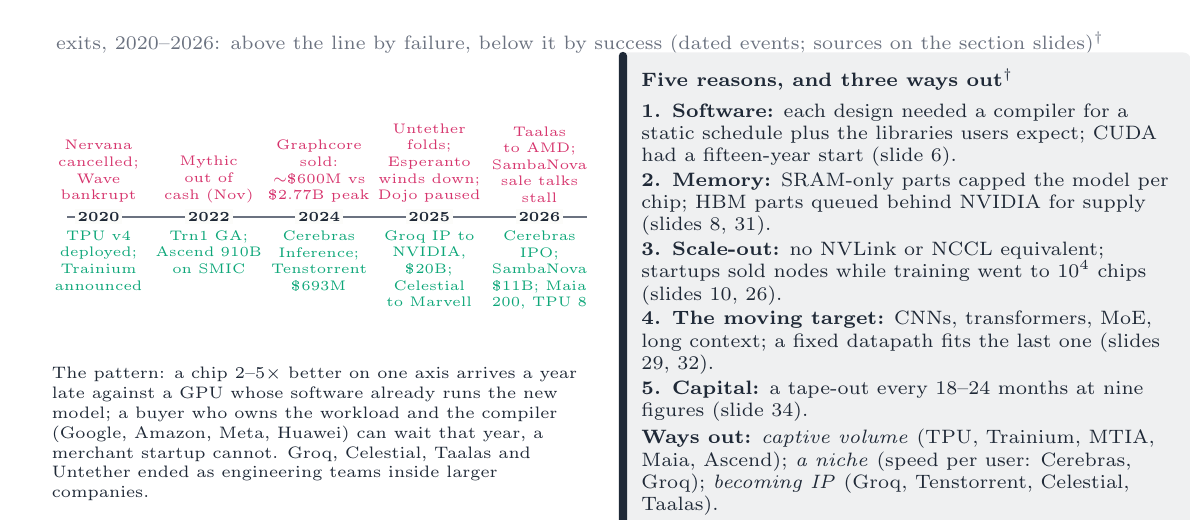
\begin{tikzpicture}
  \useasboundingbox (0,0) rectangle (14.4,5.9);
  \node[lab,anchor=south west] at (0.3,5.5) {exits, 2020--2026: above the line by failure, below it by success (dated events; sources on the section slides)$^\dagger$};
  \draw[muted,line width=0.8pt] (0.5,3.5) -- (7.1,3.5);
  \foreach \yr/\x in {2020/0.9,2022/2.3,2024/3.7,2025/5.1,2026/6.5}{\fill[ink] (\x,3.5) circle (1.3pt);\node[font=\tiny\bfseries,text=ink,fill=paper,inner sep=1pt] at (\x,3.5) {\yr};}
  \node[lab,anchor=south,text width=1.35cm,align=center,font=\tiny,text=outc] at (0.9,3.62) {Nervana cancelled; Wave bankrupt};
  \node[lab,anchor=south,text width=1.35cm,align=center,font=\tiny,text=outc] at (2.3,3.62) {Mythic out of cash (Nov)};
  \node[lab,anchor=south,text width=1.35cm,align=center,font=\tiny,text=outc] at (3.7,3.62) {Graphcore sold: ${\sim}$\$600M vs \$2.77B peak};
  \node[lab,anchor=south,text width=1.35cm,align=center,font=\tiny,text=outc] at (5.1,3.62) {Untether folds; Esperanto winds down; Dojo paused};
  \node[lab,anchor=south,text width=1.35cm,align=center,font=\tiny,text=outc] at (6.5,3.62) {Taalas to AMD; SambaNova sale talks stall};
  \node[lab,anchor=north,text width=1.35cm,align=center,font=\tiny,text=emb] at (0.9,3.38) {TPU v4 deployed; Trainium announced};
  \node[lab,anchor=north,text width=1.35cm,align=center,font=\tiny,text=emb] at (2.3,3.38) {Trn1 GA; Ascend 910B on SMIC};
  \node[lab,anchor=north,text width=1.35cm,align=center,font=\tiny,text=emb] at (3.7,3.38) {Cerebras Inference; Tenstorrent \$693M};
  \node[lab,anchor=north,text width=1.35cm,align=center,font=\tiny,text=emb] at (5.1,3.38) {Groq IP to NVIDIA, \$20B; Celestial to Marvell};
  \node[lab,anchor=north,text width=1.35cm,align=center,font=\tiny,text=emb] at (6.5,3.38) {Cerebras IPO; SambaNova \$11B; Maia 200, TPU 8};
  \node[anchor=north west,inner sep=0,font=\fontsize{6}{7.2}\selectfont,text=ink,text width=6.9cm,align=flush left] at (0.3,1.6) {%
    The pattern: a chip 2--5$\times$ better on one axis arrives a year
    late against a GPU whose software already runs the new model; a
    buyer who owns the workload and the compiler (Google, Amazon,
    Meta, Huawei) can wait that year, a merchant startup cannot.
    Groq, Celestial, Taalas and Untether ended as engineering teams
    inside larger companies.};
  \bgpanels{7.5}{5.6}{6.7cm}{Five reasons, and three ways out$^\dagger$}{%
    \hl{ink}{1. Software:} each design needed a compiler for a static
    schedule plus the libraries users expect; CUDA had a
    fifteen-year start (slide 6).\\[1pt]
    \hl{ink}{2. Memory:} SRAM-only parts capped the model per chip;
    HBM parts queued behind NVIDIA for supply (slides 8, 31).\\[1pt]
    \hl{ink}{3. Scale-out:} no NVLink or NCCL equivalent; startups
    sold nodes while training went to 10$^4$ chips (slides 10, 26).\\[1pt]
    \hl{ink}{4. The moving target:} CNNs, transformers, MoE, long
    context; a fixed datapath fits the last one (slides 29, 32).\\[1pt]
    \hl{ink}{5. Capital:} a tape-out every 18--24 months at nine
    figures (slide 34).\\[2pt]
    \hl{ink}{Ways out:} \emph{captive volume} (TPU, Trainium, MTIA,
    Maia, Ascend); \emph{a niche} (speed per user: Cerebras, Groq);
    \emph{becoming IP} (Groq, Tenstorrent, Celestial, Taalas).}
\end{tikzpicture}
\end{frame}

% ---------------------------------------------------------------- 36
\begin{frame}{Summary: what to take from this lecture}
\framesubtitle{The rivals won where someone else owned the workload; the 2027 questions are about scale, not cores.}
\centering
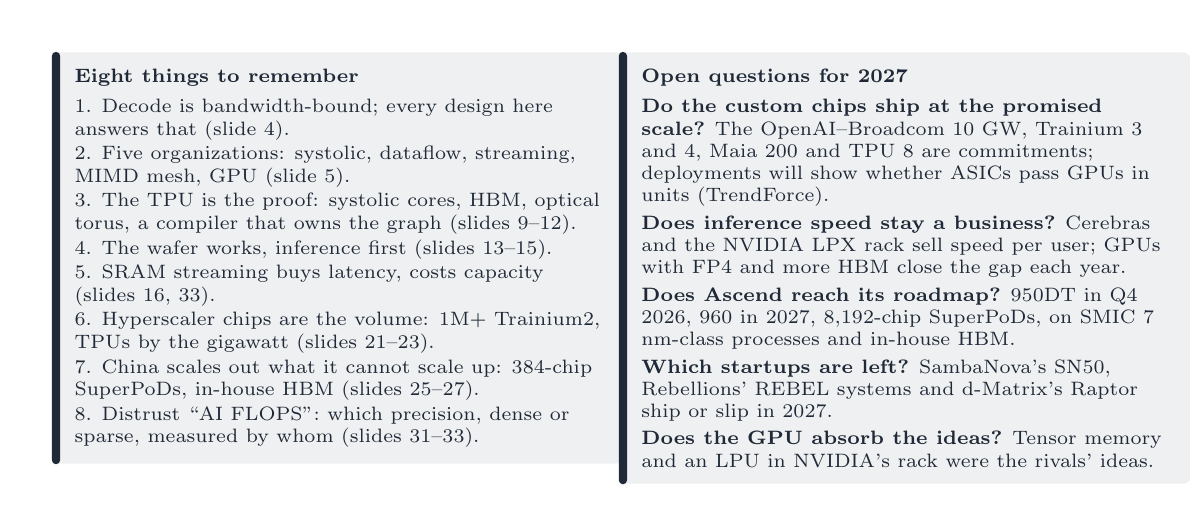
\begin{tikzpicture}
  \useasboundingbox (0,0) rectangle (14.4,5.9);
  \bgpanels{0.3}{5.6}{6.7cm}{Eight things to remember}{%
    1. Decode is bandwidth-bound; every design here answers that
    (slide 4).\\[1pt]
    2. Five organizations: systolic, dataflow, streaming, MIMD mesh,
    GPU (slide 5).\\[1pt]
    3. The TPU is the proof: systolic cores, HBM, optical torus, a
    compiler that owns the graph (slides 9--12).\\[1pt]
    4. The wafer works, inference first (slides 13--15).\\[1pt]
    5. SRAM streaming buys latency, costs capacity (slides 16, 33).\\[1pt]
    6. Hyperscaler chips are the volume: 1M$+$ Trainium2, TPUs
    by the gigawatt (slides 21--23).\\[1pt]
    7. China scales out what it cannot scale up: 384-chip SuperPoDs,
    in-house HBM (slides 25--27).\\[1pt]
    8. Distrust ``AI FLOPS'': which precision, dense or sparse,
    measured by whom (slides 31--33).}
  \bgpanels{7.5}{5.6}{6.7cm}{Open questions for 2027}{%
    \hl{ink}{Do the custom chips ship at the promised scale?} The
    OpenAI--Broadcom 10 GW, Trainium 3 and 4, Maia 200 and TPU 8 are
    commitments; deployments will show whether ASICs pass GPUs in
    units (TrendForce).\\[2pt]
    \hl{ink}{Does inference speed stay a business?} Cerebras and the
    NVIDIA LPX rack sell speed per user; GPUs with FP4 and more HBM
    close the gap each year.\\[2pt]
    \hl{ink}{Does Ascend reach its roadmap?} 950DT in Q4 2026, 960 in
    2027, 8{,}192-chip SuperPoDs, on SMIC 7 nm-class processes and
    in-house HBM.\\[2pt]
    \hl{ink}{Which startups are left?} SambaNova's SN50, Rebellions'
    REBEL systems and d-Matrix's Raptor ship or slip in 2027.\\[2pt]
    \hl{ink}{Does the GPU absorb the ideas?} Tensor memory and an LPU
    in NVIDIA's rack were the rivals' ideas.}
\end{tikzpicture}
\end{frame}

% ---------------------------------------------------------------- 37
\begin{frame}{Sources}
\framesubtitle{Papers and talks, vendor documentation, filings, benchmark tables and reporting; $^\dagger$ marks vendor or press material.}
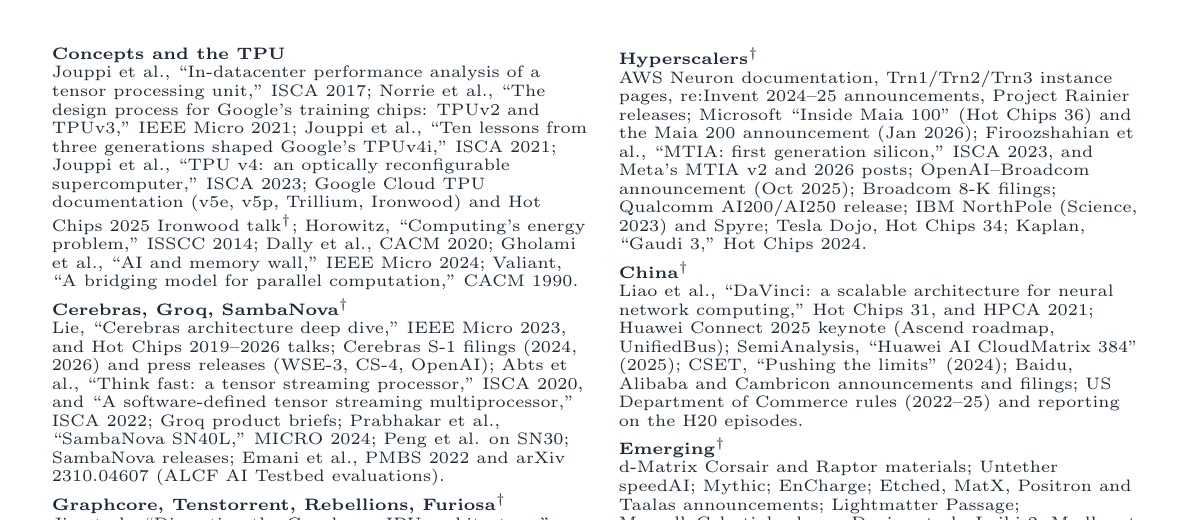
\begin{tikzpicture}
  \useasboundingbox (0,0) rectangle (14.4,5.9);
  \node[anchor=north west,inner sep=0,text width=6.8cm,font=\fontsize{5.6}{6.7}\selectfont,text=ink,align=flush left] at (0.3,5.65) {%
    \textbf{Concepts and the TPU}\\
    Jouppi et al., ``In-datacenter performance analysis of a tensor processing unit,'' ISCA 2017; Norrie et al., ``The design process for Google's training chips: TPUv2 and TPUv3,'' IEEE Micro 2021; Jouppi et al., ``Ten lessons from three generations shaped Google's TPUv4i,'' ISCA 2021; Jouppi et al., ``TPU v4: an optically reconfigurable supercomputer,'' ISCA 2023; Google Cloud TPU documentation (v5e, v5p, Trillium, Ironwood) and Hot Chips 2025 Ironwood talk$^\dagger$; Horowitz, ``Computing's energy problem,'' ISSCC 2014; Dally et al., CACM 2020; Gholami et al., ``AI and memory wall,'' IEEE Micro 2024; Valiant, ``A bridging model for parallel computation,'' CACM 1990.\\[2pt]
    \textbf{Cerebras, Groq, SambaNova}$^\dagger$\\
    Lie, ``Cerebras architecture deep dive,'' IEEE Micro 2023, and Hot Chips 2019--2026 talks; Cerebras S-1 filings (2024, 2026) and press releases (WSE-3, CS-4, OpenAI); Abts et al., ``Think fast: a tensor streaming processor,'' ISCA 2020, and ``A software-defined tensor streaming multiprocessor,'' ISCA 2022; Groq product briefs; Prabhakar et al., ``SambaNova SN40L,'' MICRO 2024; Peng et al. on SN30; SambaNova releases; Emani et al., PMBS 2022 and arXiv 2310.04607 (ALCF AI Testbed evaluations).\\[2pt]
    \textbf{Graphcore, Tenstorrent, Rebellions, Furiosa}$^\dagger$\\
    Jia et al., ``Dissecting the Graphcore IPU architecture,'' arXiv 1912.03413; Knowles, Hot Chips 33; Graphcore and SoftBank announcements; Vasiljevic and Capalija, ``Blackhole and TT-Metalium,'' Hot Chips 36; Tenstorrent datasheets and funding releases; Rebellions ISSCC 2024 and 2026 papers, Hot Chips 2025; FuriosaAI RNGD, ISCA 2024 industry track and Hot Chips 36; MLCommons result tables.};
  \node[anchor=north west,inner sep=0,text width=6.6cm,font=\fontsize{5.6}{6.7}\selectfont,text=ink,align=flush left] at (7.5,5.65) {%
    \textbf{Hyperscalers}$^\dagger$\\
    AWS Neuron documentation, Trn1/Trn2/Trn3 instance pages, re:Invent 2024--25 announcements, Project Rainier releases; Microsoft ``Inside Maia 100'' (Hot Chips 36) and the Maia 200 announcement (Jan 2026); Firoozshahian et al., ``MTIA: first generation silicon,'' ISCA 2023, and Meta's MTIA v2 and 2026 posts; OpenAI--Broadcom announcement (Oct 2025); Broadcom 8-K filings; Qualcomm AI200/AI250 release; IBM NorthPole (Science, 2023) and Spyre; Tesla Dojo, Hot Chips 34; Kaplan, ``Gaudi 3,'' Hot Chips 2024.\\[2pt]
    \textbf{China}$^\dagger$\\
    Liao et al., ``DaVinci: a scalable architecture for neural network computing,'' Hot Chips 31, and HPCA 2021; Huawei Connect 2025 keynote (Ascend roadmap, UnifiedBus); SemiAnalysis, ``Huawei AI CloudMatrix 384'' (2025); CSET, ``Pushing the limits'' (2024); Baidu, Alibaba and Cambricon announcements and filings; US Department of Commerce rules (2022--25) and reporting on the H20 episodes.\\[2pt]
    \textbf{Emerging}$^\dagger$\\
    d-Matrix Corsair and Raptor materials; Untether speedAI; Mythic; EnCharge; Etched, MatX, Positron and Taalas announcements; Lightmatter Passage; Marvell--Celestial release; Davies et al., Loihi 2; Modha et al., NorthPole, Science 2023.\\[2pt]
    \textbf{Measured and money}\\
    MLCommons Training v0.5--6.0 and Inference v0.5--6.0 result tables; Artificial Analysis provider benchmarks; SemiAnalysis, ``Groq inference tokenomics'' (2024); TrendForce (Oct 2025); Crunchbase News (Jan 2026); company filings and press releases for the deals table. Full list with links in the paper kit.};
\end{tikzpicture}
\end{frame}
\end{document}
